\documentclass[11pt, oneside]{article}   	% use "amsart" instead of "article" for AMSLaTeX format
\usepackage{geometry}                		% See geometry.pdf to learn the layout options. There are lots.
\geometry{letterpaper}                   		% ... or a4paper or a5paper or ... 
%\geometry{landscape}                		% Activate for rotated page geometry
%\usepackage[parfill]{parskip}    		% Activate to begin paragraphs with an empty line rather than an indent
%\usepackage{biblatex}
%\usepackage[comma,square,numbers,sort&compress]{natbib}
\usepackage{multirow}
\usepackage{multicolumn}
\usepackage{amsmath}

\usepackage{color}
\usepackage{rotating}
\usepackage{graphicx}				% Use pdf, png, jpg, or eps§ with pdflatex; use eps in DVI mode
								% TeX will automatically convert eps --> pdf in pdflatex		
\usepackage{amssymb}
\usepackage{hyperref}
\usepackage{bm}
\usepackage{lineno}
\usepackage[nottoc]{tocbibind}


\newcommand{\xis}{$\Xi(1530)^{0}$ }
\newcommand{\xisb}{$\overline{\Xi(1530)^{0}}$ }

\newcommand{\xiss}{$\Xi^{*0}$ }

\newcommand{\pt}{$\ensuremath{p_{\mathrm{T}}}$}
\newcommand{\mpt}{\langle p_{\mathrm{T}}\rangle}
\newcommand{\dedx}{d$E$/d$x$}
\newcommand{\dndy}{d$N$/d$y$}

\newcommand{\pbar}{$\rm\overline{p}$}
\newcommand{\Bbar}{$\rm\overline{B}$}
\newcommand{\Lbar}{$\rm\overline{\Lambda}$}
\newcommand{\La}{$\Lambda$}
\newcommand{\p}{\mbox{p}}
\newcommand{\pip}{$\pi^{+}$}
\newcommand{\pim}{$\pi^{-}$}
\newcommand{\kap}{$K^{+}$}
\newcommand{\kam}{$K^{-}$}
\newcommand{\degree}{$^{\rm o}$}
\newcommand{\s}{$\sqrt{s}$}
\newcommand{\snn}{$\sqrt{s_{\rm NN}}$}
\newcommand{\be}{\begin{equation}}
\newcommand{\ee}{\end{equation}}
\newcommand{\cL}{\textit{c}}
\newcommand{\AGeV}[1][ ]{$A$~GeV{#1}}
\newcommand{\mmass} {\mbox{\rm MeV$\kern-0.15em /\kern-0.12em c^2$} }
\newcommand {\Gmass} {\mbox{\rm GeV$\kern-0.15em /\kern-0.12em c^2$} }
\newcommand {\gmom}   {\mbox{\rm GeV$\kern-0.15em /\kern-0.12em c$} }
\newcommand {\mmom}   {\mbox{\rm MeV$\kern-0.15em /\kern-0.12em c$} }

\newcommand{\meandNdeta}{\ensuremath{\langle$d$N_{\mathrm{ch}}$/d$\eta_{\mathrm{lab}}\rangle}}
\newcommand{\dndydpt}{${\rm d}^2N/({\rm d}p_{\rm T}{\rm d}y)$}



\def\muB{$\mu_B$}
\def\muS{$\mu_S$}




%SetFonts

%SetFonts


\title{Study of the multi-strange resonance \xis production with ALICE at the LHC energies}
\author{Jihye Song}
\date{}							% Activate to display a given date or no date

\linenumbers

\begin{document}

\maketitle
\newpage

\tableofcontents
\newpage

\listoffigures
\newpage

\listoftables
\newpage


\section{The physics of relativistic heavy-ion collisions}

The main objective of relativistic heavy ion physics is to study the nuclear matter under extreme conditions which are high temperature and energy density. In these conditions, the Standard Model anticipates that the nuclear matter undergo a new phase, where the quarks and the gluons are expected to be de-confined called quark-gluon plasma (QGP) and to freely move. %The Standard Model is the theory of the elementary particles and their fundamental interactions. This theory includes the strong interactions due to the color charges of quarks and gluons and a combined theory of weak and electromagnetic interactions.



 %study QCD in a regime of of high temperature, high density, and large reaction volumes. The relativistic heavy ions physics is aimed at the application of this theory to complex and evolving systems of finite size, in order to understand the relations between collective phenomena and the microscopic laws of elementary-particle physics. The collisions between relativistic heavy ions allow to study the nuclear matter under conditions of extremely high temperature and energy density. In these conditions, the Standard Model predicts that the nuclear matter undergo a new phase, where the quarks and the gluons are expected to be de-confined and to freely move. In this context, This phase transition toward this hot and dense state of matter should be accessible to experimental observations. Collisions of atomic nuclei have been studied for more than 20 years at suciently high energies to cross into the deconfined phase. Proposed and developed since the 1960?s, the Standard Model is today a well established theory applicable over a wide range of conditions: the high-energy physics has validated it and confirmed its predictions through a large variety of experiments.The goal is to find conclusive evidence that QCD undergoes a phase transition at a critical temperature from a confined state, where quarks and gluons are bound in colorless hadron states, to a de-confined quark-gluon plasma (QGP), where quarks and gluons can explore volumes larger than the typical hadron radius (R ? 1 fm).



\subsection{Standard model}
If one have question "what the world is made of", our current answer to the question is Standard Model (SM) families \cite{cite:sm} reported in Table \ref{table:particle}. The SM explains the way how those basic blocks of matter interact and how they are ruled by four fundamental forces. In this explanation, the matter consist of 12 particles, which have a spin of 1/2 (fermions) and can be categorized in accordance with way how they interact or equivalently to what charges they carry. The basic particles are six quarks (up, down, charm, strange, top and bottom) that carry fractional charge of $+\frac{2}{3}e$ or $-\frac{1}{3}e$, and six leptons (electron, electron neutrino, muon, muon neutrino, tau, tau neutrino) with integer charge.

\begin{table}[h!]
\centering
\begin{tabular}{llllllll}
\hline
& \multicolumn{3}{c}{Quaks}& \multicolumn{3}{c}{Leptons}\\
Family & Name & Charge[$e$] & Mass & Name & Charge[$e$] & Mass\\
\hline \noalign{\smallskip}
\multirow{2}{4em}1 &   u & 2/3 & 2.2$^{+0.6}_{-0.4}$ \mmass  & $e^{-}$ & $-e$ & 0.511 \mmass\\
&   d & -1/3 & 4.7$^{+0.5}_{-0.4}$ \mmass & $\nu_{e}$ & $0$ & $<$ 2 eV/$c^{2}$\\
\hline \noalign{\smallskip}
\multirow{2}{4em} 2 &   c & 2/3  & 1.27$^{\pm0.03}$\Gmass & $\mu^{-}$ & $-e$ & 105.66 \mmass \\
&   s & -1/3  & 96$^{+8}_{-4}$\mmass & $\nu_{\mu}$ & $-e$ & $<$ 0.19 eV/$c^{2}$\\
\hline \noalign{\smallskip}
\multirow{2}{4em} 3 &   t & 2/3  & 173.21$\pm{1.22}$\Gmass & $\tau^{-}$ & $-e$ & 1.777 \Gmass\\
&   b & -1/3  & 4.18$^{+0.04}_{-0.03}$\Gmass& $\nu_{\tau}$ & $-e$ & $<$ 18.2 \mmass\\
\hline\noalign{\smallskip}
\noalign{\smallskip}
\end{tabular}
\caption{Constituents of matter in the Standard Model}\label{table:particle}
\end{table}

The interactions between elementary particles are described by the exchange of gauge bosons(gluon, photon, Z-boson, W-boson), reported in Table \ref{table:force} together with their relative coupling strengths. The leptons are governed the weak force and the electromagnetic force. Quarks have color property which is the character of charge in the strong force. The color could take one out of three possible values (conventionally red, green and blue). The color can not be appeared freely. After they are confined they come out in the form of hadron which are colorless. Further explaination on color is described in Section \ref{label:qcd}. Then, the hadrons are grouped into baryon and mesons. Baryons consist of three quarks, $qqq$ or ($\bar{q}\bar{q}\bar{q}$) while mesons consist of two quarks ($q\bar{q}$).


\begin{table}[h!]
\centering
\begin{tabular}{lllll}
\hline
Force & Strength & Gauge Boson(s) & Applies on\\
\hline \noalign{\smallskip}
Strong force & 1 &8 Gluons($g$) & Quarks, gluons \\
\hline \noalign{\smallskip}
Electromagetic force &  $\simeq$ 10$^{-2}$ & Photon ($\gamma$) & All charged particles \\
\hline \noalign{\smallskip}
Weak force &  $\simeq$ 10$^{-7}$ & W$^{\pm}$, Z$^{0}$ & Quarks, leptons \\
\hline\noalign{\smallskip}
Gravitation &  $\simeq$ 10$^{-39}$ & Gravitons & All  particles \\
\noalign{\smallskip}
\end{tabular}
\caption{Fundamental forces}\label{table:force}
\end{table}



%\begin{figure}[htbp]
%\begin{center}
%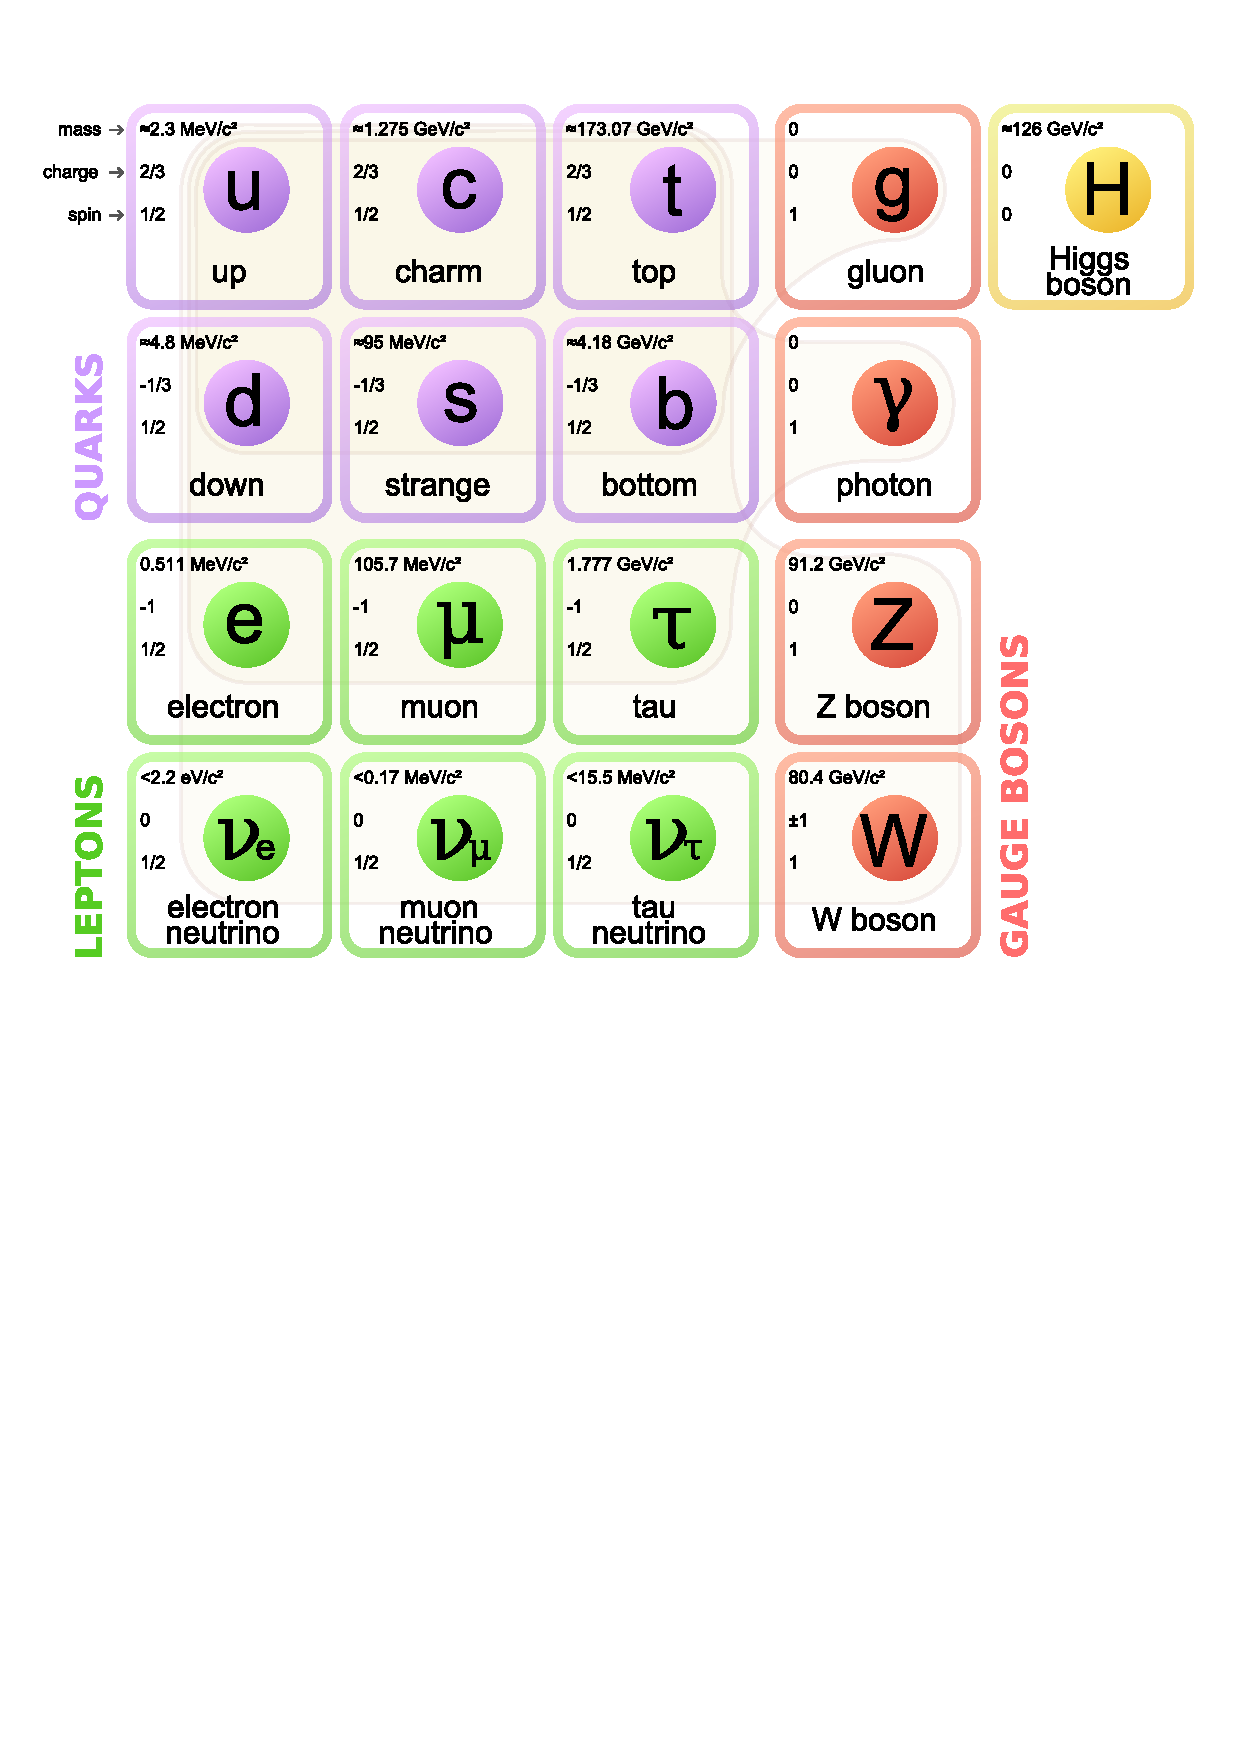
\includegraphics[width=12.cm]{./Version1/FigChapter1/SM}
%\caption{Standard Model families of leptons and quarks as the gauge bosons}
%\label{fig:sm}
%\end{center}
%\end{figure}

%Mathematically, the SM is a quantized Yang-Mills theory based on the non-abelian symmetry group U(1)$\rightarrow$SU(2)$\rightarrow$SU(3) and has a total of twelve gauge bosons: the photon, three weak bosons and eight gluons. The interactions included in such a model are the electromagnetic force, the weak force and the strong one. Quarks have a property called color, playing the role of charge in the strong force. Both quarks and leptons are affected by the weak force and all the charged particles interact electromagnetically.
The models that describe these interactions are listed as follows: \\

\textbf{Quantum Electro-Dynamics (QED)} is a quantum field theory of the electromagnetic force and describes how light and matter interact. This is the first theory where full agreement between quantum mechanics and special relativity is achieved. It explains mathematically not only all interactions of light with matter but also those of charged particles with one another.\\
%It was developed between 1946 and 1950 by Tomonaga Shinichiro, Julian S. Schwinger and Richard P. Feynmann. They were awarded the Nobel prize in 1965. \\

\textbf{Electroweak Theory (EW)} is the unified description of two of the four known fundamental interactions of nature: electromagnetism and the weak interaction. The first measurement of the existence of the weak bosons W$^{+}$, W$^{-}$ and Z$^{0}$ was performed in 1983, when they were produced and directly observed in S$p\bar{p}$S collisions at CERN.\\

\textbf{Quantum Chromo-dynamics (QCD)} is the theory of the strong interaction (color force), describing the interactions between quarks and gluons which make up the hadrons. Starting from the classification of the large amount of particles discovered during the fifties, the original idea of the quark model by Gell-Mann (Nobel Prize in 1969) has been developed during the sixties until 1973, when David J. Gross, H. David Politzer and Frank Wilczek discovered the asymptotic freedom property of the strong nuclear interaction.

\subsection{QCD and Quark-Gloun plasma}\label{label:qcd}
%The strong interaction is one of the four fundamental forces in nature, together with gravity, electromagnetism and the weak interaction. Its existence was postulated in the 1970s, to explain how the atomic nucleus was bound together despite the protons? mutual electromagnetic repulsion. This hypothesized force was called the strong force, which was believed to be a fundamental force that acted on the nucleons. It was later discovered that protons and neutrons were not fundamental particles, by means of deep inelastic experiments, but were made up of constituent particles (the quarks). The strong attraction between nucleons was the side-effect of a more fundamental force that bounds the quarks together in the protons and neutrons. Nowadays the strong inter- action is described through the formalism of a Quantum Field Theory. The particular theory describing this force is the Quantum Chromo-Dynamics (QCD), in analogy to the Quantum Electro-Dynamics (QED) that describes the electromagnetic interaction. In QED the electromagnetic force is mediated by photons, which carry no charge. Similarly, in QCD the gluons are the carriers of the strong force, but unlike the photon they carry color charge, meaning that they can interact with each other. In QED, the electrodynamic coupling constant is $\alpha$ = 1/137, whereas the QCD strong coupling constant, $\alpha_{s}$, can be 1 or larger. In quantum field theory when a coupling constant is much smaller than 1 the theory is said to be weakly coupled. When the coupling nears 1 the theory is strongly coupled, hence the name ?strong? force. In QCD the strong interaction between two quarks can be described using the following potential:
            
As the number of known particle species became large, the idea that these could be the elementary constituents of matter was replaced by the notion that these species could in fact be composite objects made up of fewer, more elementary particles, in a similar way to what had already happened to the elements of Mendeleev's Periodic Table. The original idea by Gell-Mann (1964) was that the hadrons could be obtained as combination of the fundamental representation of an SU$_{f}$(3) group, where three different flavors of quark (q = u, d, s) combine to build mesons ($q\bar{q}$) and hadrons ($qqq$).
However, when cataloging hadrons using the SU$_{f}$(3) group, there are anomalous states, such as the $\Omega^{-}$(sss) and the  $\Delta^{++}$(uuu), that are combinations of three quarks of the same flavor, in clear contrast with the Pauli exclusion principle for fermions. A solution was proposed in 1965 by Moo-Young Han with Yoichiro Nambu and Oscar W. Greenberg, who independently solved the problem by proposing that quarks possess an additional SU(3) gauge quantum number, later called color charge.
This new quantum number may assume three states, represented by the three primary colors: red, green and blue (denoted symbolically by R, G and B, respectively). The introduction of this new quantum number also provides an explanation to other empirical evidence, such as the fact that no $qq$, $\bar{qq}$ or the single quark have never been observed directly. On the other hand, the existence of color charge gives rise to the possible existence of differently colored states for each particle. Thus, we could have many states for the proton, such as u$_{R}$u$_{G}$d$_{B}$, u$_{R}$u$_{G}$d$_{G}$, u$_{B}$u$_{R}$d$_{R}$, and so on. The fundamental rule that solves such contradictions is that all the particle states observed in nature are "colorless" or "white" (or, to be more precise, unchanged under SU$_{c}$(3) rotations).
The dynamics of the quarks and gluons are controlled by the gauge invariant QCD Lagrangian:


\begin{equation}\label{label:L}
\mathcal{L}_{QCD} = \underbrace{i\delta_{ij}\bar{\Psi}^{i}_{q}\gamma^{\mu}\partial_{\mu}\Psi^{j}_{q}}_{\mathcal{L}_{1}}+ \underbrace{g_{s}\bar{\Psi}^{i}_{q}\gamma^{\mu}t_{ij}^{a}A_{\mu}^{a}\Psi^{j}_{q}}_{\mathcal{L}_{2}}+ \underbrace{m_{q}\bar{\Psi}^{i}_{q}\Psi^{j}_{q}}_{\mathcal{L}_{3}}+ \underbrace{\frac{1}{4}F_{\mu\nu}^{a}F^{a \mu\nu}}_{\mathcal{L}_{4}}
\end{equation}

where the coloured gluon field tensor, $F_{\mu\nu}^{a}$ (with color index $a$) and the squared gauge coupling parameter, $g_{s}^{2}$ (associated to the strong coupling constant $\alpha_{s}$) are
defined as:

\begin{equation}\label{label:F}
F_{\mu\nu}^{a} = \partial_{\mu}A_{\nu}^{a} - \partial_{\nu}A_{\mu}^{a} + g_{s}f^{abc}A_{\mu}^{b}A_{\nu}^{c} \end{equation}

and

\begin{equation}\label{label:g}
g_{s}^{2} = 4\pi\alpha_{s}
\end{equation}

where:

\begin{itemize}
\item $\Psi_{q}^{i}$: the quark field with flavor q and color index i $\in$ [1;3], such as $\Psi_{q}$ = ($\Psi_{qR}$, $\Psi_{qG}$, $\Psi_{qB}$)$^{T}$ and $A_{\mu}^{a}$ is the gluon field with color index a (adjoint representation)
\item $\gamma^{\mu}$: Dirac matrices that express the vector nature of the strong interaction, with $\mu$ being the Lorentz vector associated index
\item $m_{q}$: quark mass, a priori not equal to zero (resulting from the Higgs mechanism or equivalent)
\item $t_{ij}^{a}$: generator matrices of the group SU$_{c}$(3), proportional to the Gell-Mann matrices, that perform revolutions in color space, representing interaction of quarks and gluons
\item $f^{abc}$: structure constant of QCD
\end{itemize}

Each of the four terms of the QCD Lagrangian expresses and aspect of the interaction, specifically:

\begin{itemize}
\item $\mathcal{L}_{1}$: gives the kinetic energy of the quark field $\Psi_{q}^{i}$
\item $\mathcal{L}_{2}$: gives the interaction between quarks (fermions) and gluons (the bosons of the interaction)
\item $\mathcal{L}_{3}$: gives the mass of the quarks
\item $\mathcal{L}_{4}$: gives the kinetic energy of the gluons
\end{itemize}

The terms of this equation, together with the fundamental parameters $\alpha_{s}$ and $m_{q}$, summarize in just one expression all the features of the strong interaction. 
The first three terms describe the free propagation of quarks and gluons and the quark-gluon interaction. The remaining two terms show the presence of three and four gluon vertices in QCD and reflect the fact that gluons themselves carry color charge. This is a consequence of the non-abelian4 character of the gauge group.
This peculiarity of the QCD interaction imposes the evolution of the strong coupling constant, $\alpha_{s}$. The corresponding trend has been measured experimentally, and compared in Figure \ref{fig:alpha} with predictions. A practical consequence of this behavior is that the corresponding potential has a completely different shape than the other fundamental interactions and can be expressed by the following equation:


\begin{equation}\label{label:potential}
V(r) = -4\frac{\alpha_{s}}{3r} + kr
\end{equation}

where r is the separation distance between the two quarks and $k$ is a constant that is approximately 1 GeV/fm. %The renormalization scale dependence of the effective QCD coupling $\alpha_{s}$ = $g^{2}_{s}$/4$\pi$ is controlled by the $\beta$-function:

\begin{figure}[htbp]
\begin{center}
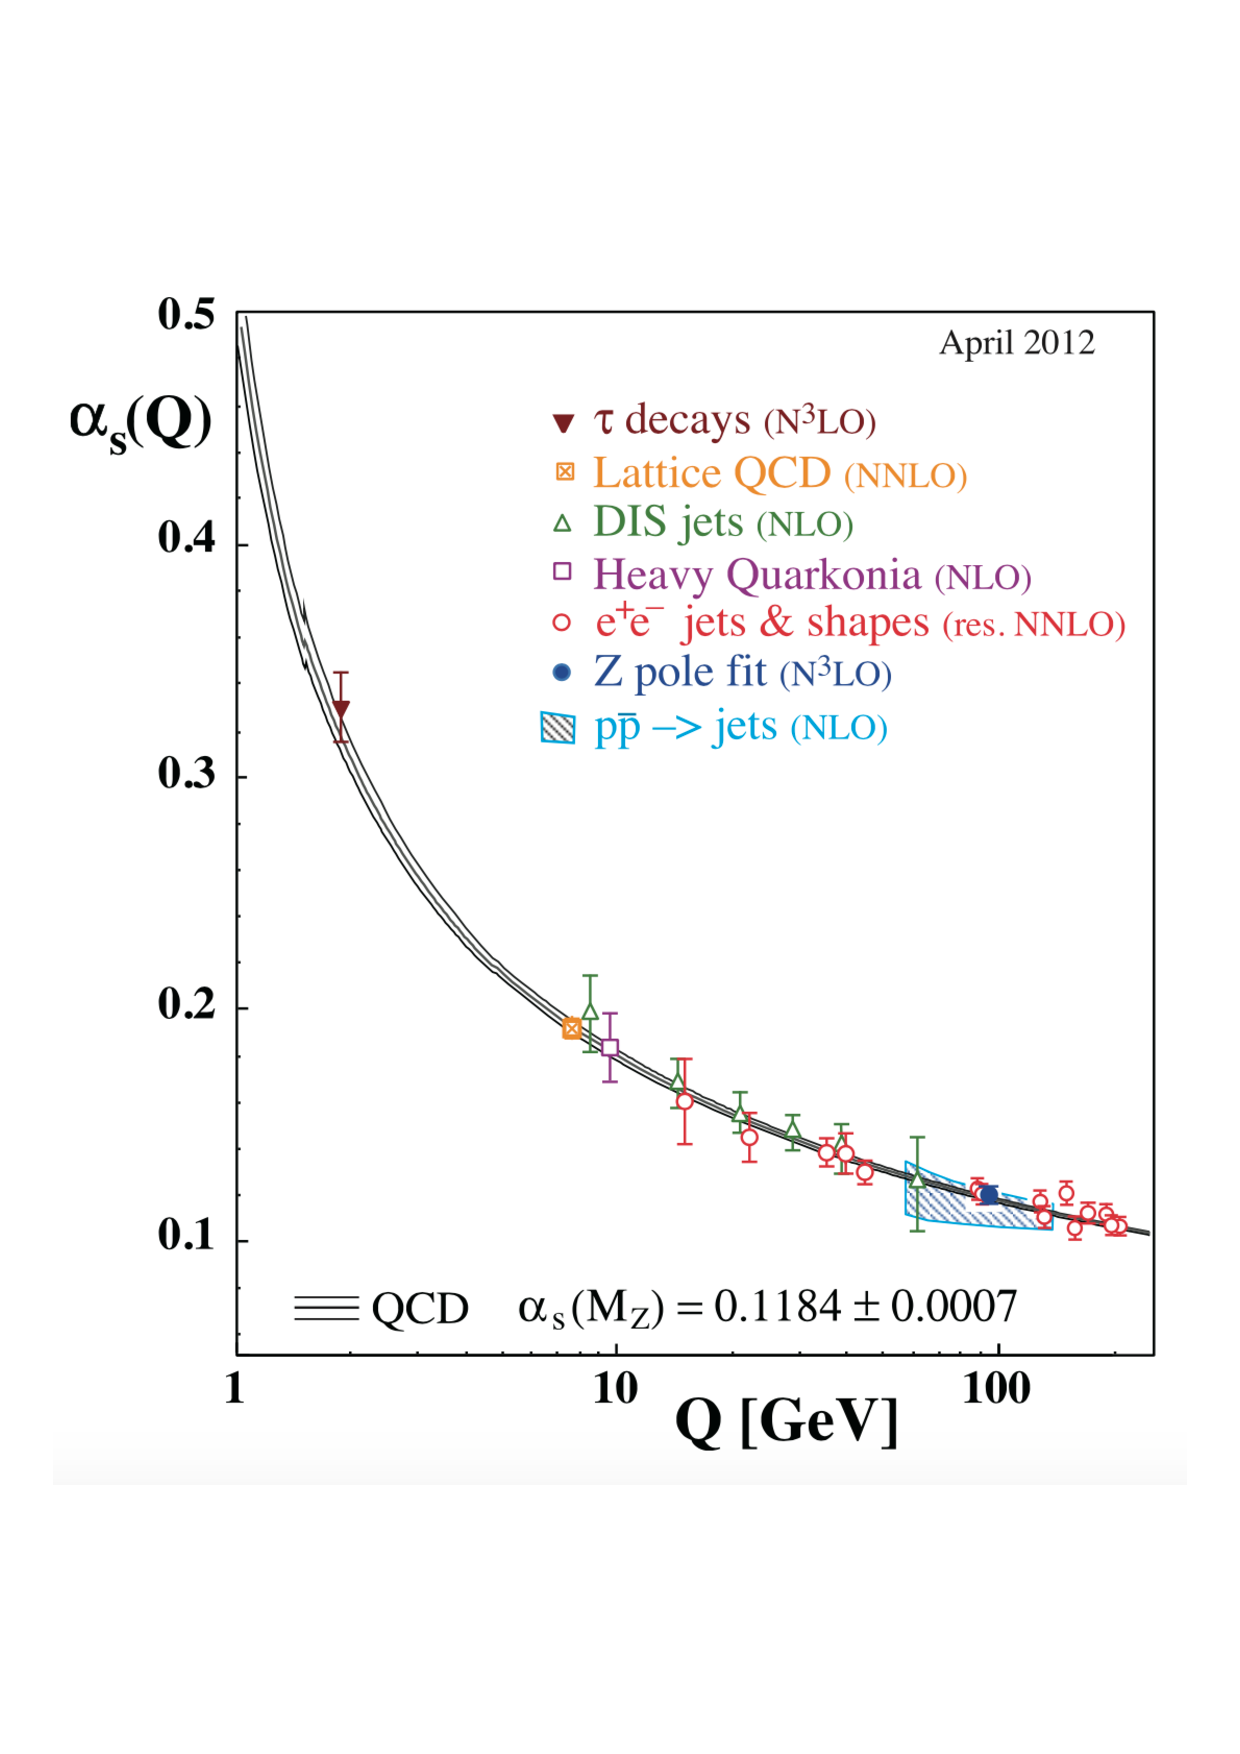
\includegraphics[width=12.cm]{./Version1/FigChapter1/QCD_alpha}
\caption{QCD coupling constant as a function of momentum transfer. Experimental data and also theoretical prediction are presented. \cite{cite:PDG}}
\label{fig:alpha}
\end{center}
\end{figure}

Three are main properties of the QCD interaction: \\

\textbf{Confinement}
At large distances between quarks and gluons (i.e. small values of transferred momentum $Q$ in Figure \ref{fig:alpha}) the coupling constant is large and the associated force is strong enough to keep these elementary con- stituents (usually called partons) confined in bounded states. As expressed in the Equation \ref{label:potential}, the attractive potential increases with the increasing of the relative distance between the two partons preventing the separation of an individual quark or gluon. This explains the meaning of the term "confinement" adopted to describe this energy regime. From the theoretical point of view, the large value of $\alpha_{s}$ make impossible any perturbative approach in the solution of the Hamilton equation of the system. A successful solution is to perform the study of the system on a discrete space. Such techniques are known as lattice QCD and are based on numerical Monte Carlo simulations. The challenge for the calculations is to reduce the lattice spacing in order to approach the continuum.\\

\textbf{Asymptotic freedom}
Reducing the distance between quarks and gluons (i.e. increasing $Q$ in Figure \ref{fig:alpha}) the coupling constant $\alpha_{s}$ becomes smaller. As anticipated, this is a unique feature among the forces and comes from the non-abelian nature of the QCD gauge symmetry. Such a phenomenon is also depicted by the weakening of the anti-screening effect of the surround- ing virtual gluons with decreasing distance. In this way two quarks closer and closer in space show each other a smaller and smaller color charge. \\


\textbf{Chiral symmetry}
One further property of interest is connected to the chirality of the quark. It can be verified that the QCD lagrangian for massless quarks is invariant under a chiral rotation (SU$_{L}$(N$_{f}$) $\times$ SU$_{R}$(N$_{f}$)), while the operator $\bar{q}$q = $\bar{q}_{L}$q$_{R}$ + $\bar{q}_{R}$q$_{L}$ is not invariant (in the axial part), meaning that the mesons (state $\bar{q}$q) should have the same mass. Experimentally this is clearly not true, and it could be shown that the axial current is conserved (PCAC and the Goldberger-Treiman relation). The solution to this puzzle is that the chiral (axial-vector) symmetry is spontaneously broken; this means that the symmetry of the Hamiltonian is not a symmetry of the corresponding ground state. It has also been shown, by G. t?Hooft, that the confinement implies a dynamical breaking of the chiral symmetry. This means that the breaking comes from the interaction between the objects in the system. From this follows that the masses of the quarks are strongly increased because of the interaction with the constituents of the system. This mechanism, known as dynamical chiral symmetry breaking justifies the mass of the hadrons, reducing the role of the Higgs mechanism in the mass explanation at least for the light hadrons.


The asymptotic freedom property suggests the existence of a state of matter, called Quark-Gluon Plasma (QGP), in which the constituents of the hadrons are de-confined. The hatched region in Figure \ref{fig:phase} presents the expected phase boundary between partonic and hadronic matter from lattice QCD calculations. 

Two relevant thermodynamical observables of the system are plotted in the figure. One is temperature T and another one is the baryonic chemical potential $\mu_{B}$. The red points have been measured from thermal models fit on data from different experiment \cite{cite:thermal_pbm} and lie along a line that represent the limit between the two phases. As one can see in Figure \ref{fig:phase}, there are different ways to achieve the transition. It can be performed by changing the temperature and/or the net baryonic density ($\mu_{B}$). 

\begin{figure}[htbp]
\begin{center}
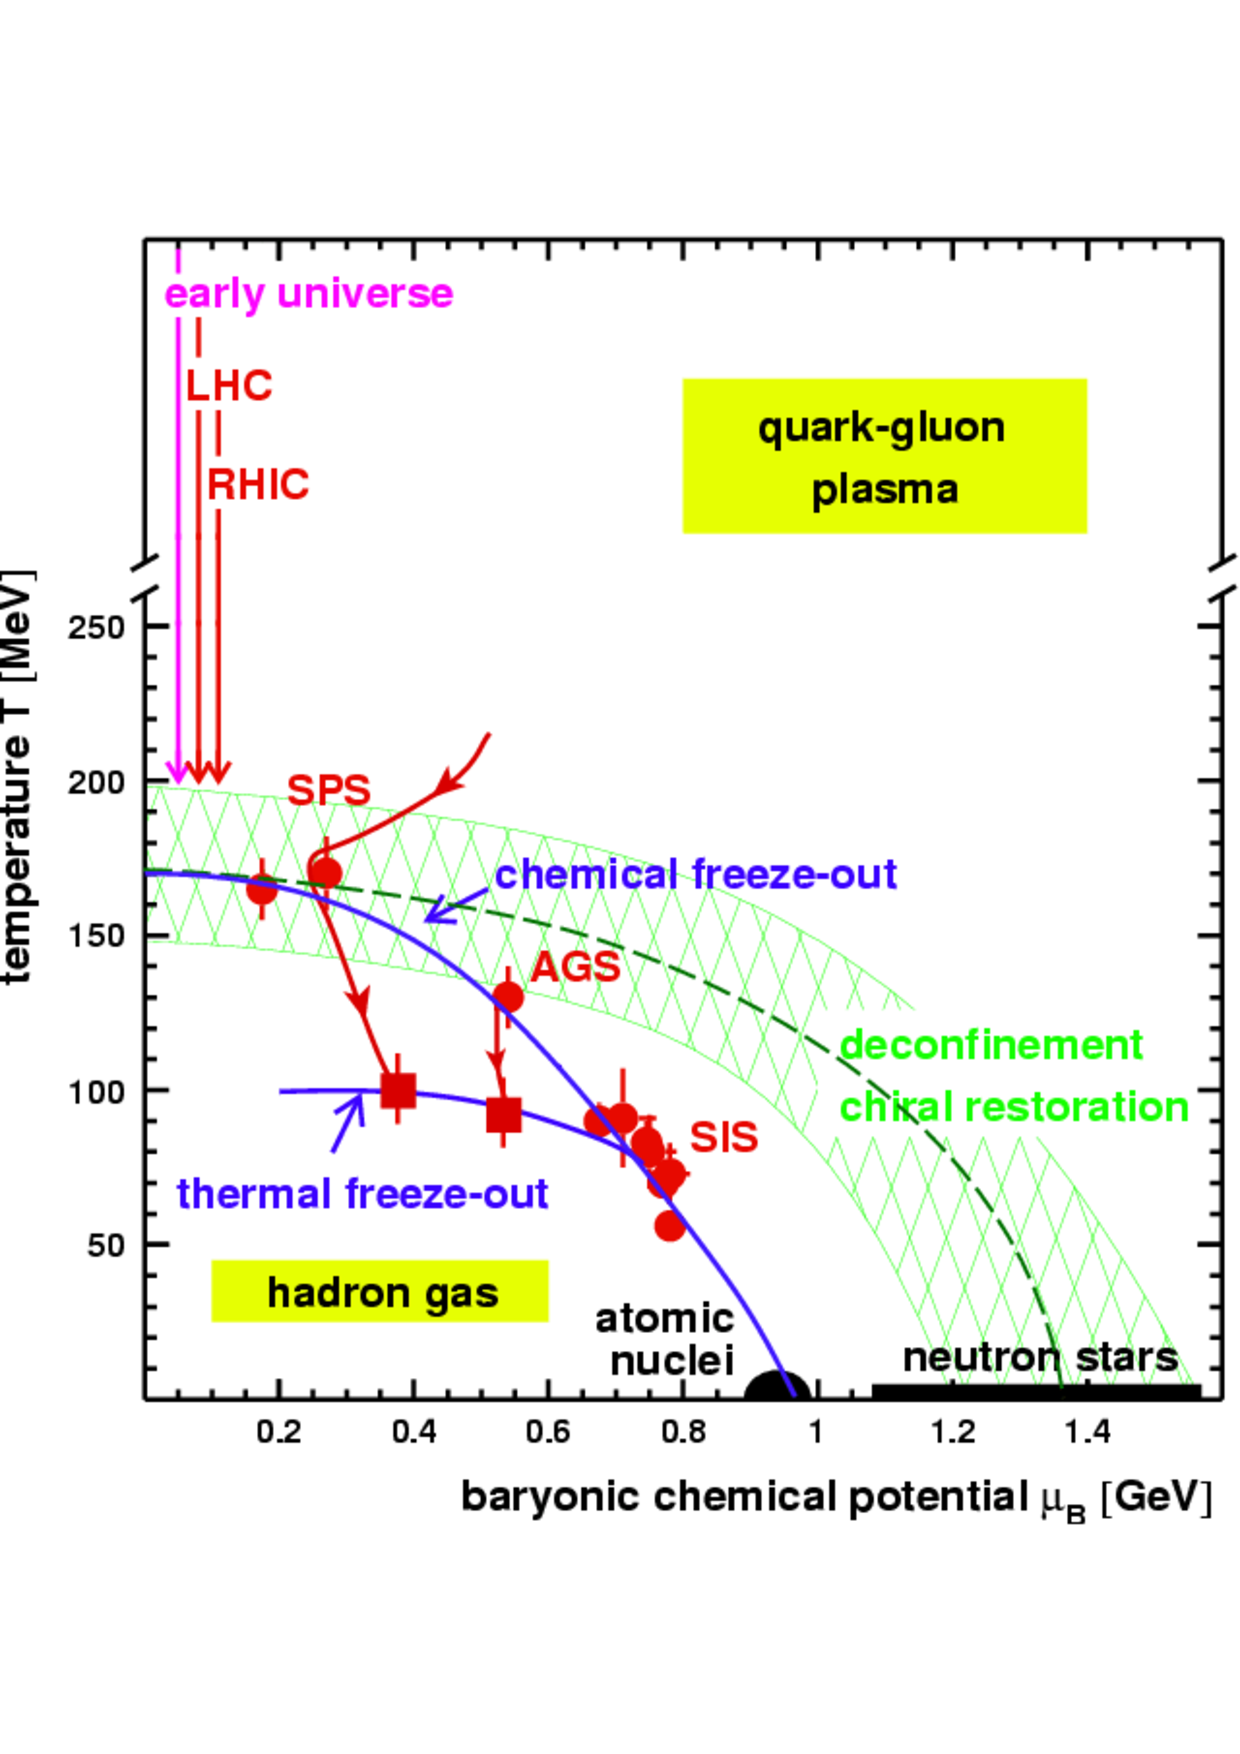
\includegraphics[width=12.cm]{./Version1/FigChapter1/PhaseDiagram}
\caption{Phase diagram of partonic and hadronic matter. The chemical freeze out points are determined from thermal models fit to heavy ion data at SIS, AGS, and SPS energies. (http://na49info.web.cern.ch/na49info/Public/Press/findings.html)}
\label{fig:phase}
\end{center}
\end{figure}


%Experimentally, $\alpha_{s}$ has been measured at different scales ($\mu$). Figure \ref{fig:alpha} shows the measurement of $\alpha_{s}$ as a function of the respective energy scale $Q$ compared to the lattice QCD calculation. Three very important properties of QCD arise from the running constant $\alpha_{s}$. They are confinement, asymptotic freedom, and (hidden) chiral symmetry. For large distance scales the second term in the potential equation (Equation \ref{label:expansions}) dominates. This means that the coupling between the two quarks is large, making it so that no free quarks are observed in nature, i.e. a quark never exists on its own for longer than 1/$\Lambda$QCD, where $\Lambda$QCD = 217 MeV. The up, down, strange, charm, and bottom quarks all hadronize on the time-scale 1/$\Lambda$QCD, the top quark decays before it has time to hadronize. Therefore, all but the top quark will be confined inside hadrons. Experimentally, no single quark in a color- triplet state has ever been observed. Asymptotic freedom arises when the quarks are at a small distance from one another or with a large enough momentum transfer $Q$ ($\alpha_{s}$ $\rightarrow$ 0 as $\mu$ $\rightarrow$ $\infty$). The potential will go like 1/r and the effective coupling between the quarks decreases, allowing for a quasi-free quark. The third property is called chiral symmetry, also not observed in nature. It is a symmetry of QCD in the limit of vanishing quark masses. In this limit quarks are either left of right handed, such that the QCD Lagrangian is symmetric. However, when quarks are confined inside hadrons they have large dynamical masses, called constituent or QCD masses. Here the chiral symmetry is said to be ?broken? (or hidden). In the small ?s limit some quarks will have small mass, called current mass. In this limit, chiral symmetry is said to be (partially) restored. In our world, quarks and gluons are confined inside hadrons. By significantly increasing the temperature and energy density the strong force holding the quarks and gluons together may be reduced, unbinding them from the hadrons. This phenomenon is known as "de-confinement". De-confinement implies that there exists a phase transition from a gas of hadrons to a new form of matter of free quarks and gluons, called the Quark-Gluon Plasma (QGP).

\newpage
\subsection{Heavy Ion Collisions}

Knowledge of the space-time evolution of the system created in high energy heavy ion collisions help to understand the dynamics of nuclear matter under extreme conditions. 
The Figure \ref{fig:HI} presents the schematic of the time evolution in case of collision of two Lorentz contracted nuclei at very high energy. After the colliding, a large amount of energy can be deposited in a small area of space and in a short duration of time. The matter produced might have very high energy density and temperature so that it is sufficiently able to reach to QGP that is baryon free region.

Just after the colliding, the medium may not be in thermal equilibrium which can be reached after that the evolution is governed by the low of thermodynamics. As the system expands and cools, the hadronization takes place and and the freeze out comes after some time.
Different stages during the collisions can be studied by various observables, such as, Electromagnetic probes,  Quarkonia and heavy flavour, Hard probes, Electroweak probes, global properties and Freeze-out condition as well. Most of the produced particles in the high energy heavy-ion collisions are emitted at freeze-out. In order to estimate the energy density, pressure, temperature and baryon chemical potential, the study of particle after freeze-out gives crucial information. Those quantities could be derived from measurement of multiplicity and rapidity distribution, transverse momentum (\pt) distributions.


\begin{figure}[htbp]
\begin{center}
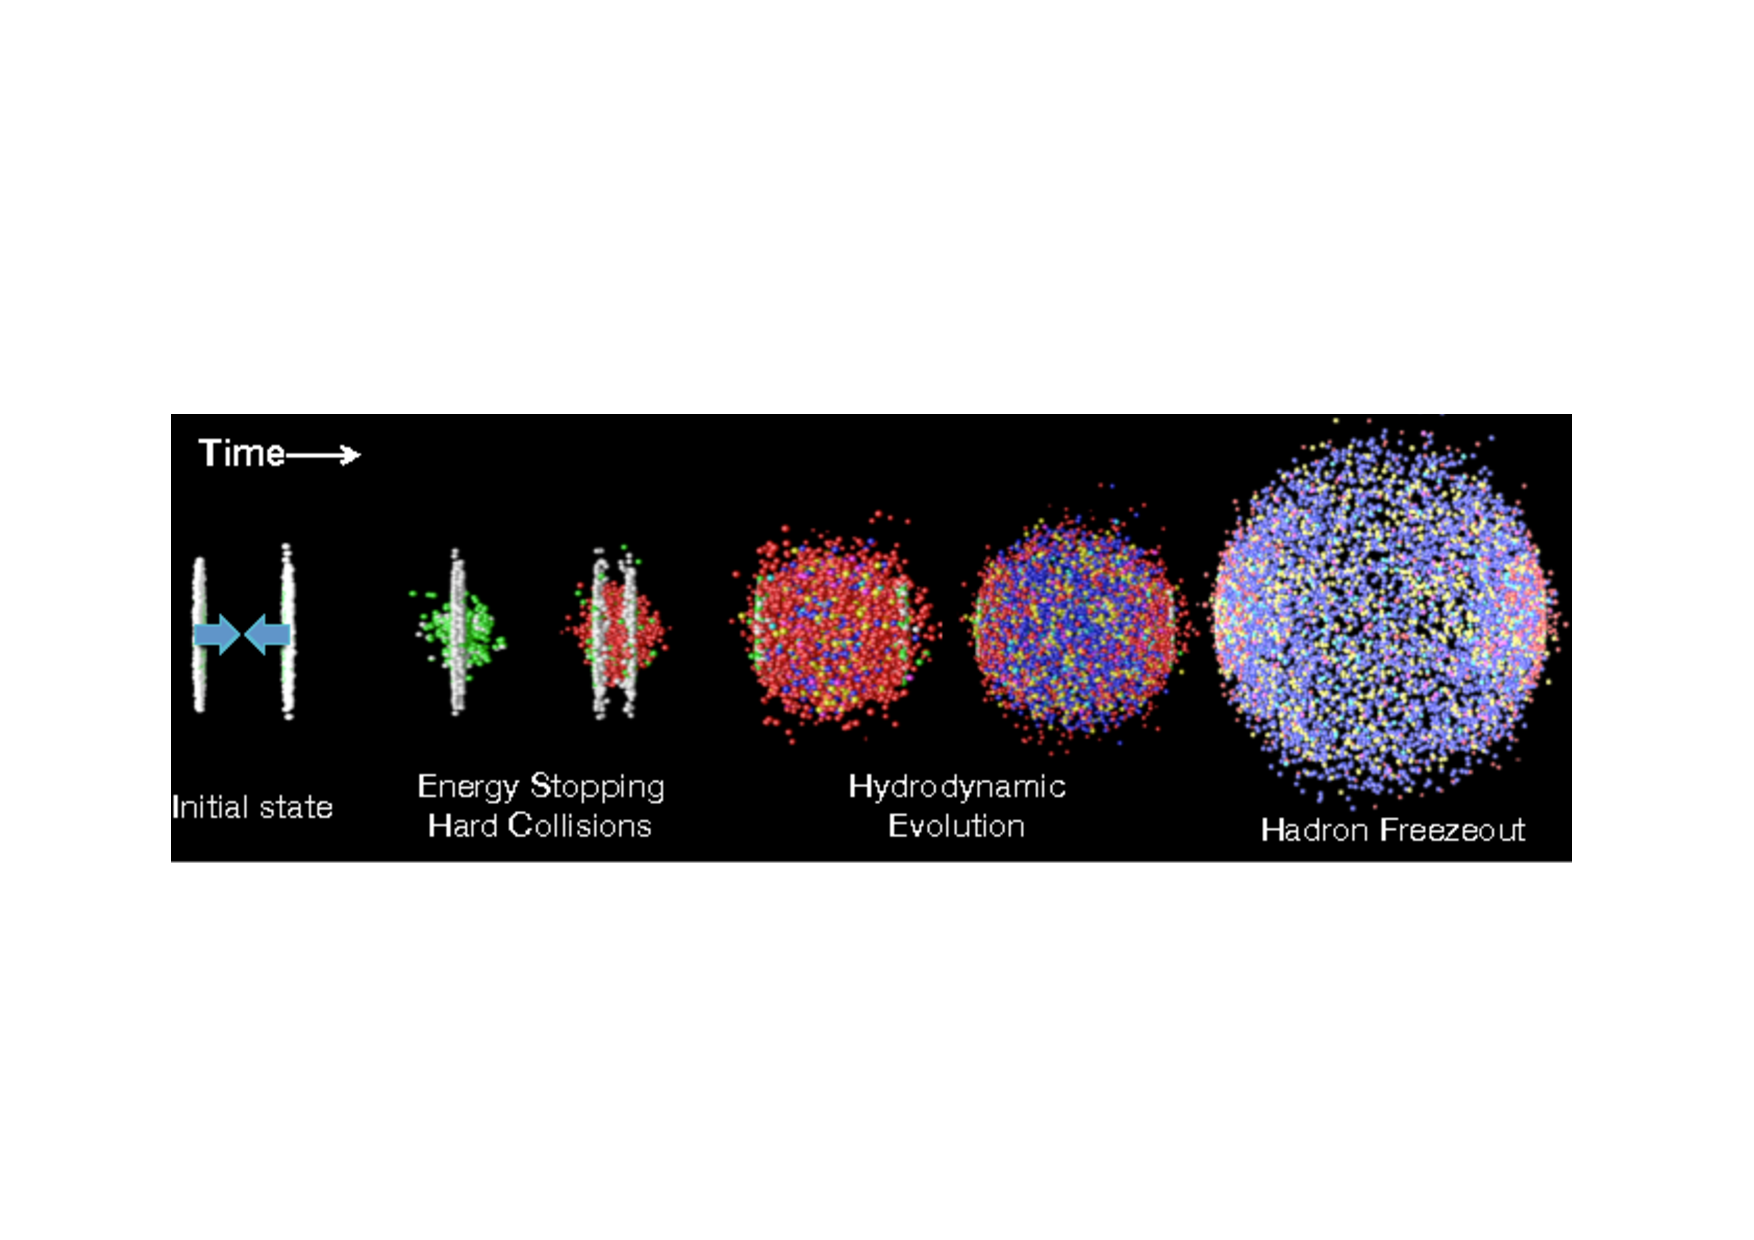
\includegraphics[width=12.cm]{./Version1/FigChapter1/HI}
\caption{The time evolution of a high energy heavy ion collision. \cite{cite:HI}}
\label{fig:HI}
\end{center}
\end{figure}

In the case a QGP is formed, it will eventually expand because of its internal pressure. As the system expands it also cools. The space-time evolution of the expansion can be seen in Figure \ref{fig:freezeout} (right side). A and B represent the two incoming ion beams. After a pre- equilibrium phase a QGP is formed. As it expands, the system will eventually reach what is known as the critical temperature ($T_{c}$). At this point partons begin to hadronize and this will continue until the chemical freeze-out ($T_{ch}$) takes place, when inelastic collisions cease. At this stage the distribution of hadrons is frozen. As cooling and expansion continue the hadrons reach what is called thermal freeze out ($T_{fo}$). Here the elastic collisions stop and the hadrons carry fixed momenta. The QGP state can not be directly observed, because of its short lifetime. Instead, through experiment we measure the final state hadrons, which have a fixed momentum after $T_{fo}$. The observables of interest should tell us about the de-confinement and the thermodynamic properties of the matter. Moreover, experimental measurements include yields and \pt spectra of various particle species, azimuthal studies of high \pt particles, phase space distributions, and particle correlations.

\begin{figure}[htbp]
\begin{center}
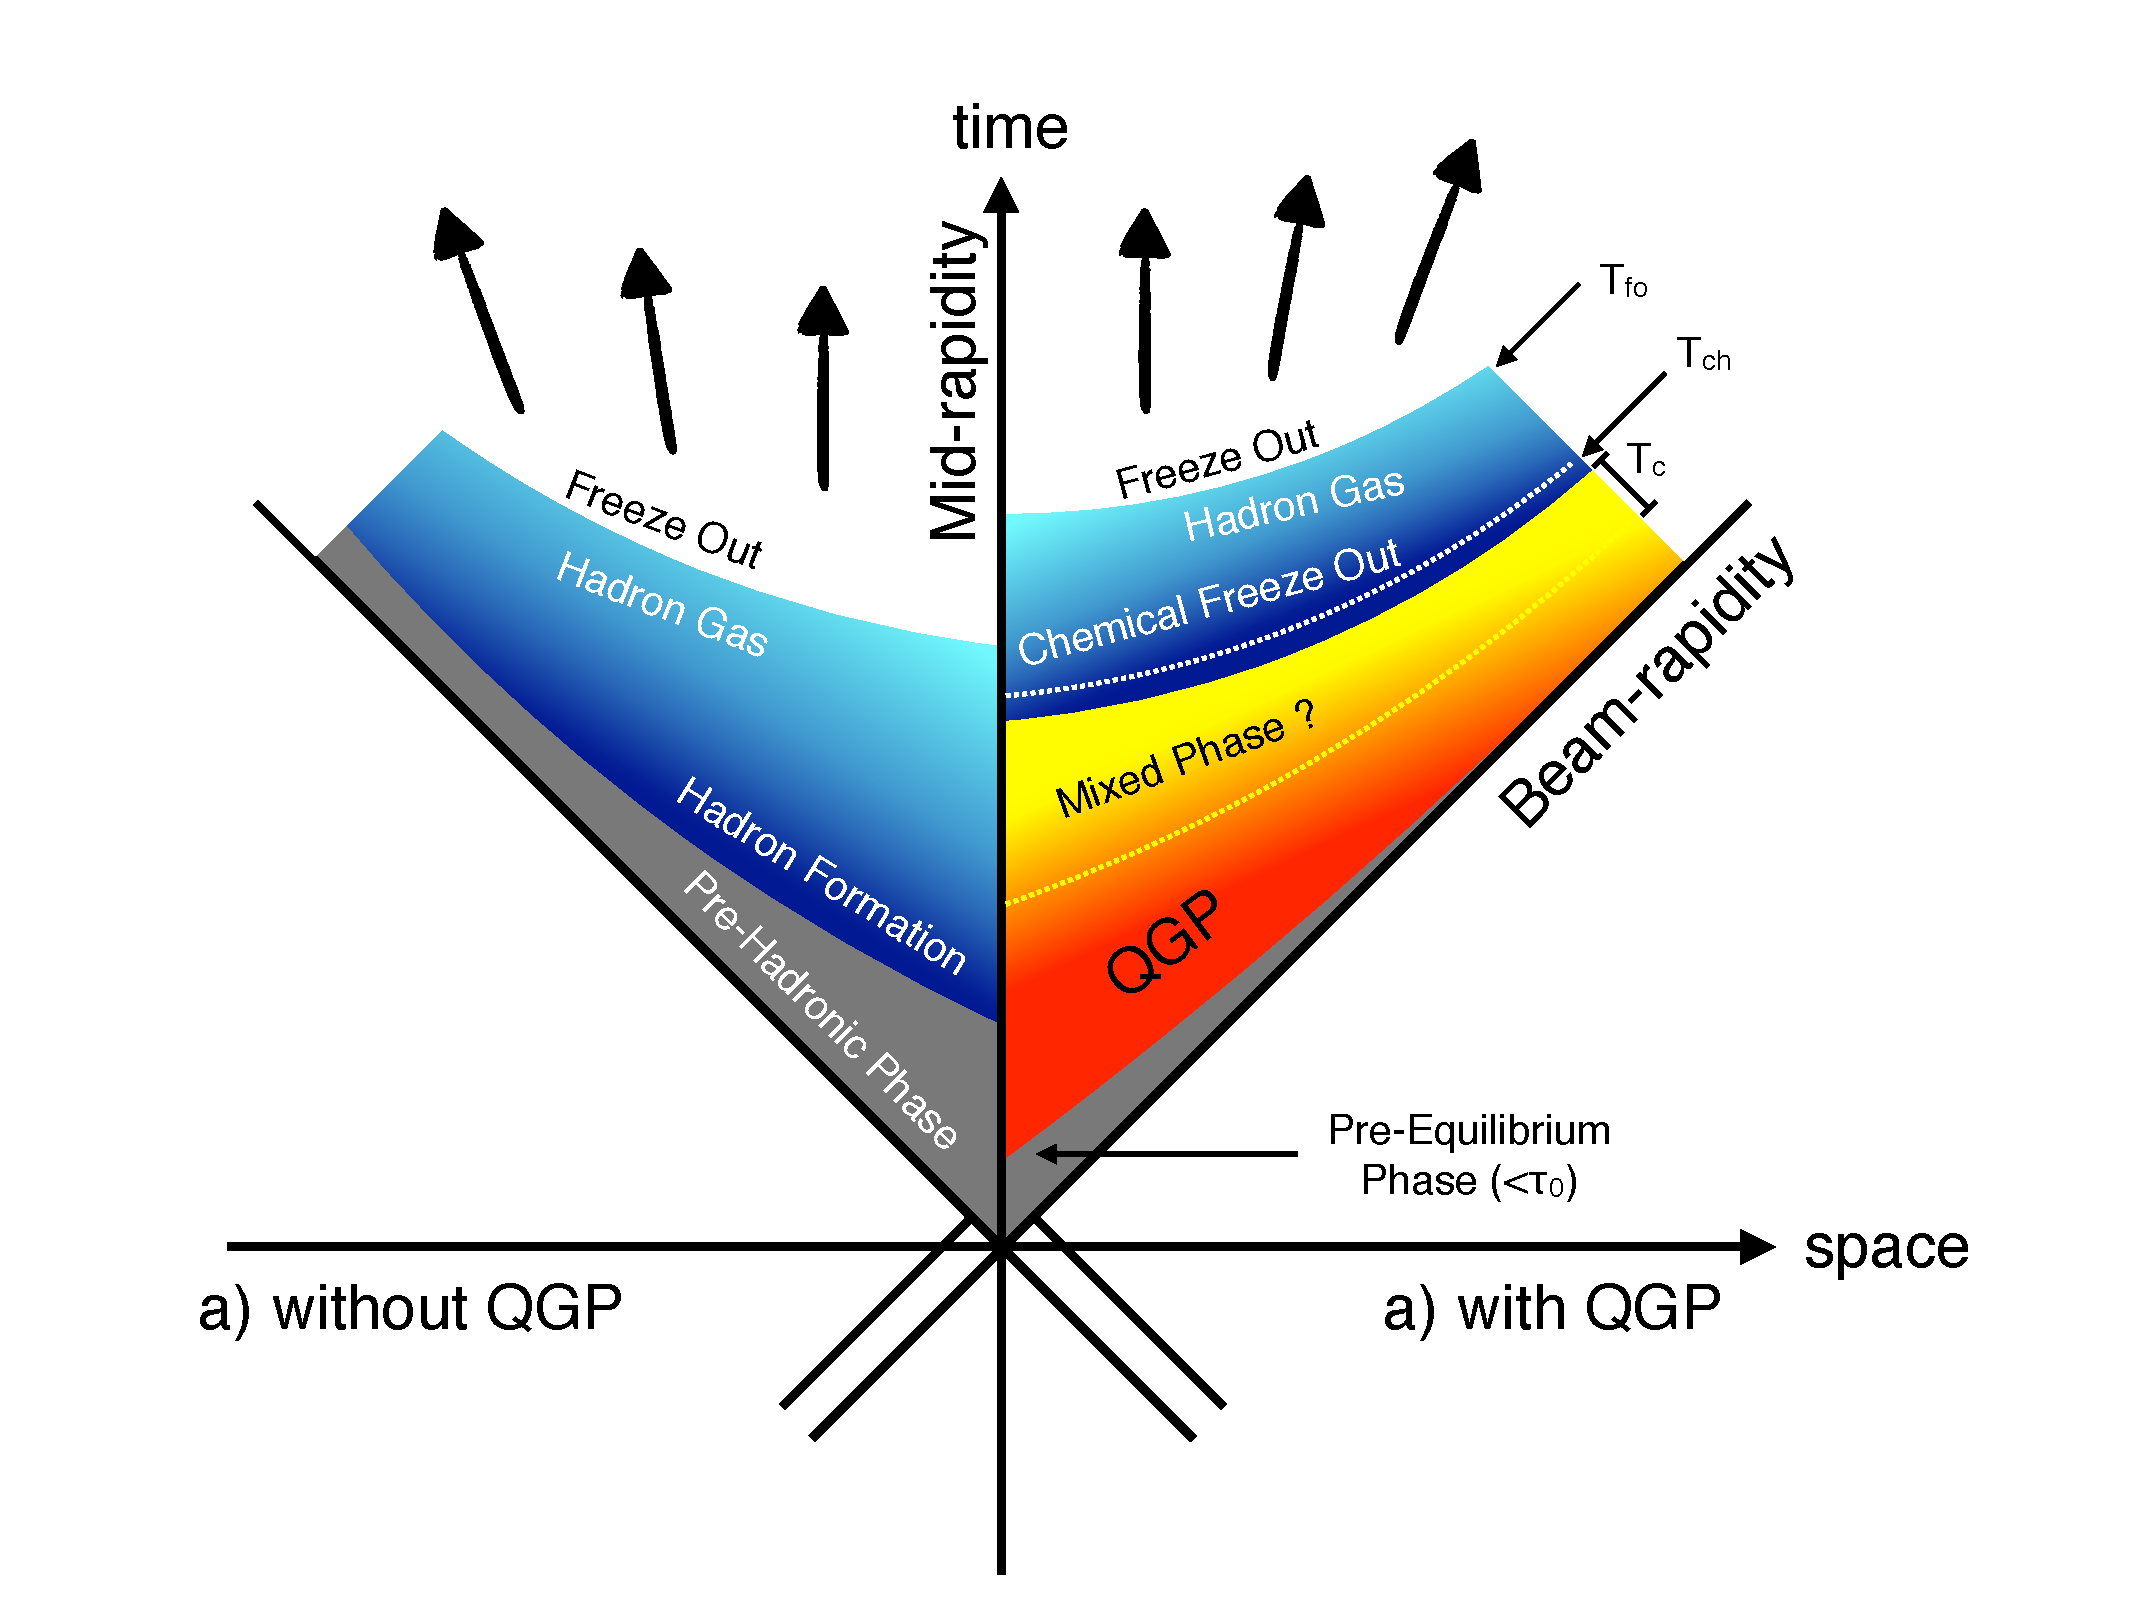
\includegraphics[width=18.cm]{./Version1/FigChapter1/FreezeOut}
\caption{Hydrodynamic evolution of a heavy ion collision with and without the formation of a QGP. }
\label{fig:freezeout}
\end{center}
\end{figure}

A practical way to reach a critical condition in which a nuclear system should undergo a phase transition to the QGP, at high temperature and/or matter density, is to collide two nuclei at sufficiently high energy. Therefore, relativistic and ultra-relativistic heavy-ion collisions are a unique tool to study nuclear matter under extreme conditions.



%Three snapshots illustrating a nuclear collision of two nuclei. (Left frame) The two incident nuclei are Lorentz contracted as the incident velocities are already close to the speed of light. (Middle frame) The moment of highest compression. (Right frame) The expansion stage, when most of the particles already no longer interact strongly.


\newpage
%\section{The physics of relativistic heavy-ion collisions}
%\subsection{Standard model}
%\subsection{Quantum Chromo-Dynamics}
%\subsection{Heavy Ion Collisions}

\section{Theoretical models}\label{sec:model}
\subsection{Thermal statistical model}

The statistical-thermal model has proved extremely successful in applications to relativistic collisions of both heavy ions and elementary particles as shown in Figure \ref{fig:thermal}. In light of this success, THERMUS, a thermal model analysis package, has been developed for incorporation into the object-oriented ROOT framework \cite{Wheaton:2004qb}.\\ 

\begin{figure}[htbp]
\begin{center}
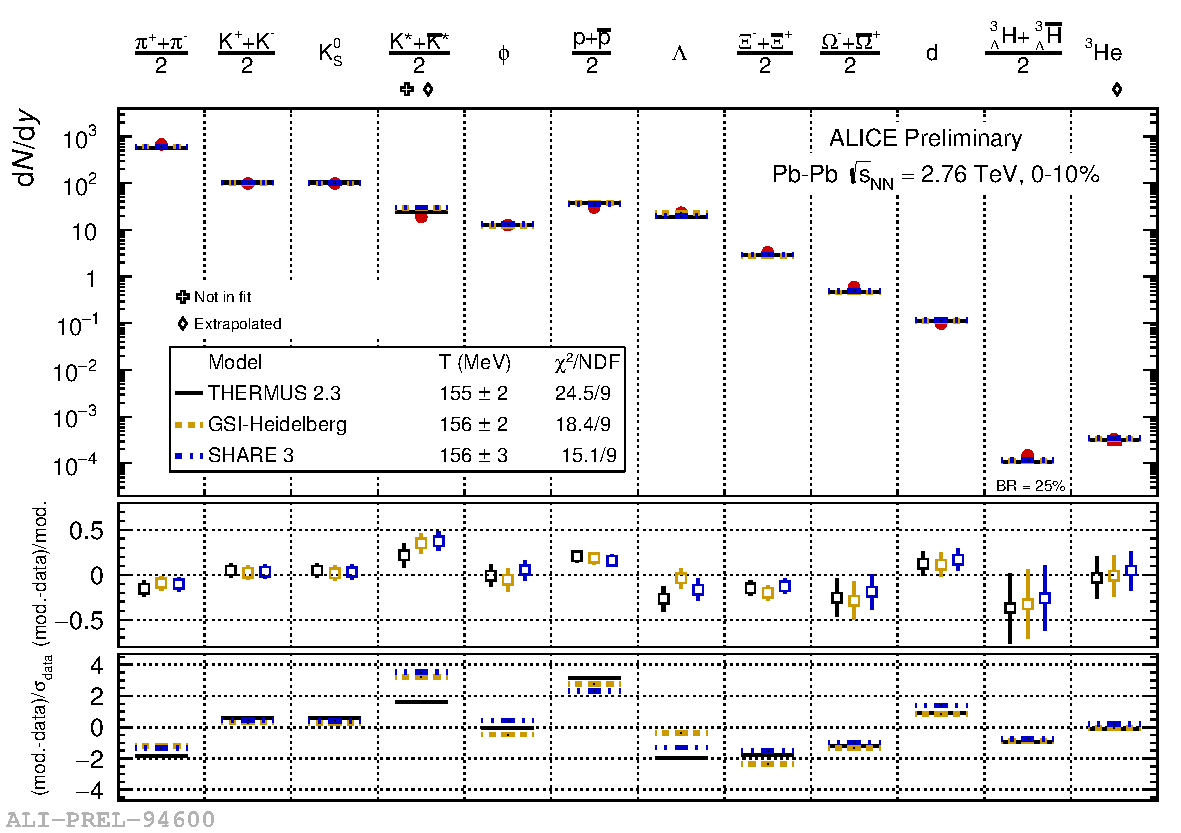
\includegraphics[width=14.cm]{./Version1/FigChapter2/ThermalModel}
\caption{Grand canonical thermal fit of 0-10\% central Pb-Pb collisions, with 3 models (THERMUS, GSI, SHARE). Excluded volume correction implemented in THERMUS and GSI with rh = 0.3 fm $\mu_{B}$ fixed to 0, $\gamma_{s}$ fixed to 1, $\gamma_{c}$ fixed to 20 (THERMUS and GSI)}
\label{fig:thermal}
\end{center}
\end{figure}


There are three types of statistical-thermal models in explaining data in high energy nuclear physics and THERMUS treats the system quantum numbers B (baryon number), S (strangeness) and Q (charge) within three distinct formalisms: 

\begin{enumerate}
\item \textbf{Grand-Canonical Ensemble:} Because the hot dense matter produced in nucleus-nucleus collisions is large enough, this ensemble is the most widely used in applications to heavy-ion collisions, in which the quantum numbers are conserved on average. 
\item \textbf{Fully-Canonical Ensemble:} In which B, S and Q are each exactly conserved and this ensemble used in high-energy elementary collisions such as pp, p\pbar{} and e$^{-}$e$^{+}$ collisions.
\item \textbf{Strangeness-Canonical Ensemble:}  In small systems or at low temperatures, a canonical treatment leads to a suppression of hadrons carrying non-zero quantum numbers, since these particles have to be created in pairs and the resulting low production of strange particles requires a canonical treatment of strangeness.  
 \end{enumerate}
 In order to calculate the thermal properties of a system, one starts with an evaluation of its partition function. The form of the partition function obviously depends on the choice of ensemble. In the present analysis the strangeness-canonical ensemble used and the statistical-thermal model requires six parameters as input: the chemical freeze-out temperature $T$, baryon and charge chemical potentials $\mu_{B}$ and $\mu_{Q}$ respectively, canonical or correlation radius, $R_{C}$; the radius inside which strangeness is exactly conserved and the fireball radius $R$. An additional strangeness saturation factor $\gamma_{S}$ has been used as indicator of a possible departure from equilibrium and $\gamma_{S}=1.0$ corresponds to complete strangeness equilibration.
 

The volume dependence cancels out when studying the particle ratios as well as strangeness canonical equivalent to grand canonical formalism if $\Delta S=0$ in the ratios and $\gamma_{S}$ also cancels out. Parameters used in the analysis listed in Table~\ref{jfonts}. The $\mu_{B}$ parameter taken from the Ref.~\cite{Cleymans:2011pe}.
 
 \begin{center}
\begin{table}[h]
\centering
\caption{\label{jfonts} Parameters used in the thermal-model calculations.} 
%\begin{tabular}{@{}l*{15}{l}}
 \begin{tabular}{@{}*{2}{cc}}
\hline
Parameter&Value\\
\hline
$T$ (MeV)&varied (see text)\\
$\mu_{B}$ (MeV)&$9.2\times10^{-2}$????\\ 
$\mu_{Q}$ (MeV)&$0.0$\\ 
$\gamma_{S}$&$1.0$\\ 
%$R_{C}$ (fm)&$1.5$\\ 
%$R$ (fm)&$4.0$\\ 
\hline
\end{tabular}
\end{table}
\end{center}
\newpage
\subsubsection{Calculations}
\textit{Concept:} \\In order to calculate the particle ratios within strangeness canonical formalism of THERMUS, temperature varied between 60 MeV to 180 MeV and particle yields extracted for each temperature value and then primary particle ratios calculated for each case. \\ \\
\textit{Feed-Down Correction:} \\Since the particle yields measured by the detectors in collision experiments include feed-down from heavier hadrons and hadronic resonances, the primordial hadrons are allowed to decay to particles considered stable by the experiment before model predictions are compared with experimental data. In the analysis only  $\Lambda$ particles counted as stable (do not allowed to decay) so there is no feed-down contribution from these particles to the other ratios.  \\ \\

Properties of studied particles and their particle ratios listed in Table~\ref{opt} and Table~\ref{diff}, respectively. 
%\begin{landscape}

%\begin{center}
%\begin{table}[h]
\hspace*{-1cm}
\begin{table}[!htb] 
\hspace*{-1cm}
%\vspace{1.5 cm}
\caption{\label{opt} Properties of particles used in the ratio calculations.}
%
\hspace*{-1cm}
%
%\addtolength{\tabcolsep}{-2.7pt}
 \begin{tabular}{lcccccccccccc}
\hline
\hline
Particle&$\Delta^{++}$ &  p & K$^{*0}$ &K$^{0} $ &K$^{+} $ & $\Lambda^{*}$ & $\Lambda$& $\Sigma^{*+}$  & $\Sigma^{+}$ & $\Sigma^{0}$ & $\Xi^{*0}$ & $\Xi^{-}$\\
\hline
Mass (MeV/$c^{2}$)&1232&938.27&895.92&497.61&493.67&1519.5&1115.68&1382.8&1189.37&1192.64&1531.80&1321.31\\
%\hline 
Width (MeV/$c^{2}$)&120&--&50.7&--&--&15.6&--&37.6&--&--&9.1&--\\
%\hline
$c\tau$ (fm)&1.6&--&3.9&--&--&12.6&--&5.51&--&--&$21.6$&--\\
%\hline
Ang. Momentum ($J$)&3/2&1/2&1&1&0&3/2&1/2&3/2&1/2&1/2&3/2&1/2\\
%\hline
Isospin ($I$)&3/2&1/2&1/2&1/2&1/2&0&0&1&1&1&1/2&1/2\\
%\hline
Parity ($P$)&+1&+1&-1&-1&0&-1&+1&+1&+1&+1&+1&+1\\
%\hline
Strangeness ($S$)&0&0&1&1&1&-1&-1&-1&-1&-1&-2&-2\\
%\hline
Baryon Number ($B$)&1&1&0&0&0&1&1&1&1&1&1&1\\
%\hline
Decay Channel&p$\pi^{+}$&--&$\pi^{-}$&--&$\mu^{+}\nu_{\mu}$&pK$^{-}$&$p\pi^{-}$&$\Lambda\pi^{+}$&p$\pi^{0}$&$\Lambda\gamma$&$\Xi^{-}\pi^{+}$&$\Lambda\pi^{-}$\\
%\hline
Branching Ratio (\%)&$\sim100$&--&$\sim66.7$&--&$\sim63.54$&$\sim45$&$\sim63.9$&$\sim87$&$\sim51.6$&$\sim100$&$\sim64$&$\sim99.9$\\
Q-Value(MeV/$c^{2}$)&154.16&--&262.68&--&--&87.55&37.84&127.55&111.53&76.96&70.92&70.66\\
 \hline
 \hline
\end{tabular}
\end{table}
%\end{center}

\vspace{6pt}
 \begin{center}
\begin{table}[!htb] 
\caption{\label{diff} Difference of mass ($\Delta M$), baryon number ($\Delta B$), strangeness ($\Delta S$) and charge ($\Delta Q$) of the ratios. The values of the slopes needs to be checked!!!!}
\centering
 \begin{tabular}{lcccccccc}
 	 		\hline
\hline
Particle&$\Delta^{++}$/p & K$^{*}$/K$^{+}$& $\Lambda^{*}/\Lambda$&$\Sigma^{*+}/\Lambda$  &$\Sigma^{*+}/\Sigma^{0}$ &$\Sigma^{0}/\Lambda$ & $\Sigma^{*+}/\Sigma^{+}$ & $\Xi^{*0}/\Xi^{-}$\\
\hline
\textit{$\Delta M$ ({\rm MeV}/$c^{2}$)}&293.8&402.25&403.82&267.12&190.16&76.96&193.43&210.49\\
\textit{$\Delta B$}&0&0&0&0&0&0&0&0\\
\textit{$\Delta S$}&0&0&0&0&0&0&0&0\\
\textit{$\Delta Q$}&+1&-1&0&+1&0&+1&0&-1\\
%\textit{Q-Value ($MeV/c^{2}$)}&154.16&262.68&87.55&87.55&127.55&127.55&76.96&127.55&70.92\\
\hline
Slope (\%) per MeV ??????& 0.19 &0.76& 0.98& 0.25 & - & -0.08 &0.37 &0.42\\
 \hline
\end{tabular}
\end{table}
\end{center}
%\end{landscape}

%\newpage	

\subsubsection{Results and comparison with data}
\begin{figure}[!htbp]
\begin{center}
        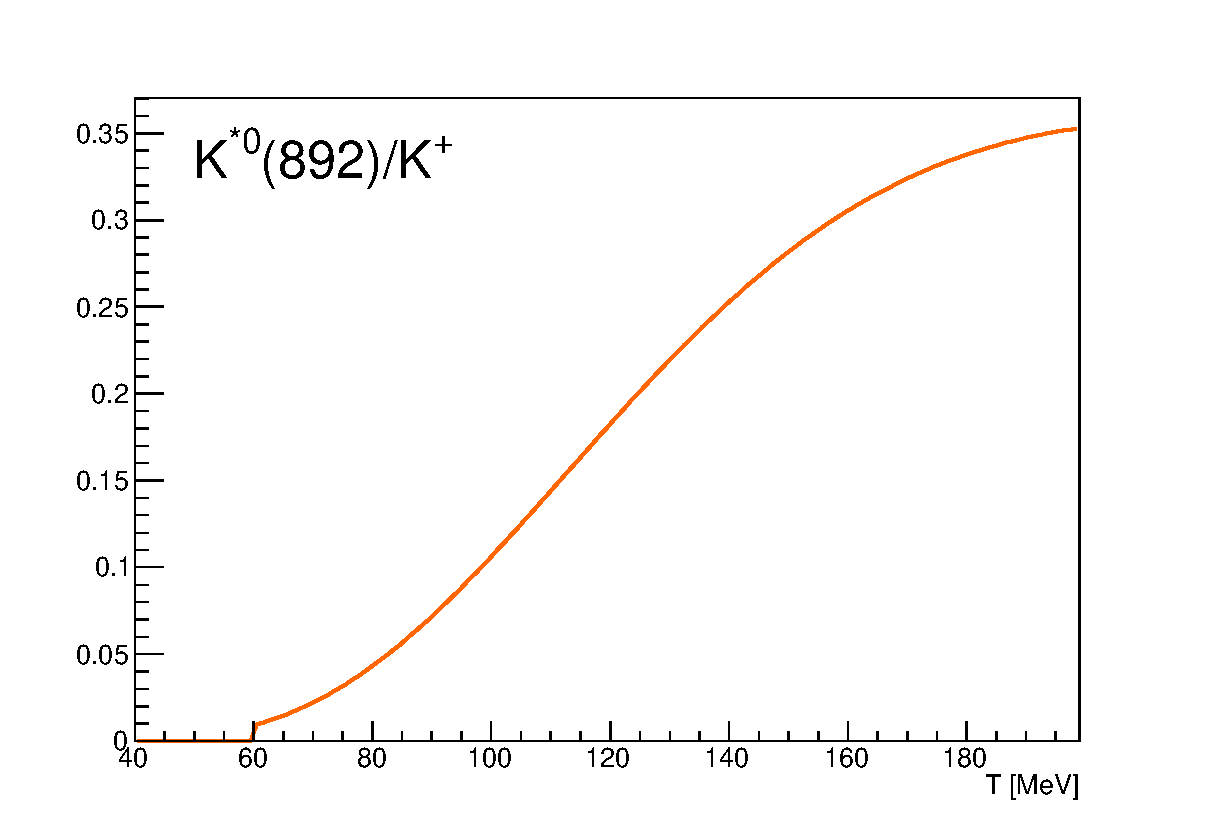
\includegraphics[width=200px]{./Version1/FigChapter2/KStarToK}
       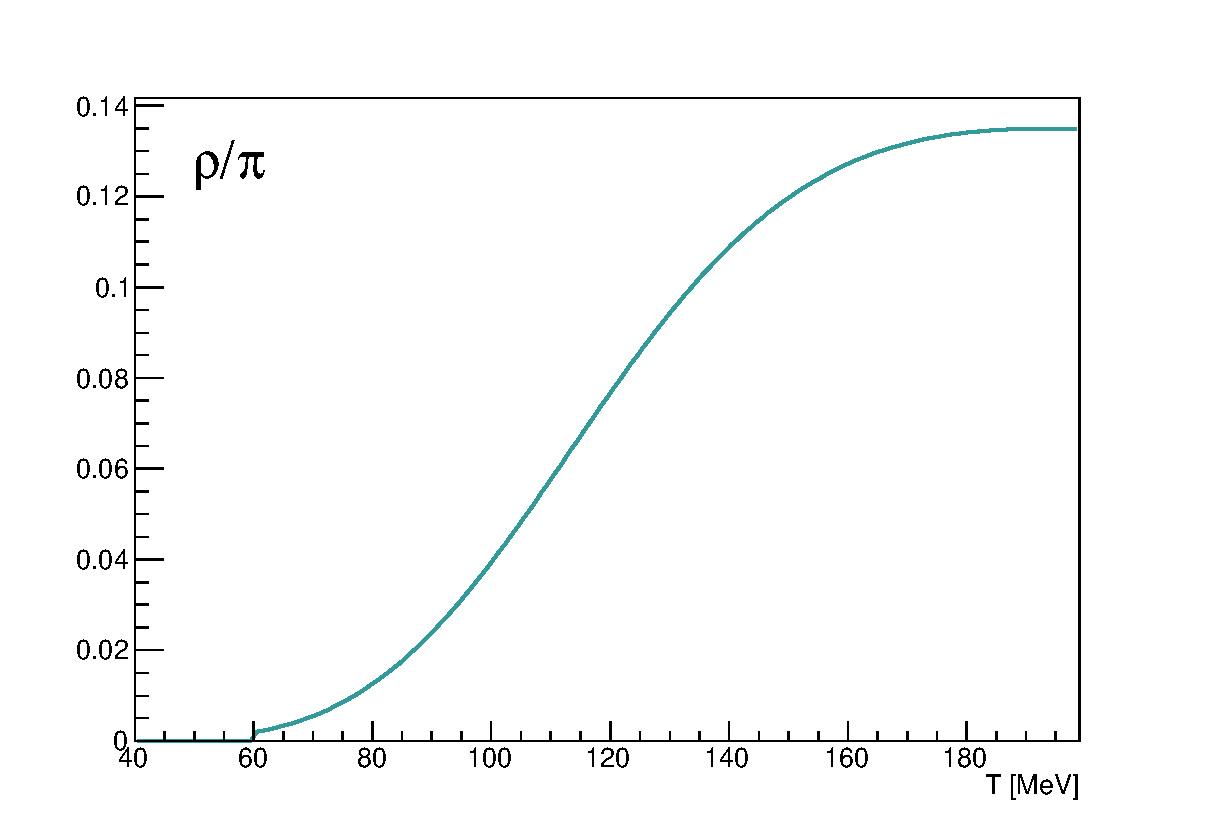
\includegraphics[width=200px]{./Version1/FigChapter2/RhoToPion}
        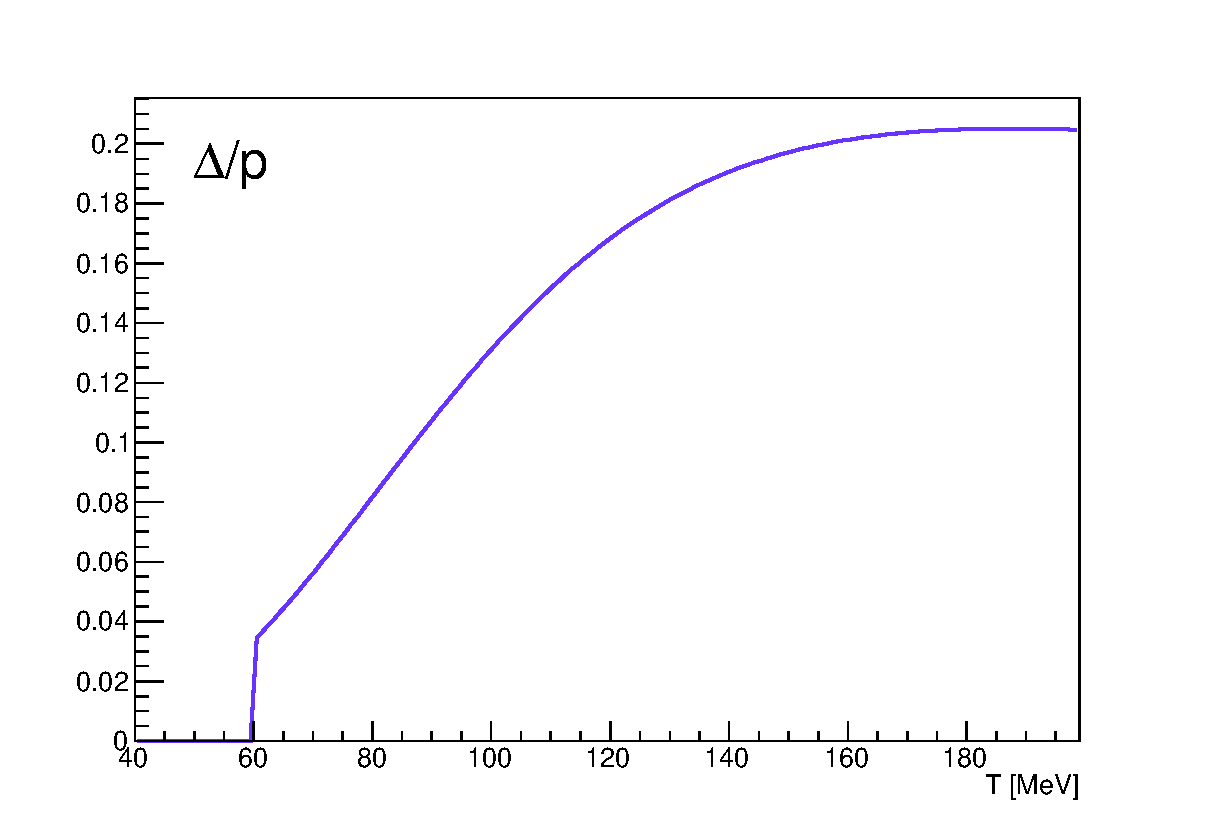
\includegraphics[width=200px]{./Version1/FigChapter2/DeltaToProton}
		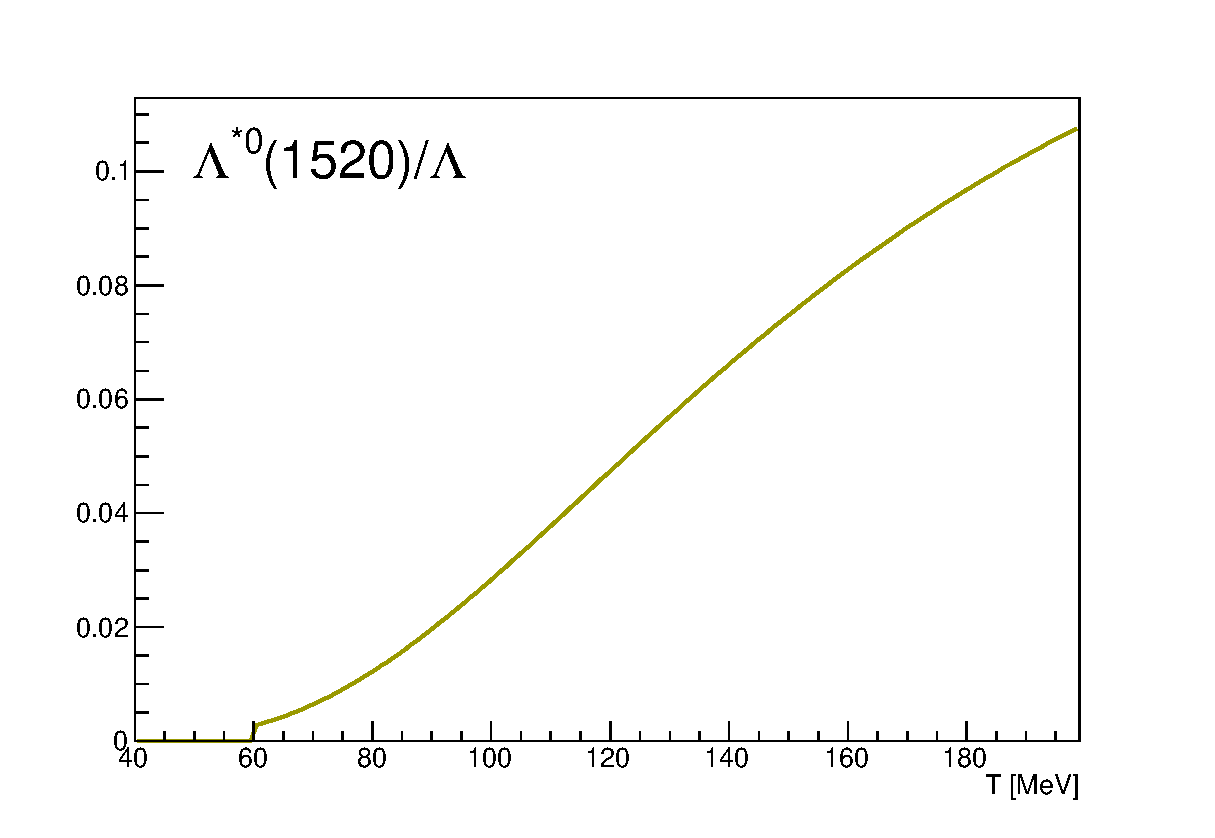
\includegraphics[width=200px]{./Version1/FigChapter2/LambdaStarToLambda}
		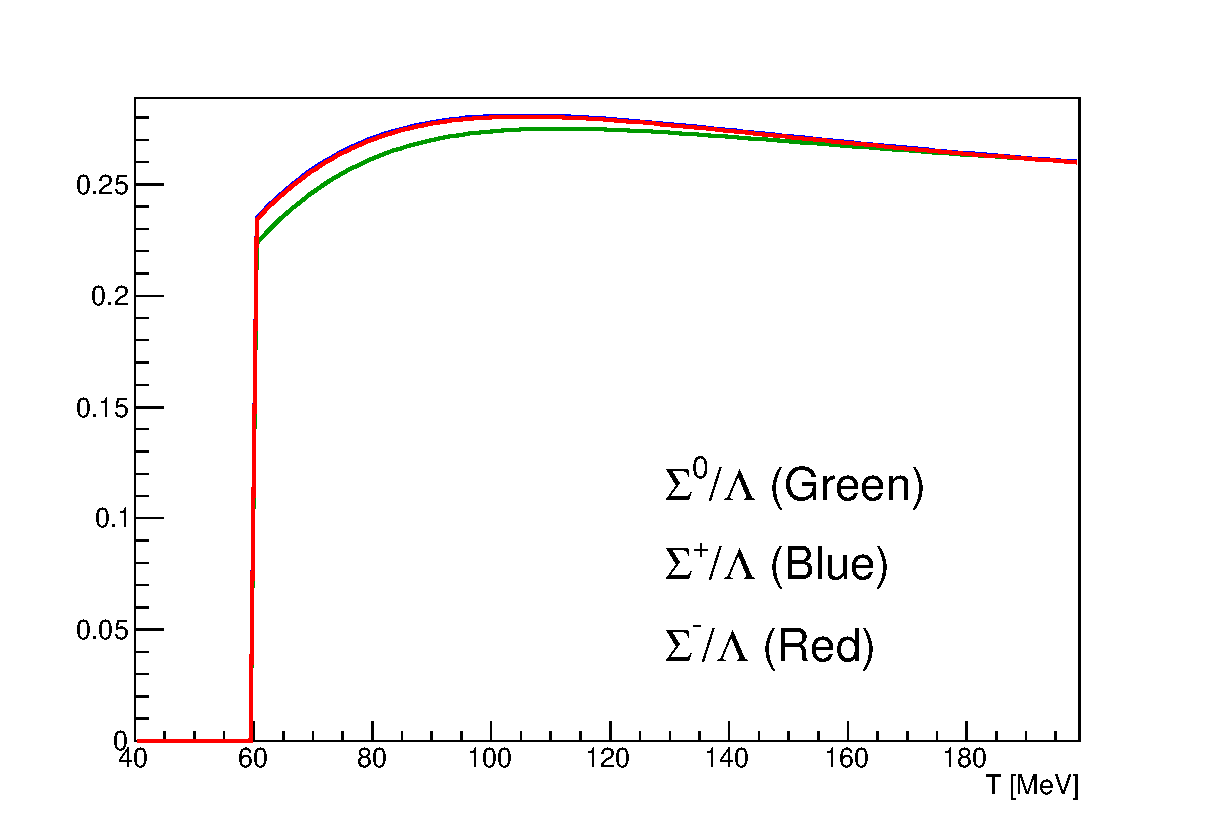
\includegraphics[width=200px]{./Version1/FigChapter2/SigmaRatio}
		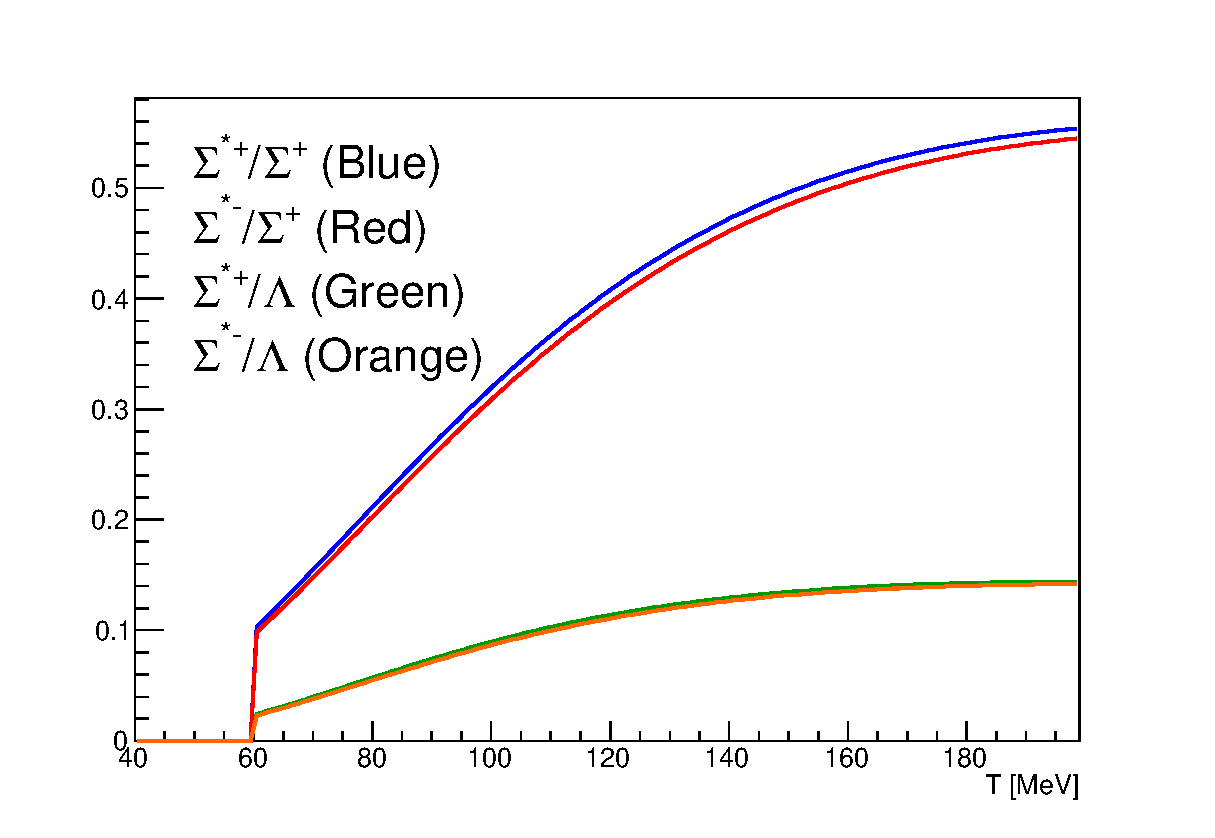
\includegraphics[width=200px]{./Version1/FigChapter2/SigmaStarRatio}
		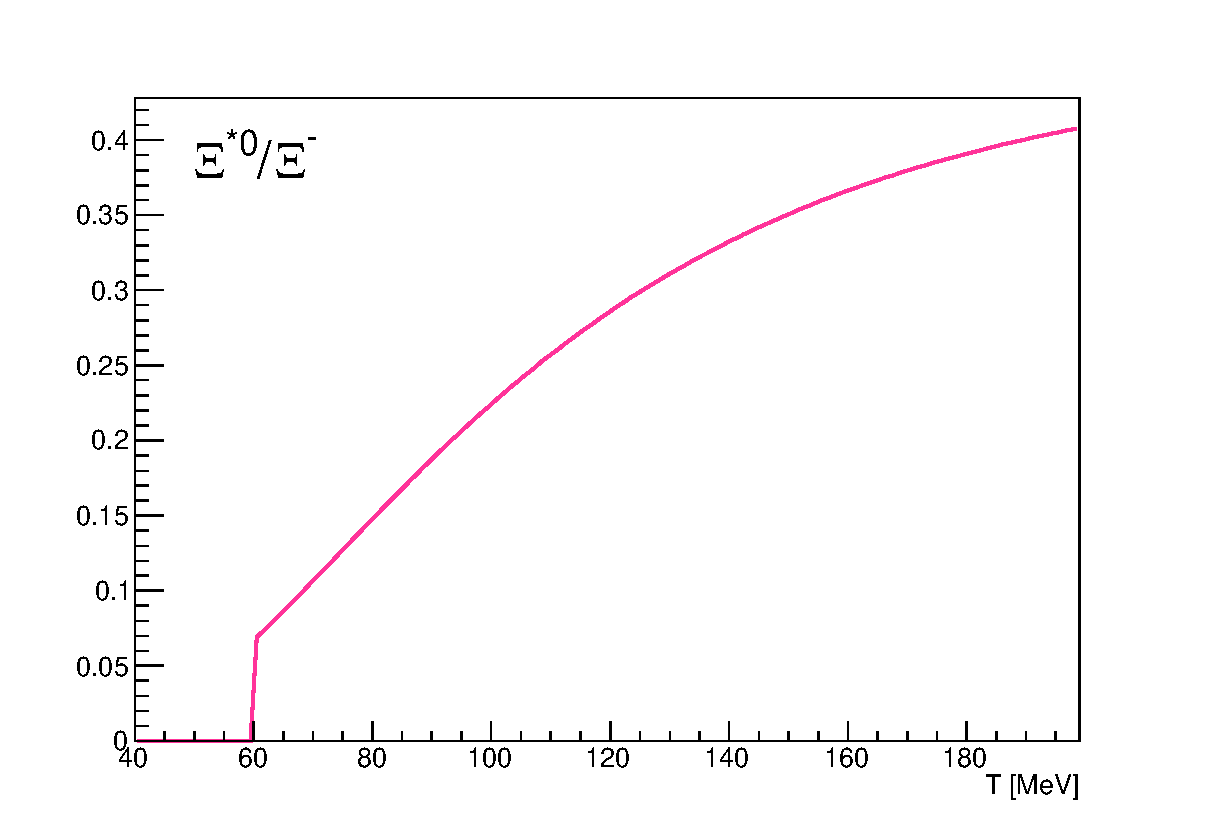
\includegraphics[width=200px]{./Version1/FigChapter2/XiStarToXi}
		\caption{\label{result1} Ratio of baryonic and mesonic resonances over their stable partner as a function of temperature.}
	\end{center}\hspace{2pc}%
\end{figure}




\begin{figure}[!htbp]
\begin{center}
	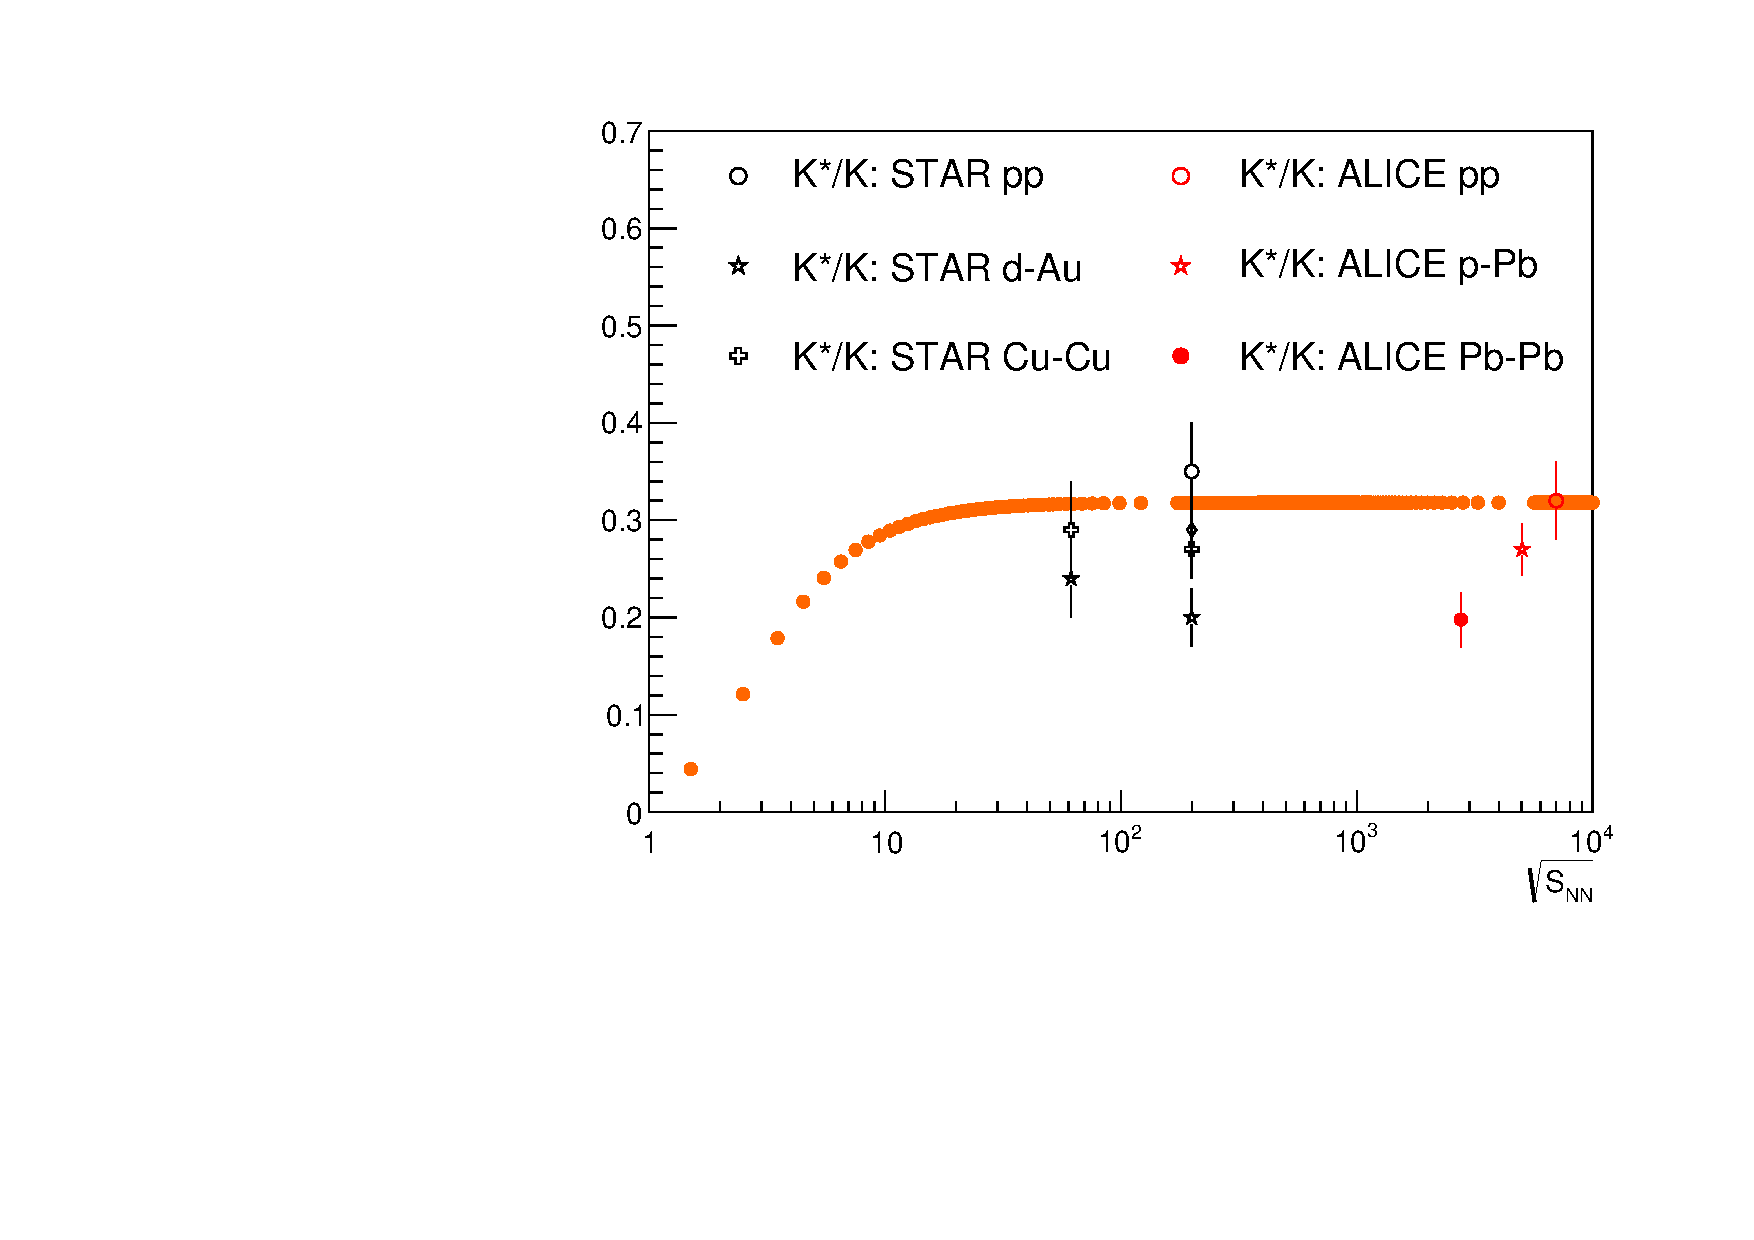
\includegraphics[width=200px]{./Version1/FigChapter2/Kstar_sqrt_s.pdf}
	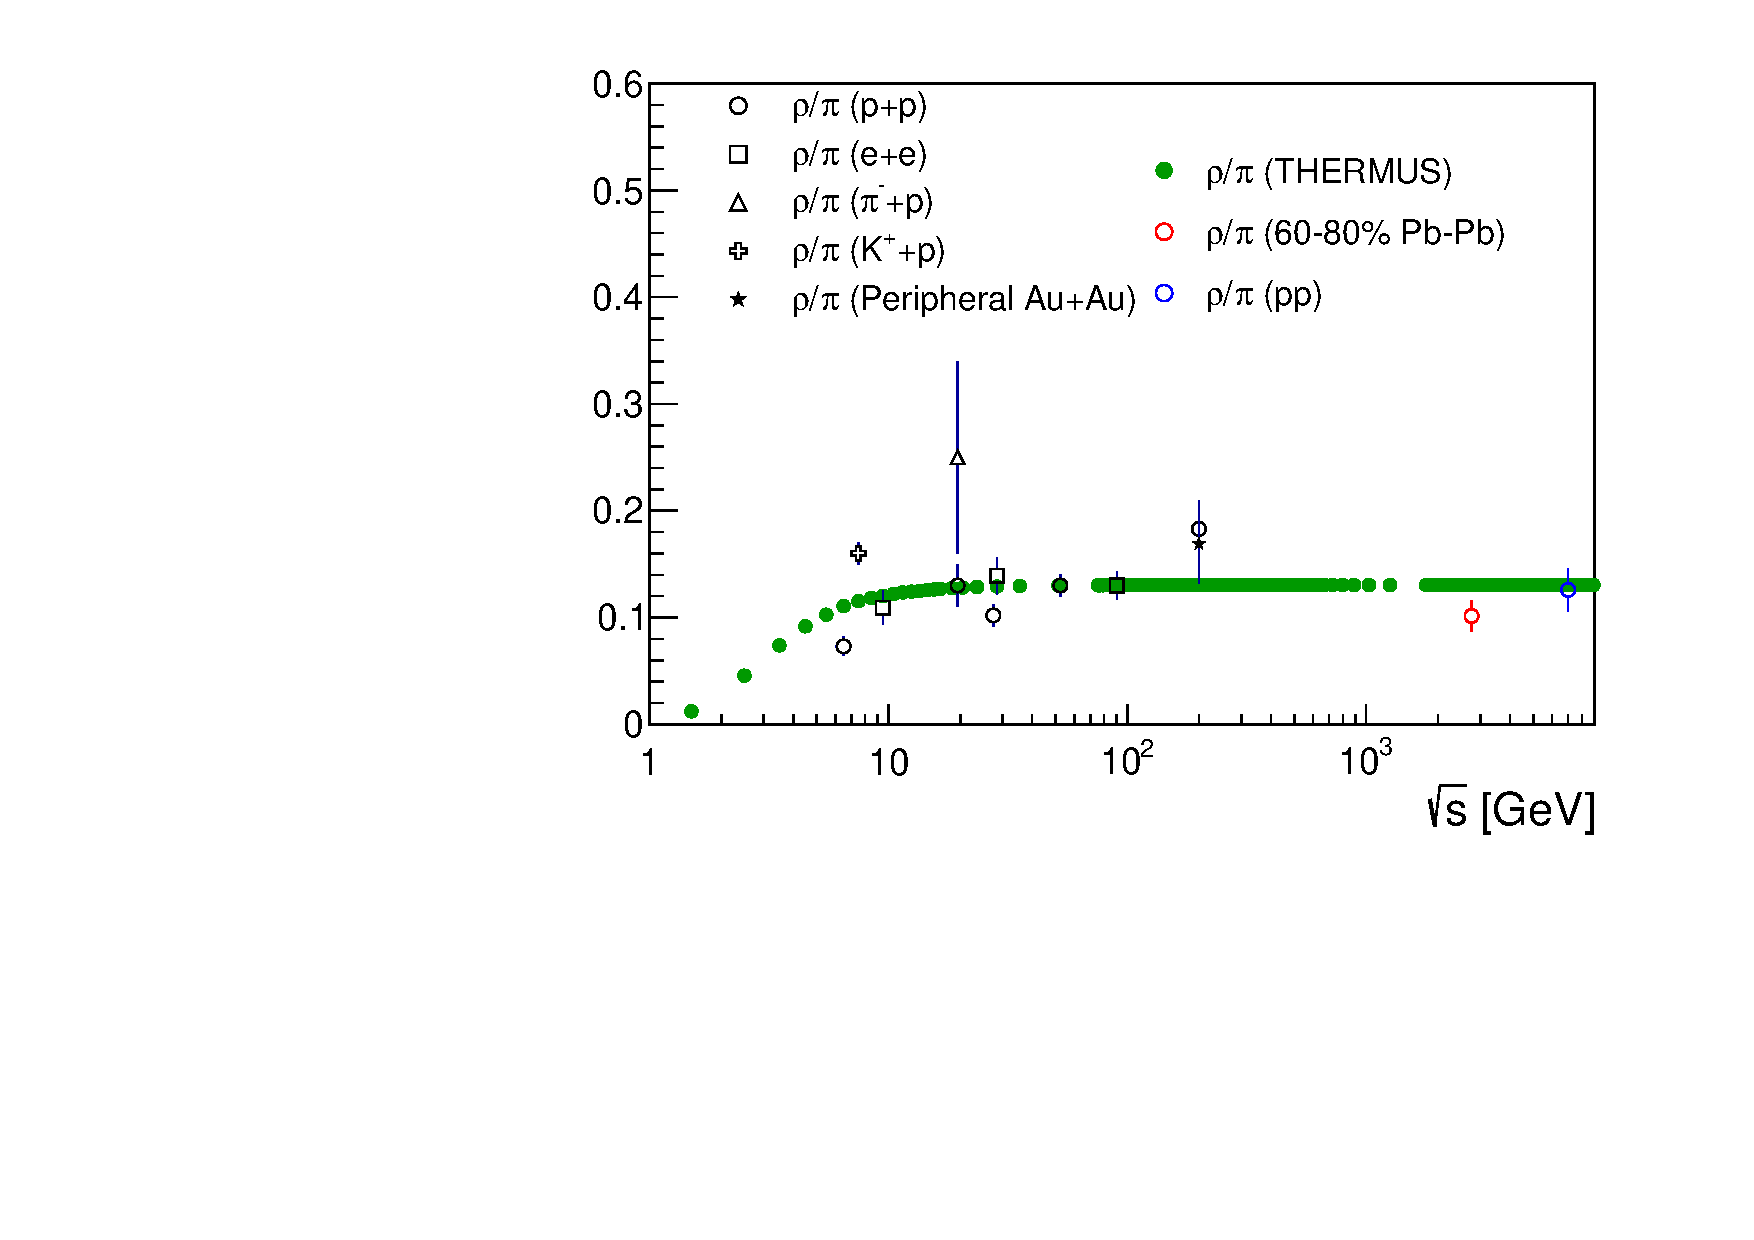
\includegraphics[width=200px]{./Version1/FigChapter2/RhoToPion_sqrt_s.pdf}
	\caption{\label{result2} Ratio of resonances over their stable partner as a function of $\sqrt{(s)}$.}
\end{center}\hspace{2pc}%
\end{figure}


\newpage

\subsection{EPOS, UrQMD}
The EPOS3 model \cite{cite:EPOSa, cite:EPOSb, cite:EPOSc} describes the full evolution of a heavy-ion collision. The initial stage is treated via a multiple-scattering approach based on Pomerons and strings. The reaction volume is divided into a core and a corona part \cite{cite:EPOSd}. The core is taken as the initial condition for the QGP evolution, for which one employ viscous hydrodynamics. The corona part is simply composed of hadrons from string decays. After hadronisation of the fluid (core part), these hadrons and as well the corona hadrons are fed into UrQMD \cite{cite:URQMDa, cite:URQMDb}, which describes hadronic interactions in a microscopic approach. The chemical and kinetic freeze-outs occur within this phase. The chemical freeze-out is expected to occur shortly after the phase transition from partonic to hadronic matter and is followed by the kinetic freeze-out.


As explained in \cite{cite:EPOSa, cite:EPOSb, cite:EPOSc, cite:EPOSd}, EPOS3 is an event generator based on 3+1D viscous hydrodynamical evolution starting from flux tube initial conditions, which are generated in the Gribov-Regge multiple scattering framework. An individual scattering is referred to as a Pomeron, identified with a parton ladder, eventually showing up as flux tubes (or strings). Each parton ladder is composed of a pQCD hard process, plus initial and final state linear parton emission. Nonlinear effects are considered by using saturation scales $Q_{s}$, depending on the energy and the number of participants connected to the Pomeron in question.


The final state partonic system (corresponding to a Pomeron) amounts to (usually two) color flux tubes, being mainly longitudinal, with transversely moving pieces carrying the \pt of the partons from hard scatterings. One has two flux tubes based on the cylindrical topology of the Pomerons. Each quark- antiquark pair in the parton ladder will cut a string into two; in this sense one may have more than two flux tubes. In any case, these flux tubes eventually constitute both bulk matter, also referred to as ?core? (which thermalizes, flows, and finally hadronizes) and jets (also referred to as ?corona?), according to some criteria based on the energy of the string segments and the local string density. For the core, we use a 3+1D viscous hydrodynamic approach, employing a realistic equation of state, compatible with lQCD results. We employ for all calculations in this paper a value of ?/s = 0.08. Whenever a hadronisation temperature of TH is reached, we apply the usual Cooper-Frye freeze-out procedure, to convert the fluid into particles. We use TH = 166MeV. From this point on, we apply the hadronic cascade UrQMD \cite{cite:URQMDa, cite:URQMDb}, about which more details are given later. All hadrons participate in the cascade, including those from the core (after freeze- out) and the corona. The corona particles, from string decay, are only ?visible? after a certain formation time (some constant of order one fm/c), multiplied by the corresponding gamma factor), so very high \pt particles have a good chance to escape.

The UrQMD model is a non-equilibrium transport approach. The interactions of hadrons in the current version include binary elastic and 2 $\rightarrow$ n inelastic scatterings, resonance creations and decays, string excitations, particle + antiparticle annihilations as well as strangeness exchange reactions. The cross sections and branching ratios for the corresponding interactions are taken from experimental measurements (where available), detailed balance relations and the additive quark model. The model describes the full phase-space evolution of all hadrons, including resonances, in a heavy- ion collision based on their hadronic interactions and their decay products. Due to the short lifetime of resonances, their decay products may interact in the hadronic phase. This is not the case for weak decays, where the system has already decoupled at the time of the decay. As discussed previously, the experimental reconstruction of resonances will be influenced by the final state interactions of the decay products. Resonance signals have been previously studied using the UrQMD model. 


\newpage
%\section{Production of resonance with strangeness}
%\subsection{Resonance with strangeness}

\section{Production of hyperon resonance}

The Quark Model, proposed independently by Murray Gell-Mann and Yuval Ne'eman in 1964 \cite{cite:gellmann}, enables the classification of hadrons in terms of their constituent quarks. In this model, the lighter mesons and baryons are representations of an SU$_{f}$(3) group, whose fundamental representation is the three dimensional vector (u, d, s). These are the three lighter quarks whose characteristics are reported in Table ref{table:quark}. 

\begin{table}[h!]
\centering
\begin{tabular}{lclclc|c|}
\hline
Light flavor &   d  & u  & s \\
\hline \noalign{\smallskip}
Baryon number (B) &  +1/3     & +1/3  &  +1/3\\
Electric charge (Q) &   -1/3     &  +2/3 &   -1/3 \\
Isospin (I)               &   -1/2     &  +1/2 &     0\\
Strangeness (S)     &     0   & 0 & -1\\
mass (\mmass)   &    2.3$_{-0.5}^{+0.7}$    & 4.8$_{-0.3}^{+0.5}$  &  95$\pm$5\\
\hline\noalign{\smallskip}
\noalign{\smallskip}
\end{tabular}
\caption{Quantum numbers and masses associated to the three lighter quarks: u, d and s}\label{table:quark}
\end{table}

The hadronic state are obtained from the decomposition of the following scalar products of the fundamental representations of the group: \\

Meson (q$\bar{q}$) :  3 $\bigotimes$ $\bar{3}$ =  1 $\bigoplus$ 8 \\

Baryon (qqq) : 3 $\bigotimes$ 3 $\bigotimes$ 3  =  10$_{S}$ $\bigoplus$ 8$_{M}$ $\bigoplus$ 8$_{M}$ $\bigoplus$ 1$_{A}$ \\

For the baryons without $c$ or $b$ qaurk, flavor and spin may be combined in an approximate flavor-spin SU(6), in which the six basic states are d $\uparrow$, d $\downarrow$, $\cdot$ $\cdot$ $\cdot$, s $\downarrow$ ($\uparrow$, $\downarrow$ = spin up, down). Then the baryons belong to the multiplets on the right side of \\

6 $\bigotimes$ 6 $\bigotimes$ 6  =  56$_{S}$ $\bigoplus$ 70$_{M}$ $\bigoplus$ 70$_{M}$ $\bigoplus$ 20$_{A}$ \\

Here, the 56 representation can be decompose in an octet ($J^{P}$ = 1/2$^{+}$) and a decuplet ($J^{P}$ = 3/2$^{+}$), as can be seen in Figure \ref{fig:octet} and Figure \ref{fig:decuplet}.

\begin{figure}[htbp]
\begin{center}
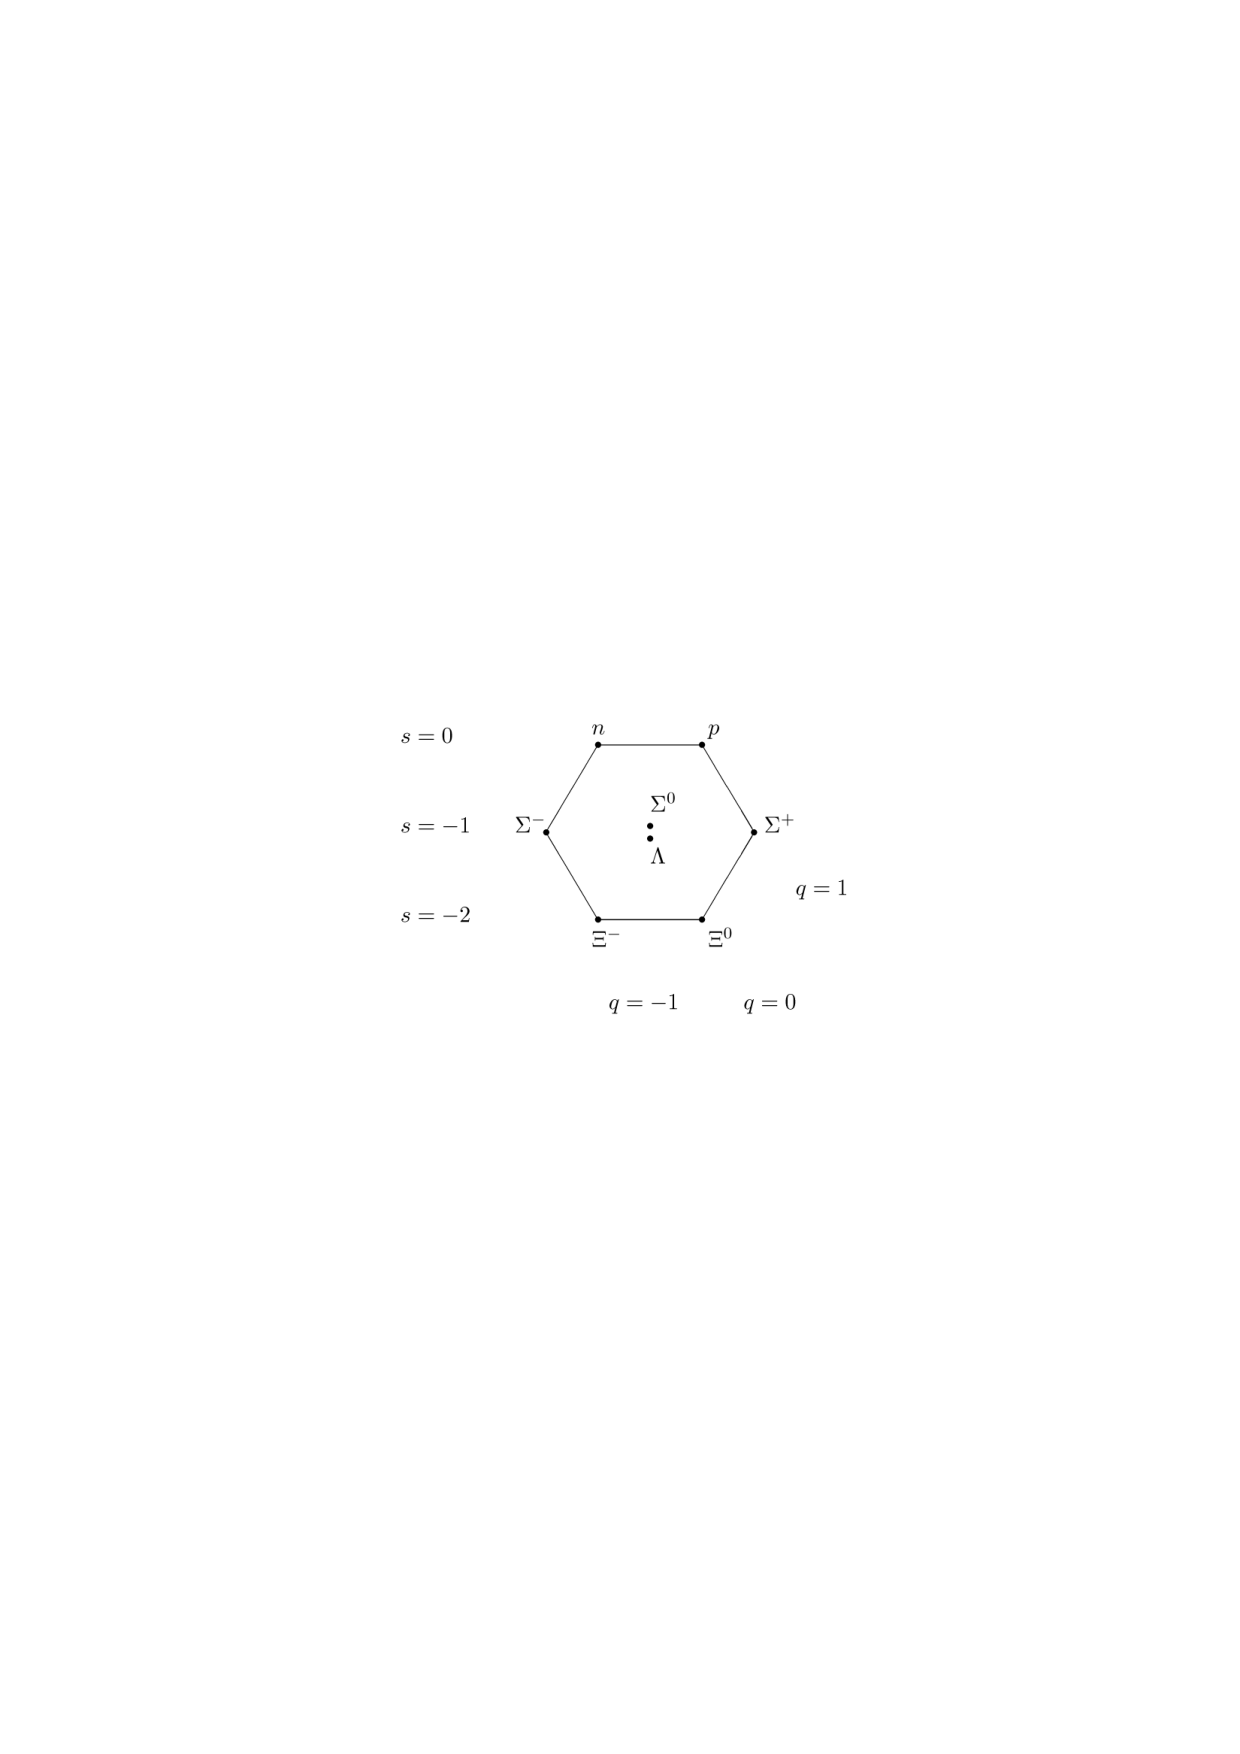
\includegraphics[width=10.cm]{./Version1/FigChapter3/Octet}
\caption{ The $J^{P}$ = 1/2$^{+}$ ground state baryon octet}
\label{fig:octet}
\end{center}
\end{figure}

\begin{figure}[htbp]
\begin{center}
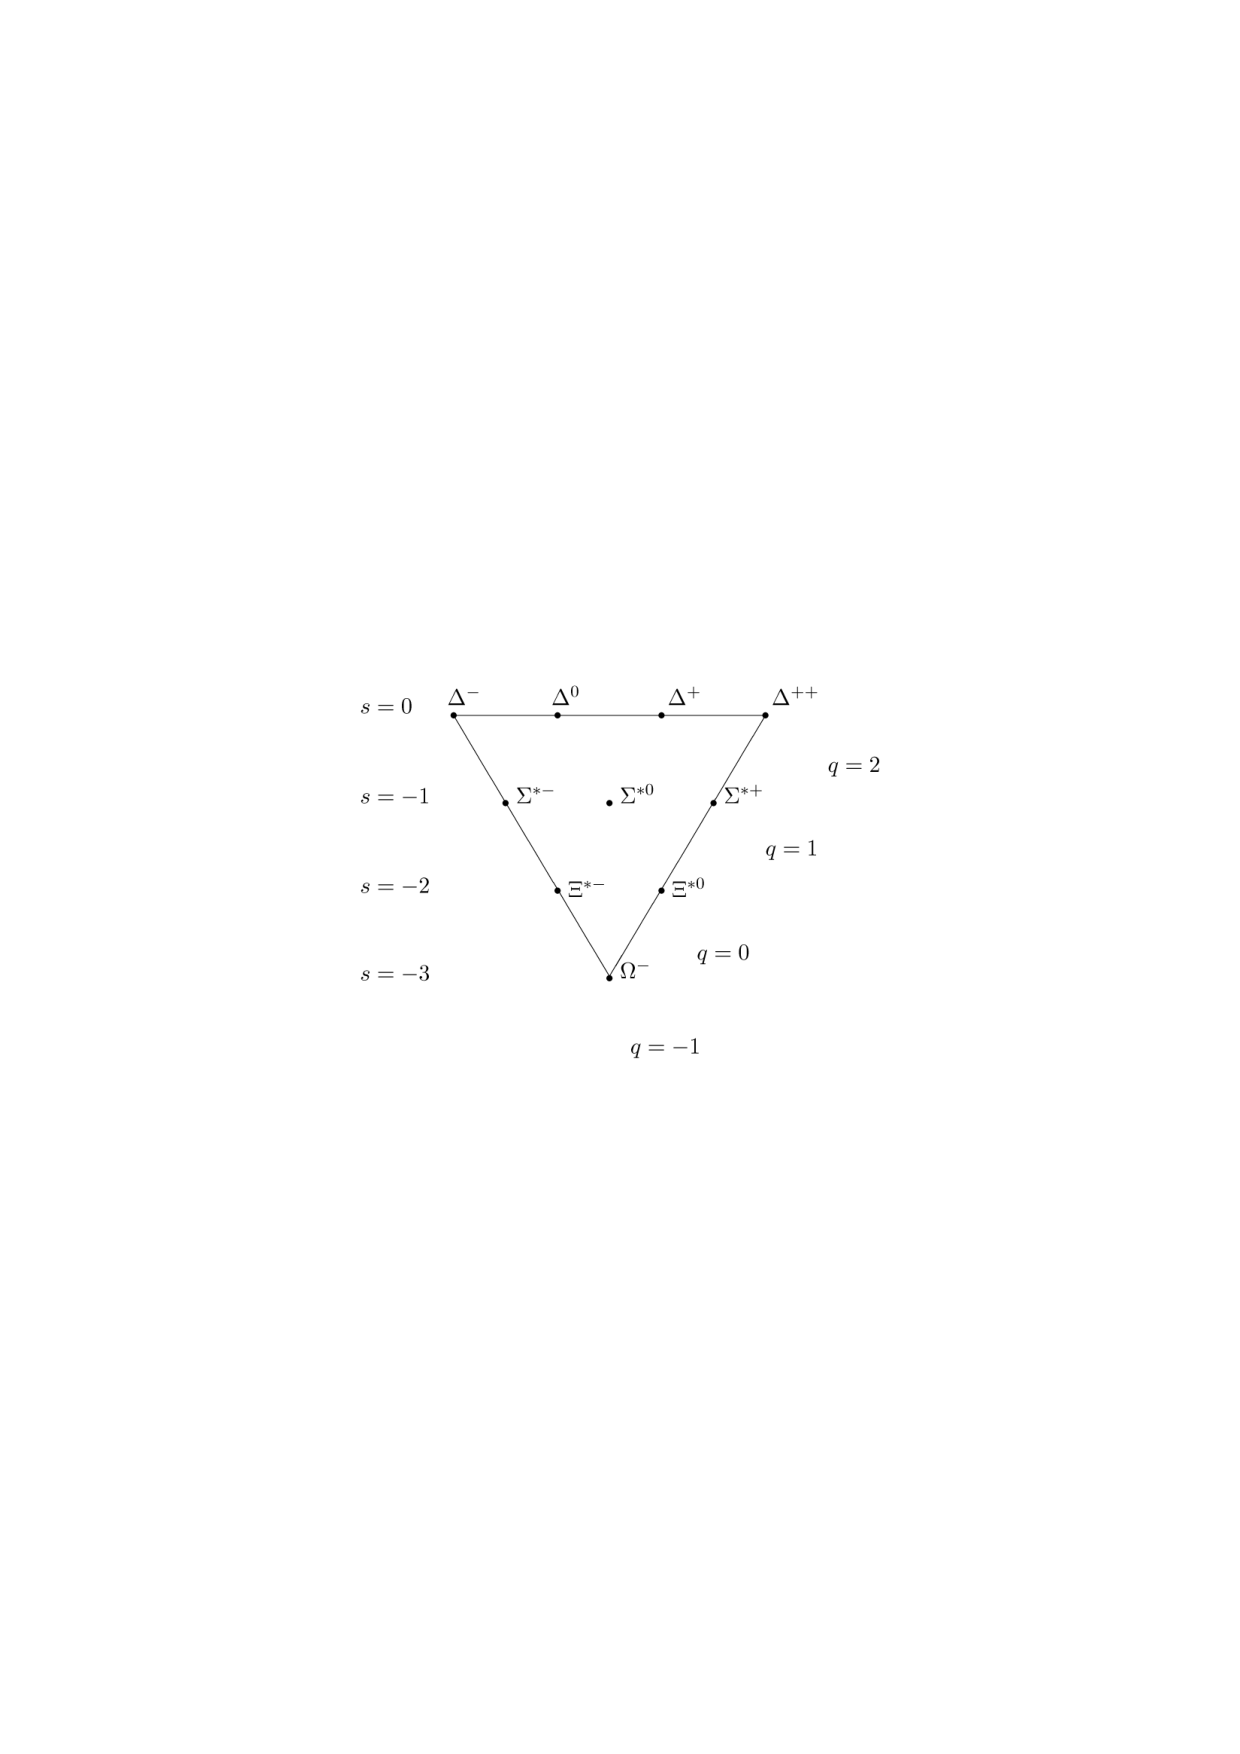
\includegraphics[width=10.cm]{./Version1/FigChapter3/Decuplet}
\caption{ The $J^{P}$ = 3/2$^{+}$ baryon decuplet}
\label{fig:decuplet}
\end{center}
\end{figure}

Among these hadrons, the special family of particles that contain at least one strange quark but not heavier quarks (like charm or bottom), are called hyperons. These are: the $\Lambda$(uds), the triplet $\Sigma^{+}$(uus), $\Sigma^{0}$(uds), $\Sigma^{-}$(dds), the doublet $\Xi^{-}$(dss), $\Xi^{0}$(uss) and the $\Omega$(sss) and the corresponding antiparticles. $\Xi$ and $\Omega$ are the only hyperons containing more than one strange quark, hence they are called multi-strange baryons. 
Resonances shown in Figure ref{fig:decuplet} having * with its name (e.g. X*$^{\pm}$) are particles which have higher mass than the corresponding ground state particle with the same quark content. 

Different resonances having various lifetimes (Table \ref{table:rsnptl}) can be used as tool to explore different stages of the fireball expansion as discussed in section \ref{sec:hi}. In order to have insight on the role of the re-scattering effect between the freeze-out phases, it is important to measure the ratio between resonances and stable hadrons and  compare it with different lifetimes. 


\begin{table}[h!]
%\centering
\begin{center}

\begin{tabular}{|c|c|c|c|c|c|c|clc|c|c|}
\hline
Particle & $\rho$(770) & $\Delta$(1232) &K*(892) & $\Sigma$(1385) &$\Lambda$(1520) & $\Xi$(1530)& $\Phi$(1020)\\
\hline
Lifetime[c$\tau$] &  1.3 fm &1.7 fm & 4.0 fm& 5.5 fm& 10.3 fm & 22 fm& 46 fm\\
\hline
\end{tabular}
\caption{Lifetime of hadronic resonances}\label{table:rsnptl}
\end{center}
\end{table}



In the following, a general overview of the role of the strange quark within the QGP studies with heavy-ion collisions is given.
%First of all, no net strangeness is present in the colliding objects before collision. Indeed, both the nucleons, proton and neutron, contain only u and d quarks among their valence quarks. All the net strangeness present in the final states (particles) is then created during the collision, and therefore the s quark plays an interesting role in the study of particle production.
And importance of the measurement of resonance is explained as probe of properties in the duration of hadronic phase from the chemical($T_{ch}$) to the kinetic freeze-out($T_{kin}$). 



\subsection{Strange quark and hyperons}
  
The original interest in the strangeness in the context of the QGP comes from an idea by Johann Rafelski and Berndt M$\ddot{u}$ller. In 1982, they suggested a possible signature for the formation of a QGP in a heavy-ion collision \cite{cite:strangeness}. The key argument, at a fixed collision energy, rests on the different production mechanism of the s quark within two different systems:
\begin{description}
\item[1. Hadron Gas (HG)], where the degrees of freedom are the hadronic ones, as quark and gluons are confined.
The great abundance of pions in the HG suggests to consider the production of strange particles from the reaction between them.
Direct production can be observed with $\pi$ + $\pi$ $\rightarrow$ $\pi$ + $\pi$ + strange hadron + antiparticle, considering the baryon and strange number conservation. This means that, in order to create the strange particle and anti-particle at once, the reaction threshold (energy needed to produce mesons or baryons) corresponds to tow times the rest mass of the hadrons. (2230 MeV for $\Lambda$+$\bar{\Lambda}$, 2642 MeV for $\Xi$+$\bar{\Xi}$. 3344 MeV for $\Omega$+$\bar{\Omega}$)

%In the case of indirect production, the thresholds are lower. In this case, one would have two reactions in a sequence, starting with the production of lighter hadrons (? + N ? K + ?) and followed by a re- action of these intermediate products to produce the heavier hadrons (?+? ? K+? and ?+? ? K+?). In this case the combined thresh- olds for the production of a ? is (535 + 565) MeV = 1100 MeV and for the production of an ? is (535 + 565 + 710) MeV = 1810 MeV.

\item[2. QGP], where the degrees of freedom are partonic ones, with quarks and gluons free with respect to each other. The high gluon density gives the possibility to have new production mechanisms abreast the usual quark-pair annihilation which are the gluon fusion processes. It becomes the dominant process of $s\bar{s}$ pairs creation. In these reactions the energy threshold is equal to the naked mass of the two strange quarks $\approx$ 2 $\cdot$ 100 MeV.
\end{description}


%The mass of the hadrons is only partly due to the mass of the constituent valence quarks.

The quarks can not be seen directly due to the strong interaction which keeps them confined. Once they are free, as in a QGP, the quarks recover their bare masses. (Note that, only the part of mass of hadron comes from the mass of the constituent quarks.)
It was predicted that, if the QGP is formed, an enhancement of the strange quarks should occur, because the production of $s\bar{s}$ pairs becomes easier due to the lower energy needed as explained above. When the QGP cools down, these strange quarks eventually recombine into hadrons favoring also an enhancement of the number of strange hadrons. This effect is larger for hadrons with higher strangeness, with the following scaling for the number type: \\
Ordering in QGP: $N_{\Omega} >  N_{\Xi} > N_{\Lambda}$

where $N_{\Omega}$, $N_{\Xi}$, $N_{\Lambda}$ are the number of produced $\Omega$, $\Xi$ and $\Lambda$. A certain enhancement of strange hadrons can occur also in a hadron gas system, but the processes of hadronisation in this case are relatively easy for K and  $\Lambda$. and progressively harder for hadrons with higher strangeness, hence the relation would be: \\
Ordering in HG: $N_{\Omega} <  N_{\Xi} < N_{\Lambda}$.

The measurement of multi-strange hadrons in heavy-ion collisions with respect to small collisions is considered to be a signature of the formation of the QGP and it was observed at SPS, RHIC and LHC. \cite{cite:strangePbPb}


\begin{figure}[htbp]
\begin{center}
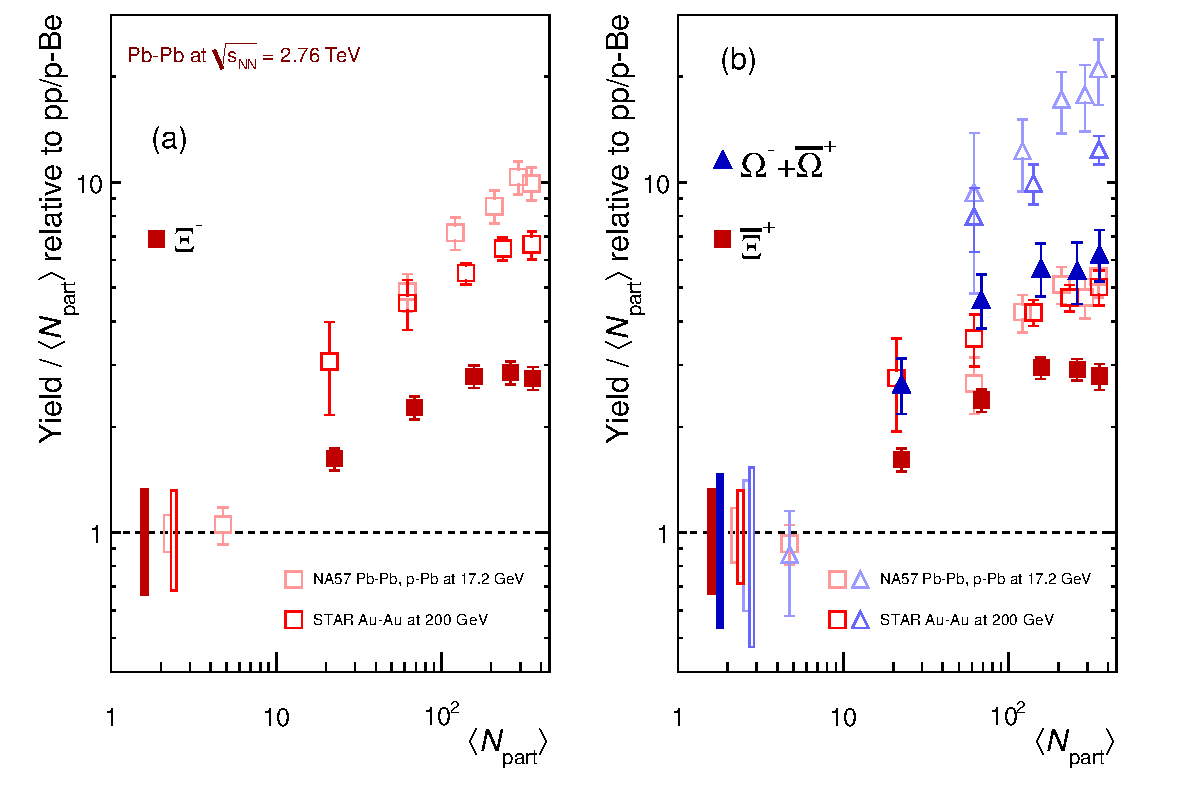
\includegraphics[width=12.cm]{./Version1/FigChapter3/MultdNdy}
\caption{Integrated yield relative to small system (pp or p--Be) as a function of the mean number of participants  $\langle N_{part}\rangle$ in the rapidity range $\arrowvert y \arrowvert<$0.5. The results from ALICE are presented as full symbols, RHIC and SPS data are shown as open symbols. Boxes on the dashed line at unity represent statistical and systematic uncertainties on the pp or p-Be reference.}
\label{fig:dNdy}
\end{center}
\end{figure}


The measured enhancement factors of baryons with increasing strangeness content are reported in Figure \ref{fig:dNdy} as a function of the mean number of participants, $\langle N_{part}\rangle$, compared with measurements at SPS and RHIC. 
As shown in the Figure \ref{fig:dNdy}, the enhancement increases with $\langle N_{part}\rangle$ which is variable to be comparable to the centrality in Pb--Pb collisions and the effect is more pronounced for particle with larger strangeness content. If one consider the collision energy dependency, the comparison with measurement from the previous experiment shows that the relative enhancements degrease with increasing energy.  An explanation of this behavior is given in terms of a statistical model, with canonical strangeness conservation. 

In a large system with a large number of produced particles, the conservation law of a quantum number, e.g., strangeness, can be implemented on the average by using the corresponding chemical potential. This is the Grand Canonical formulation that was discussed in previous Section. In a small system, however, with small particles multiplicities, conservation laws must be implemented locally on an event-by-event basis. 

This is the Canonical formulation which conservation of quantum numbers is known to severely reduce the phase space available for particle production.\cite{cite:suppression}. This canonical suppression factor decreases with lower energy in the centre of mass of the collisions and could explain the larger enhancement for lower energy systems.



\subsection{Resonance production}

\begin{figure}[htbp]
\begin{center}
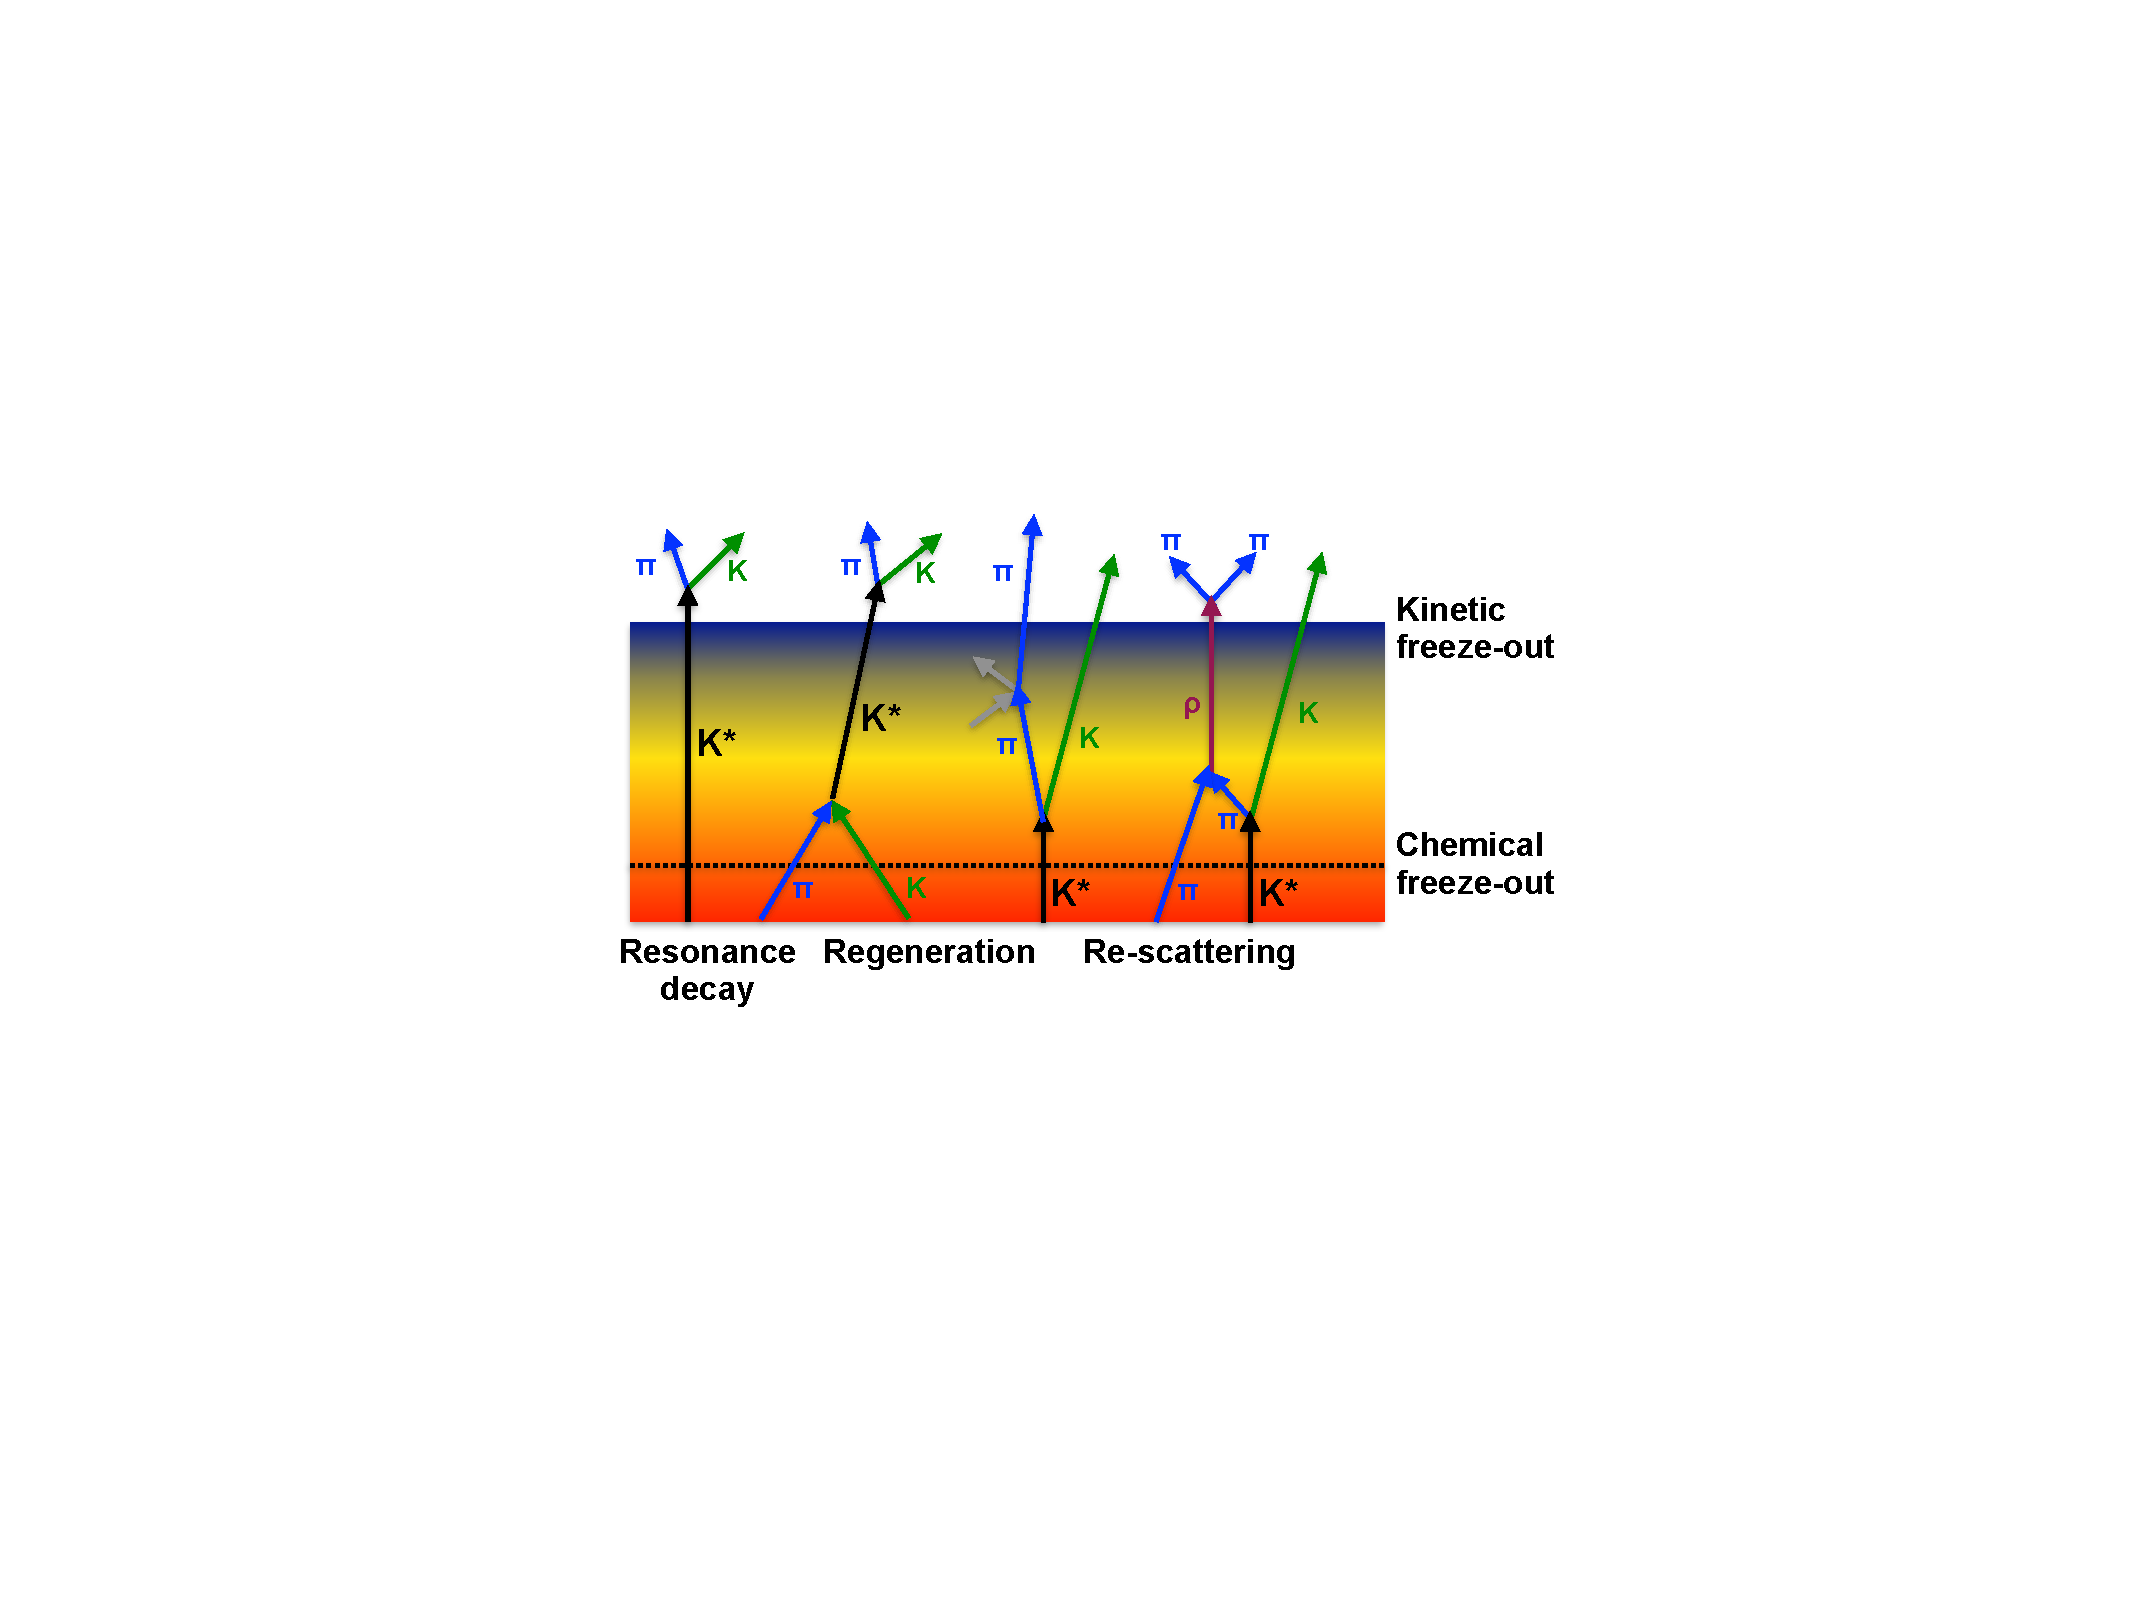
\includegraphics[width=12.cm]{./Version1/FigChapter3/Hadronic}
\caption{Hadronic phase }
\label{fig:hadronic}
\end{center}
\end{figure}



Resonances are particles with larger mass than the corresponding its ground state particle which has the same quark content. Because of the hadronic resonances decay strongly in the medium, it has short lifetime($\tau$) in the order of few fm/c which is comparable to the lifetime of the fireball. The natural width of resonances is given by $\Gamma = \bar{h}$/$\tau$, which is inversely proportion to the lifetime. 
In heavy-ion collisions, the hadronic resonances are produced in medium which is still expanding so that the particles could interact with the medium and decay while traveling it. The particles can be measured only via reconstruction of their decay products in a detector, since it decays very shortly after being produced.

The effects which can be happened in the hadronic phase is shown in Figure \ref{fig:hadronic}. In the left on the figure, as example, there is sketch of the original resonance decay of K*(892)$^{0}$ (K*(892)$^{0}$ $\rightarrow$ $\pi$+K). It is possible that resonances may be regenerated via pseudo-elastic scattering of decay products ( $\pi$+K $\rightarrow $ K*(892)$^{0}$ $\rightarrow$ $\pi$+K) in the time duration between the chemical ($T_{ch}$) and the kinetic freeze-out ($T_{kin}$).
Conversely, in case that the decay product undergo elastic scattering or pseudo-elastic scattering through a different resonance in the medium, e.g. $\rho$ in the Figure \ref{fig:hadronic}, the invariant mass of the daughters can not mach that of the parent particle. As a results, yield after kinetic freeze out could be smaller than the yields originally produced.

These re-scattering and regeneration depend on the lifetime of the resonances and affect the their yield and momentum spectrum. The yield is increase if the regeneration dominates, vice versa, it is decrease with re-scattering effect. In order to understand the properties in hadronic medium, the ratios between resonances and stable hadrons have to be studies and the results are compared with model predictions discussed in Section \ref{sec:model}.




\newpage
%\section{Theoretical models}
%\subsection{Thermal statistical model}
%\subsection{UrQMD}

\newpage
\section{A Large Ion Collider Experiment at the LHC}

ALICE (A Large Ion Collider Experiment) is one of major experiment at LHC (Large Hadron Collider) in Geneva and it is dedicated experiment for the study of QCD matter created in high-energy collisions \cite{cite:ALICEPerformance}. It has been accumulating data during the whole first phase of the LHC operation, from end of 2009 to the beginning of the technical shutdown 2013. During that time, the beam energy was tuned to have data in pp collisions at 0.9, 2.76, 7 and 8 TeV, p--Pb collisions at 5.02 TeV and Pb--Pb collisions at 2.76 TeV.

The section \ref{label:lhc} aims to explain the LHC operation of the first phase and includes each experiments builed in LHC. Next section (\ref{label:alice}) focuses on general description of the ALICE detector and detailed explanation of sub-detectors used in this analysis will given. And then the particle identification performance is discussed. The Data Acquisition (DAQ) system and trigger system follow in Section \ref{label:aliceDAQ}. The last section account for offline software frame work.


\subsection{The Large Hadron Collider}\label{label:lhc}
The Large Hadron Collider (LHC) \cite{cite:LHC} at CERN is the world's largest particle accelerator. It provides maximum possible energies of 7 TeV for proton beam and 2.76 per nucleon for beam of lead ions, hence, providing collisions at \s = 14 TeV and \snn = 5.5 TeV, respectively. These energies are largest one ever achieved in particle collision experiment. 

The LHC is a two ring superconducting hadron accelerator and collider built in the 26.7 kM tunnel. 
In separate parallel beam pipe, there are two counter-rotating beams and the bunches of particles in each of them rotate many time up to collision energy is reached. The accelerator keeps to bend the beam around the ring to maintain focused bunches and enlarge them to their collision energy.
In the end, the spatial dimension of the each bunches turns into minimized to obtain high luminosity guarantee a high number of collisions per time interval at the collisions points. 
In order to acheive it, combination of magnetic and electric field have been performed. In spite of the high luminosity, very small portion of the particles of two bunches collides in a single bunch crossing. The others are defocused and continue to rotate the ring.
   
\begin{figure}[htbp]
\begin{center}
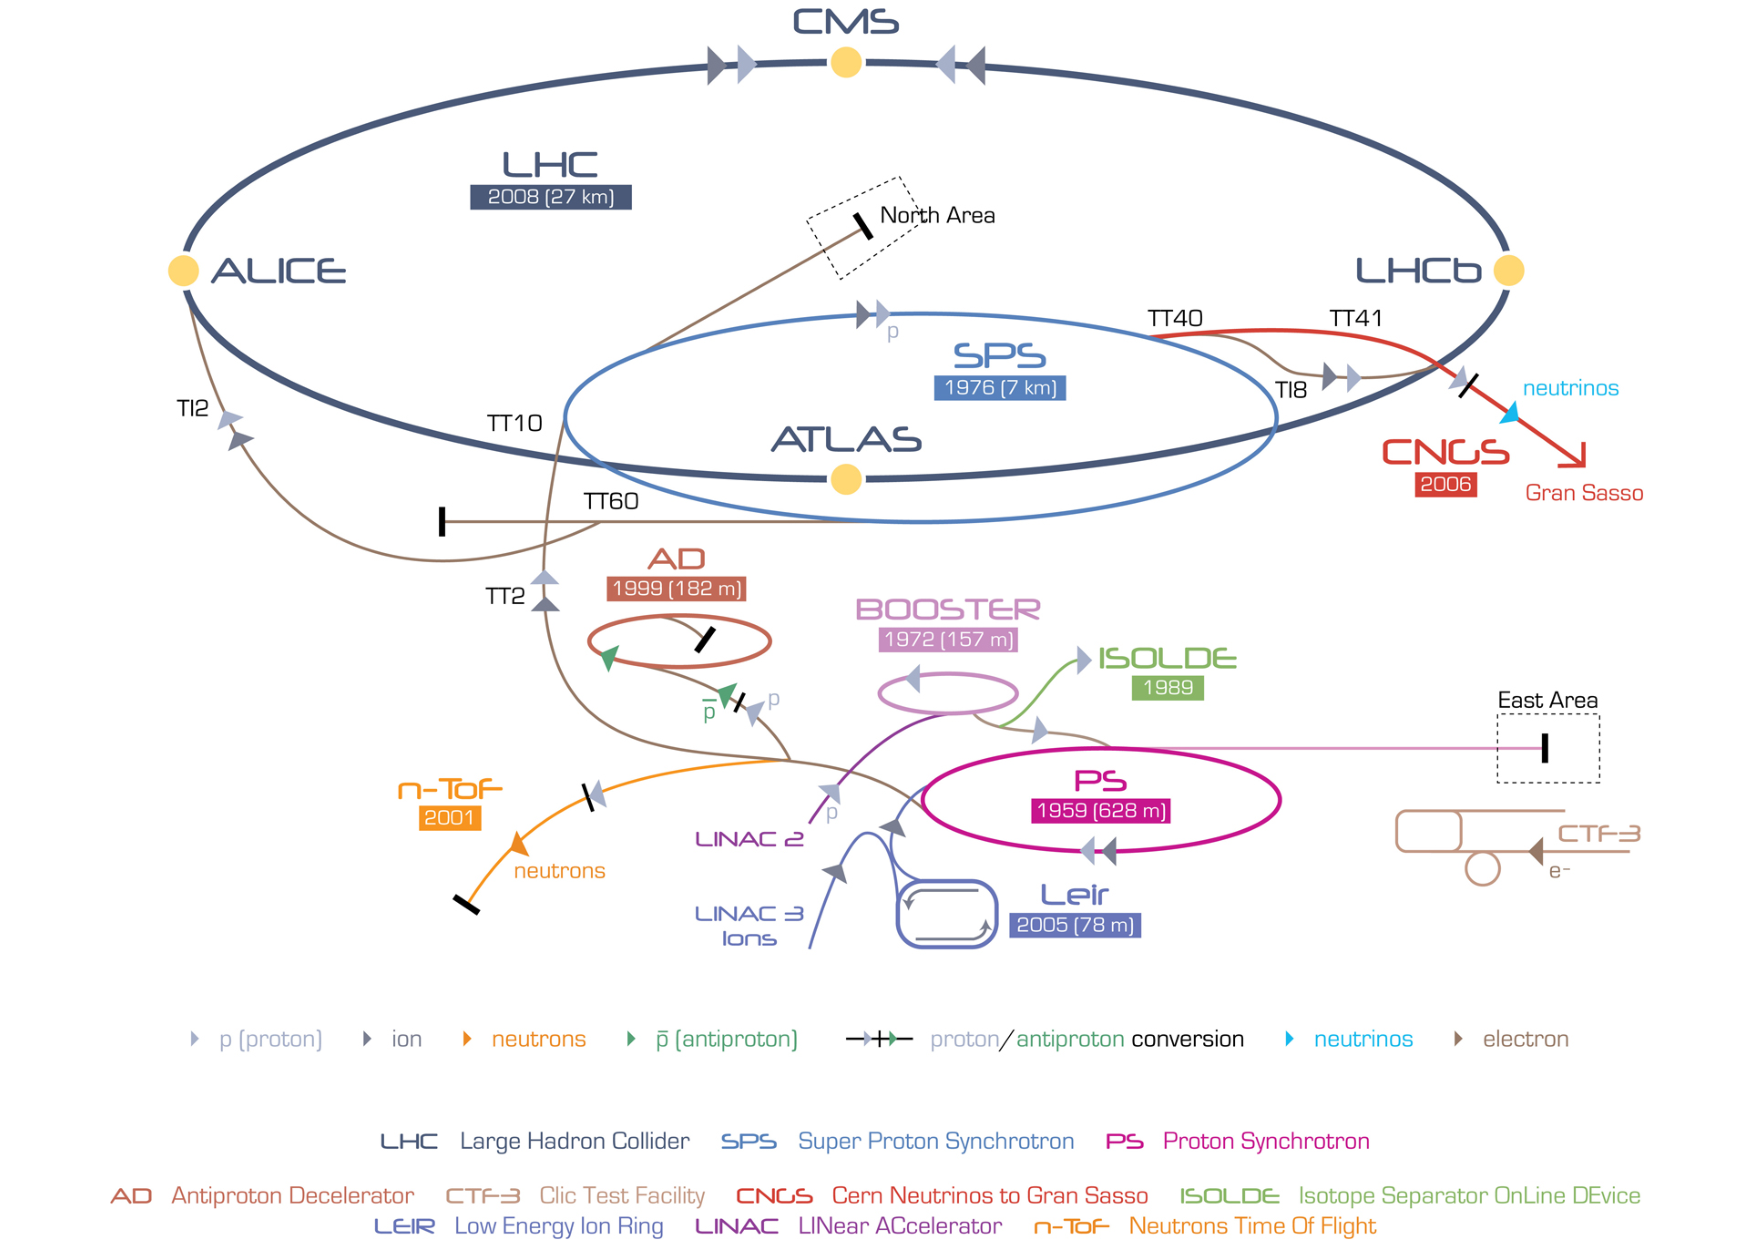
\includegraphics[width=12.cm]{./Version1/FigChapter4/FigureLHC}
\caption{ The CERN accelerator complex \cite{cite:LHCfig}}
\label{fig:lhc}
\end{center}
\end{figure}

The CERN accelerator complex is shown in the Figure \ref{fig:lhc}. The sequence of injection of bunches into the LHC is started from acceleration in the LINAC (LINear ACcelerator )2, PS (Proton Synchrotron) booster, PS, and SPS (Super Proton Synchrotron) accelerators. The way to inject of heavy-ion bunches are different. The bunches pass the LINAC3 instead of LINAC2, LEIR (Low Energy Ion Ring), PS and SPS accelerators \cite{cite:LHCinfo}. 


The first pp collisions at 900 GeV center of mass energy were delivered by the LHC on September 10th 2008. Nine days later, the operations were interrupted due to a failure in an electrical connection between two magnets. The machine operators spent over a year repairing and consolidating the accelerator. On November, 2009 low energy proton beams circulated again, and a few days later, by achieving the energy of 1.18 TeV per proton beam, LHC became the most powerful accelerator in the world. The first pp collisions at center of mass energy of 7 TeV were delivered in March 2010, and the first Pb--Pb collisions at center of mass energy of 2.76 TeV per nucleon pair in November 2010. 

In 2010 the integrated luminosity delivered by the LHC was $\sim$ 48 $pb^{-1}$ for pp collisions at \s = 7 TeV ($\sim$ 0.5 $pb^{-1}$ in ALICE) and $\sim$ 10 $\mu b^{-1}$ for Pb--Pb at \snn = 2.76 TeV ($\sim$ 9 $\mu b^{-1}$ in ALICE) \cite{cite:ALICEPerformance}. In 2011 the beam energy was the same as in 2010 both for pp and Pb--Pb. The performance of the LHC improved in terms of luminosity with $\sim$ 5.61 $fb^{-1}$ for pp ($\sim$ 4.9 $pb^{-1}$ in ALICE) and $\sim$ 166 $\mu b^{-1}$ for Pb--Pb collisions ($\sim$ 146 $\mu b^{-1}$ in ALICE). In 2012, the centre-of-mass energy for pp collisions was brought to 8 TeV and the integrated luminosity (up to December 2012, end of the pp program) was $\sim$ 23.3 $fb^{-1}$ ($\sim$ 10 $pb^{-1}$ in ALICE). A pilot p--Pb run operated at \snn = 5.02 TeV on September 2012, followed by a long p--Pb run on February 2013 with a delivered luminosity of 14 $nb^{-1}$. A very short pp run at \s = 2.76 TeV ended the Run1 of the LHC program, marking the start of the first long shutdown (LS1) until the end of 2014. %Despite its excellent performance, the LHC has not yet achieved the nominal parameters (\s, $L$), that is the main goal for the next ignition of the machine in 2015. 

The LHC produces collisions in four so called Interaction Points (IPs) in correspondence of which are located six detectors of different dimensions and with different goals, all able to study the products of the interactions. These are: \\

\textbf{ALICE (A Large Ion Collider Experiment-IP$_{2}$)} \cite{cite:proposalALICE} is devoted heavy-ion experiment intended to investicate strongly interacting matter at very high energy density. It explores the phase transition to the QGP phase diagram and its properties. Furthermore, the ALICE study the results of pp and p--Pb collisions, as a reference for heavy-ion measurements. ALICE is able to measure identified particles by using excellent particle identification capability and its acceptance reached to very low transverse momenta. \\

\textbf{ATLAS (A Toroidal LHC ApparatuS-IP$_{1}$)} and \textbf{CMS (Compact Muon Solenoid - IP$_{5}$) }\cite{cite:proposalATLAS}\cite{cite:proposalCMS} are built to cover the widest possible range of physics at the LHC and they are dedicated to collect results from pp collisions.  Specific topics are the beyond the Standard Model and serch for the Higgs boson. \\

\textbf{LHCb (The Large Hadron Collider beauty experiment-IP$_{8}$)} \cite{cite:proposalLHCb} is a dedicated experiment for the study of heavy flavor physics at the LHC. In particular, the experiment focuses on the study of CP violation and rare decays of beauty and charm particles, to test the Standard Model and to search for evidence of New Physics. The LHCb physics program is complementary to the flavor physics studies and to the direct exploration for new particles performed at ATLAS and CMS. \\

%\textbf{LHCf (Large Hadron Collider forward experiment-IP$_{1}$)} \cite{cite:proposalLHCf} measures forward particles created during LHC collisions to provide further understanding of high energy cosmic rays. The detector is placed close to the ATLAS experiment. \\

\textbf{TOTEM (TOTal Elastic and diffractive cross-section Measurement-IP$_{5}$)} \cite{cite:proposalTOTEM} is dedicated to the measurement of the total pp cross-section, study of elastic and diffractive scattering. The detector is built at the same interaction point of the CMS experiment. \\

\subsection{The ALICE project}
The main gold of the ALICE experiment at the LHC \cite{cite:ALICE} is study of matter produced extreme conditions of temperature and energy density from ultra-relativistic heavy-ion collisions. The purpose is to verify the existence of a phase transition from the common hadronic matter to the QGP which was proposed by QCD prediction. Because only ALICE is the LHC experiment specifically designed for Pb--Pb collisions, it has to be able to cope with the large multiplicities associated with these collision systems and at the same time has to cover as many QGP-related observables as possible. ALICE is also interested in the results of pp interactions, since these are the baseline for the results obtained Pb--Pb collisions. It is not only crucial for comparison with Pb--Pb but also can be used to tune Monte Carlo models. 


In comparison with the other experiments, ALICE is able to provide an excellent Particle IDentification (PID) performance, obtained combining different PID techniques from various detectors that are optimized in different momentum ($\ensuremath{p}$) regions.

\subsubsection{ALICE detector}\label{label:alice}
ALICE is a complex of 14 detector subsystems (Figure \ref{fig:alicedetector}) that can be categorized in three groups: \\

\textbf{Central detectors} are installed in a solenoid magnet which gives 0.5 T magnetic field and covered pseudo-rapidity interval is -0.9 $< \eta <$0.9 (corresponding to a polar acceptance $\pi$/4 $< \theta <$ 3$\pi$/4). The acceptance in azimuthal angle is 2$\pi$. The central detectors are mainly used to vertex reconstruction, tracking, particle identification and momentum measurement. From interaction region to outward region of detector, there are several detectors explained below:



\begin{itemize}
\item Inner Tracking System (ITS)
\item Time Projection Chamber (TPC)
\item Transition Radiation Detector (TRD)
\item Time Of Flight (TOF)
\end{itemize}

Following three detectors have limited azimuthal acceptance in the  mid-rapidity region:

\begin{itemize}
\item High Momentum Particle Identification Detector (HMPID)
\item PHOton Spectrometer (POHS)
\item ElectroMagnetic CALorimeter (EMCAL)
\end{itemize}


\textbf{Muon spectrometer} is located in the forward pseudo-rapidity region (-4.0 $< \eta <$ -2.5) and is made up of a dipole magnet and tracking and trigger chambers. It has been optimized and configured to extract single muons and to reconstruct heavy quark resonances (such as J/$\Psi$ through their $\mu^{+}\mu^{-}$ decay channel). \\

\textbf{Forward detectors} are placed in the high pseudo-rapidity area (small angles with respect to the beam pipe). They are used to measure global event characteristics and for triggering.

\begin{itemize}
\item Time Zero (T0) measures the time of events with precision of the order of tens of picoseconds, as needed by TOF.
\item VZERO (V0) rejects the backgrounds coming from beam-Gas interaction and trigger minimum bias events.
\item Forward Multiplicity Detector (FMD) gives multiplicity information and it covers large fraction of the solid angle (-3.4 $< \eta <$ -1.7 and 1.7 $< \eta <$ 5).
\item Photon Multiplicity Detector (PMD) measures the spatial distribution of photons on an event-by-event basis in 2.3 $< \eta <$ 3.7 region.
\item Zero Degree Calorimeter (ZDC) is used to measure and trigger on the impact parameter. The ZDC consists of two calorimeters, one for neutrons (ZDC:ZN) and another one for protons (ZDC:ZP), and includes also an electromagnetic calorimeter (ZEM)
\end{itemize}

\begin{figure}[htbp]
\begin{center}
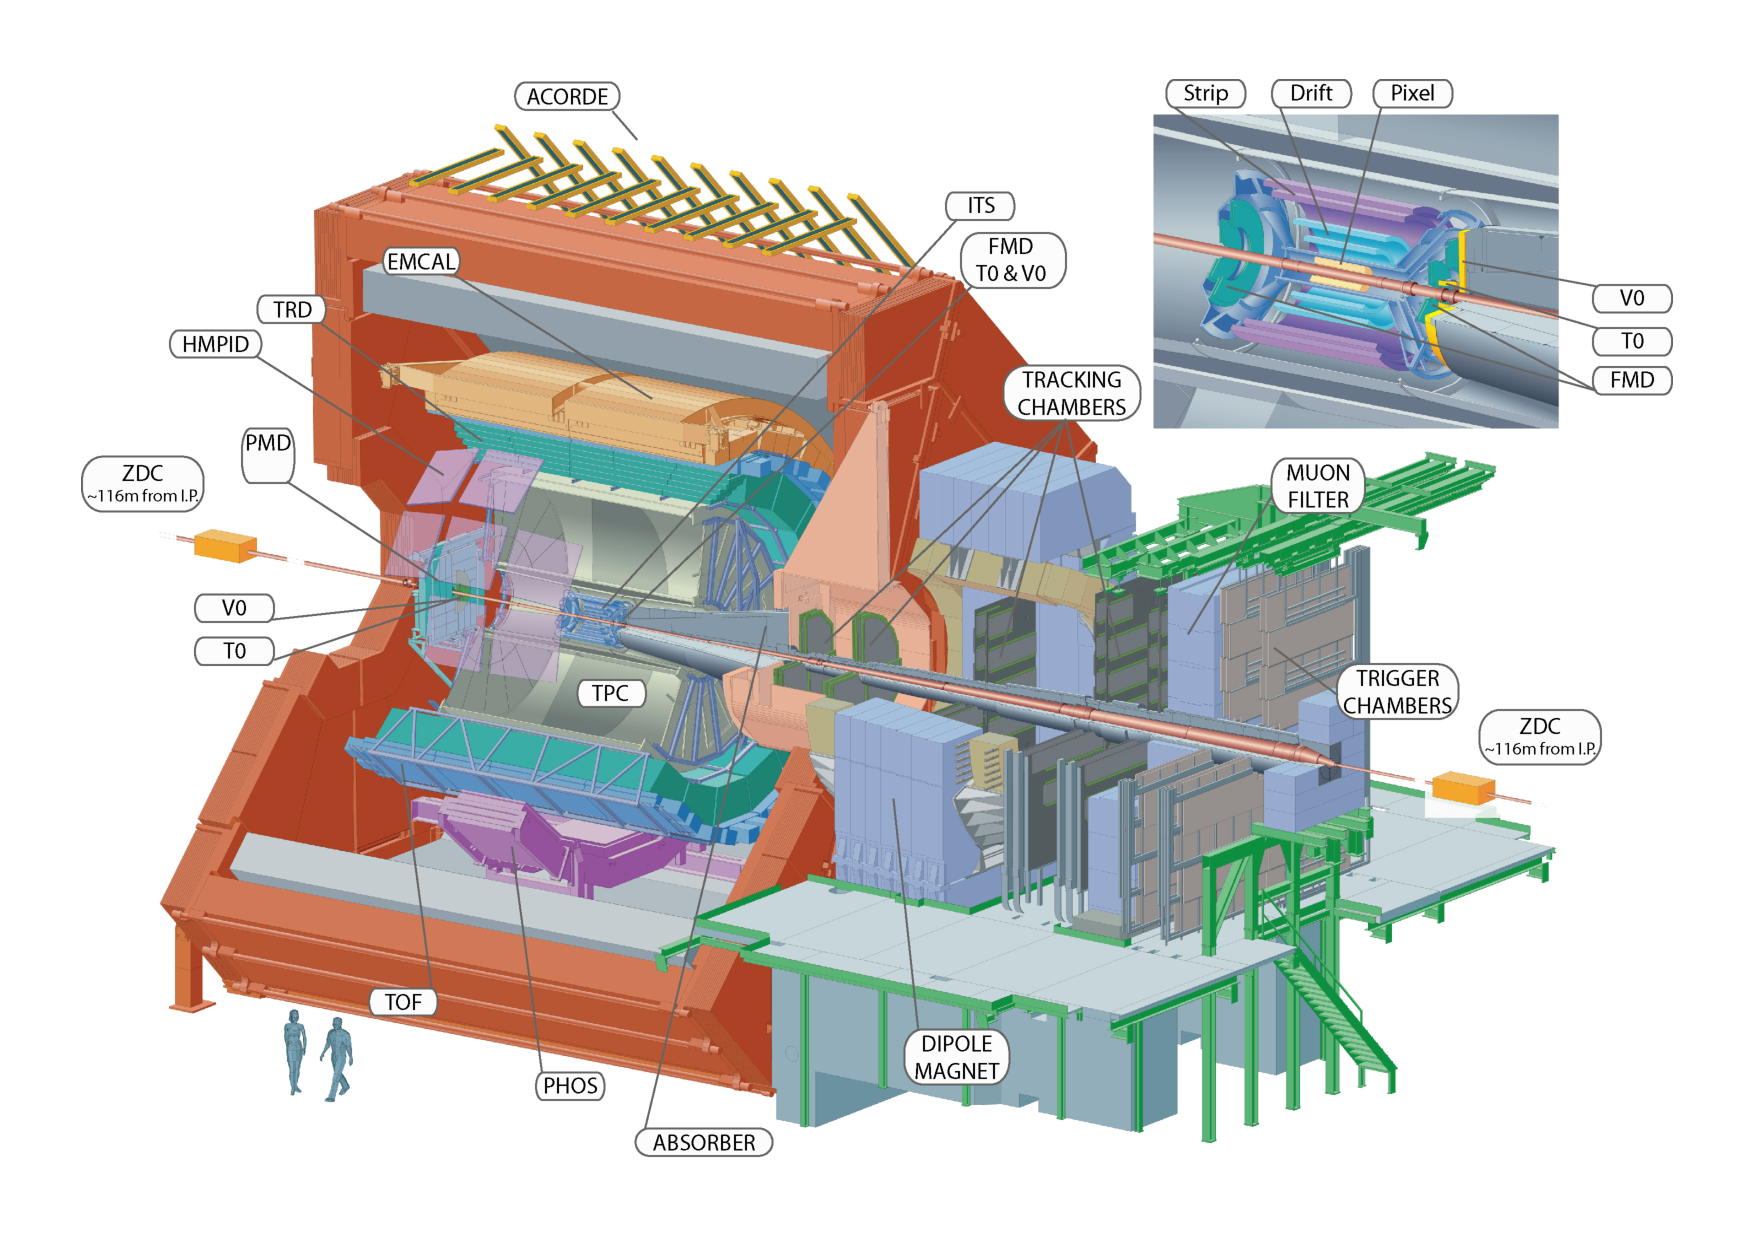
\includegraphics[width=14.cm]{./Version1/FigChapter4/FigureALICE}
\caption{ The ALICE detector}
\label{fig:alicedetector}
\end{center}
\end{figure}


The ALICE global coordinate system \cite{cite:ALICEcoord} is a right-handed orthogonal Cartesian system with the origin X, Y, Z = 0 at the centre of the detector. The three Cartesian axes are defined as follows: the X axis pointing towards the center of the LHC, the Y axis pointing upward and the Z axis parallel to the local mean beam line pointing in the direction opposite to the muon spectrometer. The azi- muthal angle increases counter-clockwise from the positive X axis ( $\Phi$= 0) to the positive Y axis (  $\Phi$ = $\pi$/2) with the observer standing at positive Z and looking at negative Z; the polar angle increases from the positive Z axis ($\theta$ = 0) to the X-Y plane ($\theta$ = $\pi$/2) and to the negative Z axis ($\theta$ = $\pi$).

In the following Sections more specific descriptions of the detectors used in the identification of the \xis baryons and in the determination of the characteristics of typical collisions will be given. \\

{\Large\textsl{ITS}}\\
The ITS \cite{cite:ALICE} (Figure \ref{fig:its}) is the barrel detector which is closest to the beam pipe. Its main purposes are:

\begin{itemize}
\item to contribute to the global tracking with the TPC by improving the angle and momentum resolution
\item to reconstruct the position of the primary interaction vertex
\item to reconstruct strange particle decays and secondary vertices from decays of heavy-flavor
\item to track and identify particles with momentum below 100 \mmass
\item to improve the momentum, impact parameter and angle resolution for the measurement of high \pt particles performed with the TPC
\item to reconstruct particles traversing dead regions of the TPC
\end{itemize}


\begin{figure}[htbp]
\begin{center}
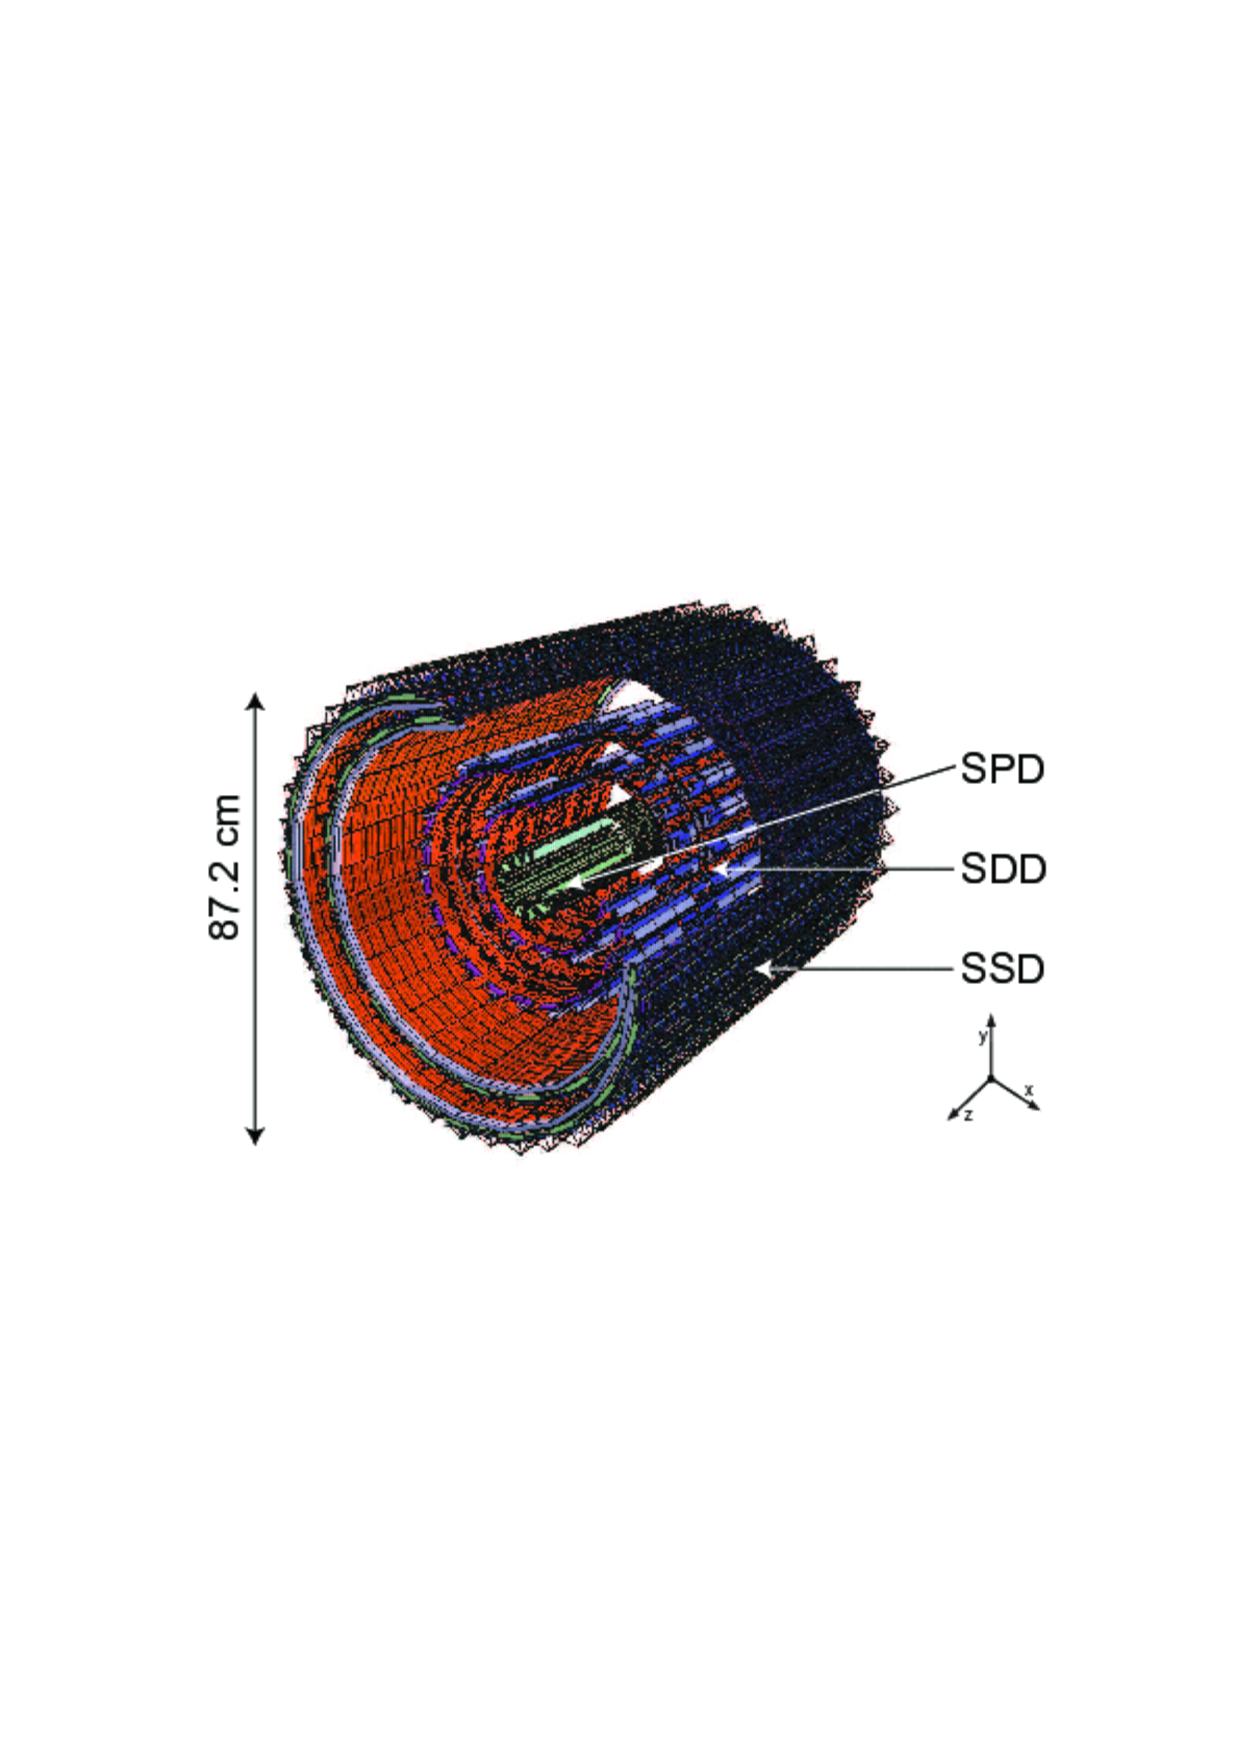
\includegraphics[width=12.cm]{./Version1/FigChapter4/FigureITS}
\caption{Schematic view of the ITS \cite{cite:ITS}}
\label{fig:its}
\end{center}
\end{figure}


The ITS encircles the beam pipe which is a 800 $\mu$m thickness cylinder shape with an outer diameter of 2.9 cm. It consists of six layers of silicon detectors placed at radii from $\sim$4 cm to $\sim$43 cm. The two innermost layers are Silicon Pixel Detectors (SPD), Silicon Drift Detectors (SDD) is placed in middle and the two outmost layers are Silicon micro-Strip Detectors (SSD). 

\begin{figure}[htbp]
\begin{center}
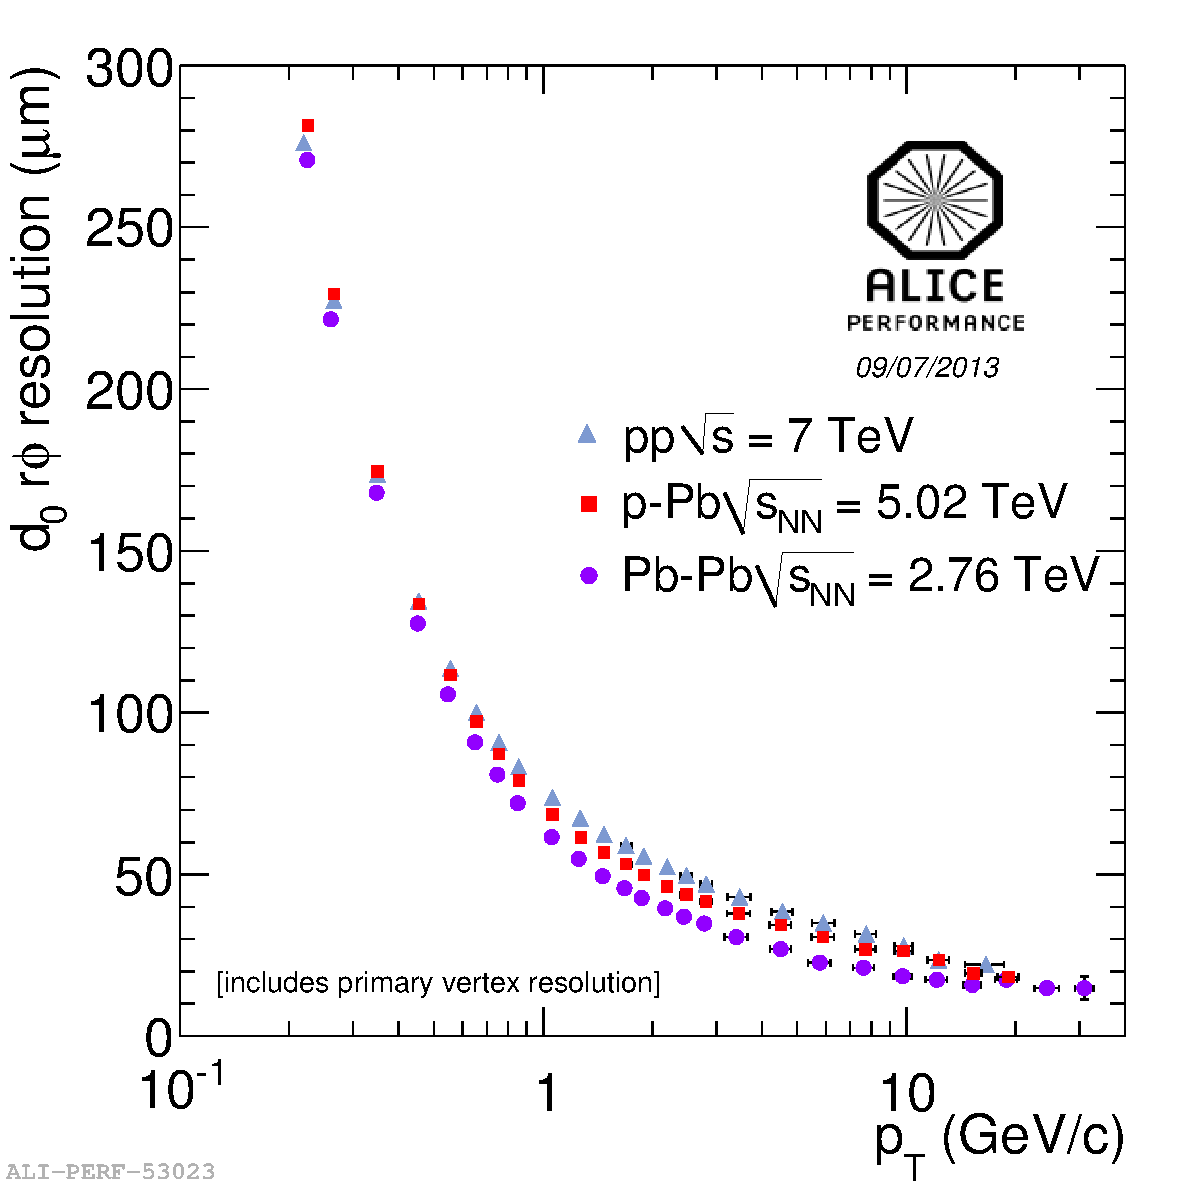
\includegraphics[width=10.cm]{./Version1/FigChapter4/ITSPerformance}
\caption{Track impact parameter resolution (r$\phi$) in the transverse plane as function of  \pt~for charged particle}
\label{fig:itsperformance}
\end{center}
\end{figure}


The amount of material in the detector has to be minimized because the momentum and impact parameter resolutions for low momentum particles are dominated by multiple scattering effects. The track impact parameter resolution as function of \pt~ is shown in Figure \ref{fig:itsperformance}. The ITS detector has a spatial resolution better than 70 $\mu$m in the (r$\phi$) for \pt $>$ 1 GeV/$c$. \\





{\Large\textsl{TPC}}\\

The TPC \cite{cite:TPC} (Figure \ref{fig:tpc}) is the main tracking detector of the central barrel optimized to measure charged particle momentum with good track separation, particle identification and vertex determination. In order to get the track in high multiplicity environment of Pb--Pb collisions, the TPC was designed to have an excellent tracking performance. For such reason, it was constructed as a drift chamber in 5 m cylindrical shape. The inner radius is r$_{in}$ $\sim$ 85 cm decided by the maximum acceptable track density and the most outer radius is r$_{out}$ $\sim$ 250 cm to minimize track length for which d$E$/d$x$ is $<$ 10\%. The volume of TPC is 90 m$^{3}$ and it is filled by Ne/CO$_{2}$/N$_{2}$. The readout chambers are installed at the two endplates of the cylinder. Their design is based on the Multi-Wire Proportional Chamber (MWPC) technique with pad readout. The TPC has good d$E$/d$x$ resolution as results it is able to identify particles with \pt $<$ 1 GeV/$c$ on a track-by-track basis.

\begin{figure}[htbp]
\begin{center}
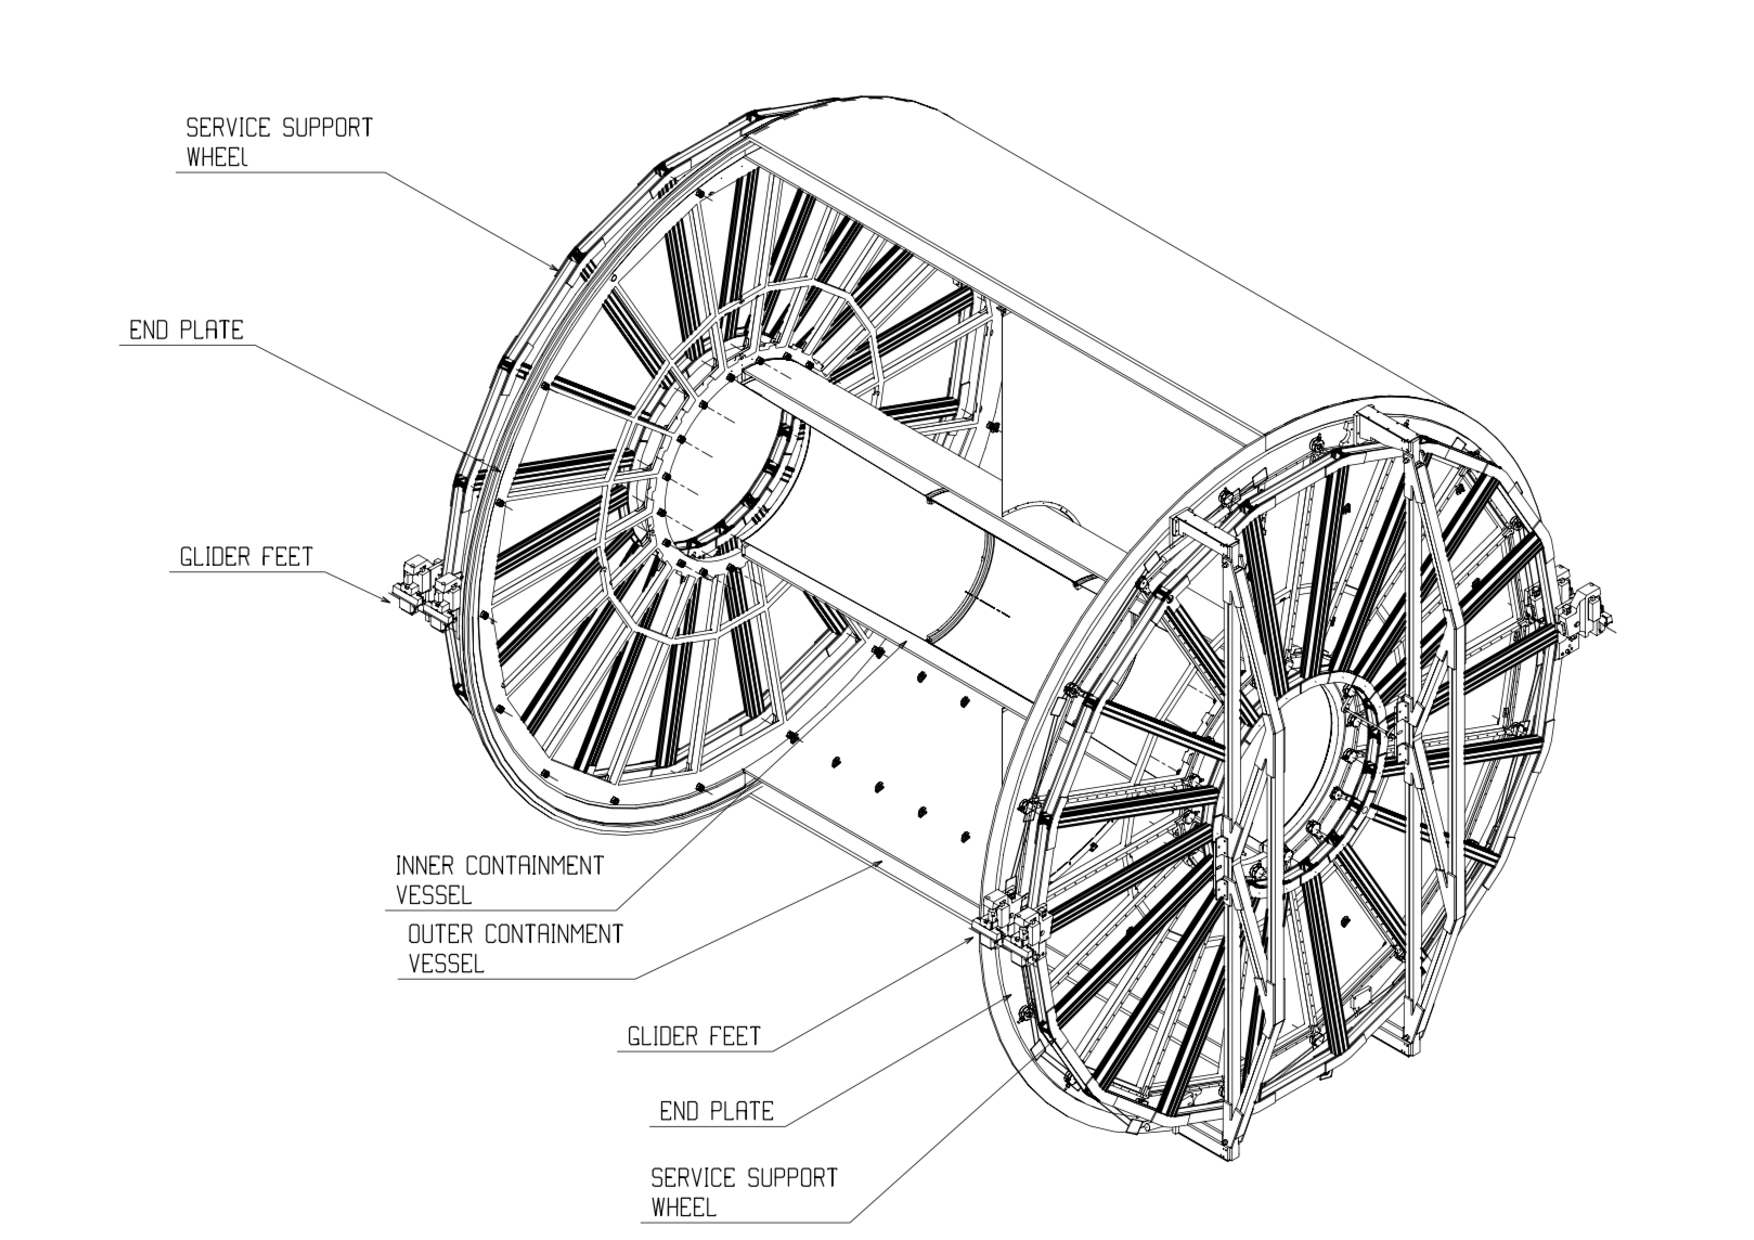
\includegraphics[width=10.cm]{./Version1/FigChapter4/FigureTPC}
\caption{Schematic view of the TPC}
\label{fig:tpc}
\end{center}
\end{figure}


The gas in the detector is ionized by charged particle traveling through the TPC. The measurement of this loss of energy is what we need to identify a particle. The physics observable in this case is the energy loss per unit length, within the matter crossed by the charged particle, which we call specific energy loss, also denoted by dE/dx. This is described by the Beth--Bloch equation, \ref{eq:BB}, that highlights the key of the identification technique: this observable depends only on the charge and on velocity ($\beta$) of the particle, which, in turn, depends only on the momentum and the mass of the ionizing particle. Since momentum is already known due to track curvature and charge is unitary for most measured tracks, measuring the dE/dx allows us to indirectly determine mass and thus determine the particle species.
The Bethe-Bloch equation gives the mean specific energy loss:
\begin{equation}\label{eq:BB}
- \langle\frac{dE}{dx}\rangle = k_{1} \cdot z^{2} \frac{Z}{A} \cdot \frac{1}{\beta^{2}}[\frac{1}{2}ln(k_{2}\cdot m_{e}c^{2}\cdot \beta^{2} \gamma^{2})-\beta^{2}+k_{3}]
\end{equation}

where $\beta\gamma$ = $\ensuremath{p}$/Mc and:
Z: atomic number of the ionized gas (in this case Ne/CO$_{2}$/N$_{2}$)\\
A: mass number of the ionized gas (g/mol)\\
m$_{e}$: electron mass\\
z: electric charge of the ionizing particle in unit of electron charge e\\
M: ionizing particle mass\\
$\ensuremath{p}$: ionizing particle momentum\\
$\beta$: ionizing particle velocity normalized to the light velocity c\\
$\gamma$ = 1/$\sqrt{1-\beta^{2}}$, Lorent factor\\
k$_{1}$, k$_{2}$, k$_{3}$: constants depending on the ionized medium\\ 


For a given ionizing particle mass hypothesis, a given momentum and a given length of the trajectory in the ionizing medium, the total charge deposited along the trajectory is subject to statistical fluctuations. This random variable follows a Landau distribution, that give us the opportunity to measure the mean value hdE/dxi. The long tail of the Landau distribution is usually truncated at 50\%-70\% of the collected signal. 

\begin{figure}[htbp]
\begin{center}
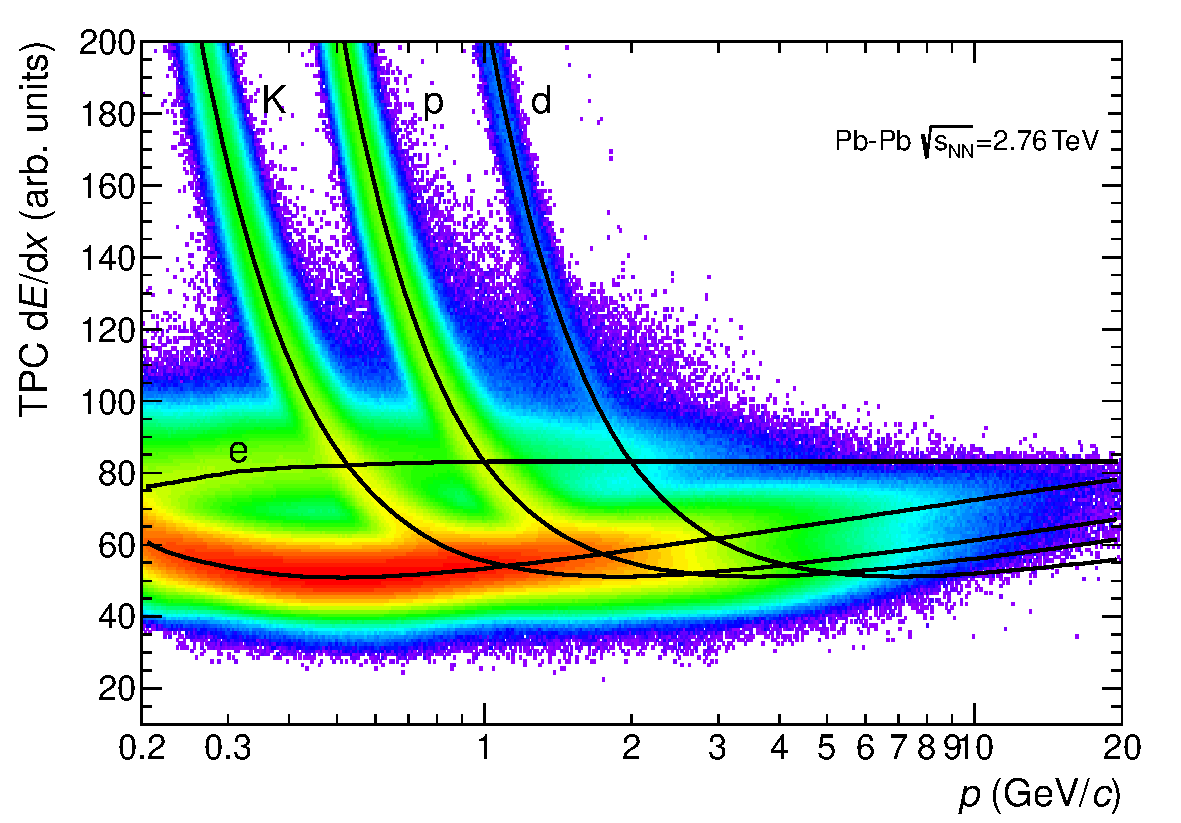
\includegraphics[width=10.cm]{./Version1/FigChapter4/TPCPID}
\caption{Specific energy loss (d$E$/d$x$) in the TPC as a function of particle momentum in Pb--Pb collisions at \snn= 2.76 TeV. The lines show the parametrisations of the expected mean energy loss.}
\label{fig:tpcpidPbPb}
\end{center}
\end{figure}

The specific energy loss in the TPC as a function of momentum is shown in Figure \ref{fig:tpcpidPbPb}. The different bands characteristic for e$^{\pm}$, $\pi^{\pm}$, K$^{\pm}$, p$^{\pm}$ are clearly visible. These are the evidence of the statistical distribution of the measured energy loss around the expected mean value. The expected value correspond to the prediction by a Bethe--Bloch experimental parametrization (superimposed as black lines in the Figure). For a track within the TPC the relevant quantity to be considered for PID is the difference between the specific energy loss measured by detector and the corresponding predicted value, by the Bethe-Bloch parametrization for a given measured momentum. If normalized to the resolution of the d$E$/d$x$ measurement in the TPC, this difference could be expressed in number of $\sigma$(see Equation \ref{eq:nsigma}). In this way it is possible to estimate more quantitatively the goodness of a mass hypothesis. This also gives us the possibility to choose the strictness we want to adopt in the identification of a particle (n$_{\sigma}$ , n = 2, 3, 4):

\begin{equation}\label{eq:nsigma}
n_{\sigma} = \frac{(dE/dx)_{measured}-(dE/dx)_{Bethe-Bloch}}{\sigma_{TPC}}
\end{equation}


{\Large\textsl{V0}}\\
The VZERO detector \cite{cite:V0} consists of two segmented arrays of plastic scintillator counters, called VZERO-A and VZERO-C, placed near the beam-pipe on each side of the interaction point: one at Z = 340 cm, covering the pseudo-rapidity range (2.8 $< \eta <$ 5.1), and the other at Z = -90 cm in front of the absorber, covering the pseudo-rapidity range (-3.7 $< \eta <$ -1.7). 

%Each of VZERO (A or C) consists of 32 channels distributed in 4 rings with separation of 45$^{\circ}$. The Wave-Length Shifting (WLS) fibers are embedded in both face of the detector. Clear fibers collect and transport the signal to photomultipliers 3 - 5 m far from the detector, inside the L3 magnet. The counters have a time resolution better than 1 ns. Their response is recorded in a time window of 25 ns around the nominal beam crossing time.

By measuring the relative time of flight, the VZERO reject background from beam-gas collisions. (see, Figure \ref{fig:v0}) The time of flight of particles coming from the interaction point to the VZERO-A is $\sim$ 11 ns while VZERP-C is 3 ns. If the beam-gas collision takes place outside the region between the two arrays, particles arrive 6 ns before or after the time of a beam-beam collisions. When the beam-gas collision takes place outside the region between the two arrays, particles arrive 6 ns before or after the time of a beam-beam collision as shown in Figure \ref{fig:v0time.}

\begin{figure}[htbp]
\begin{center}
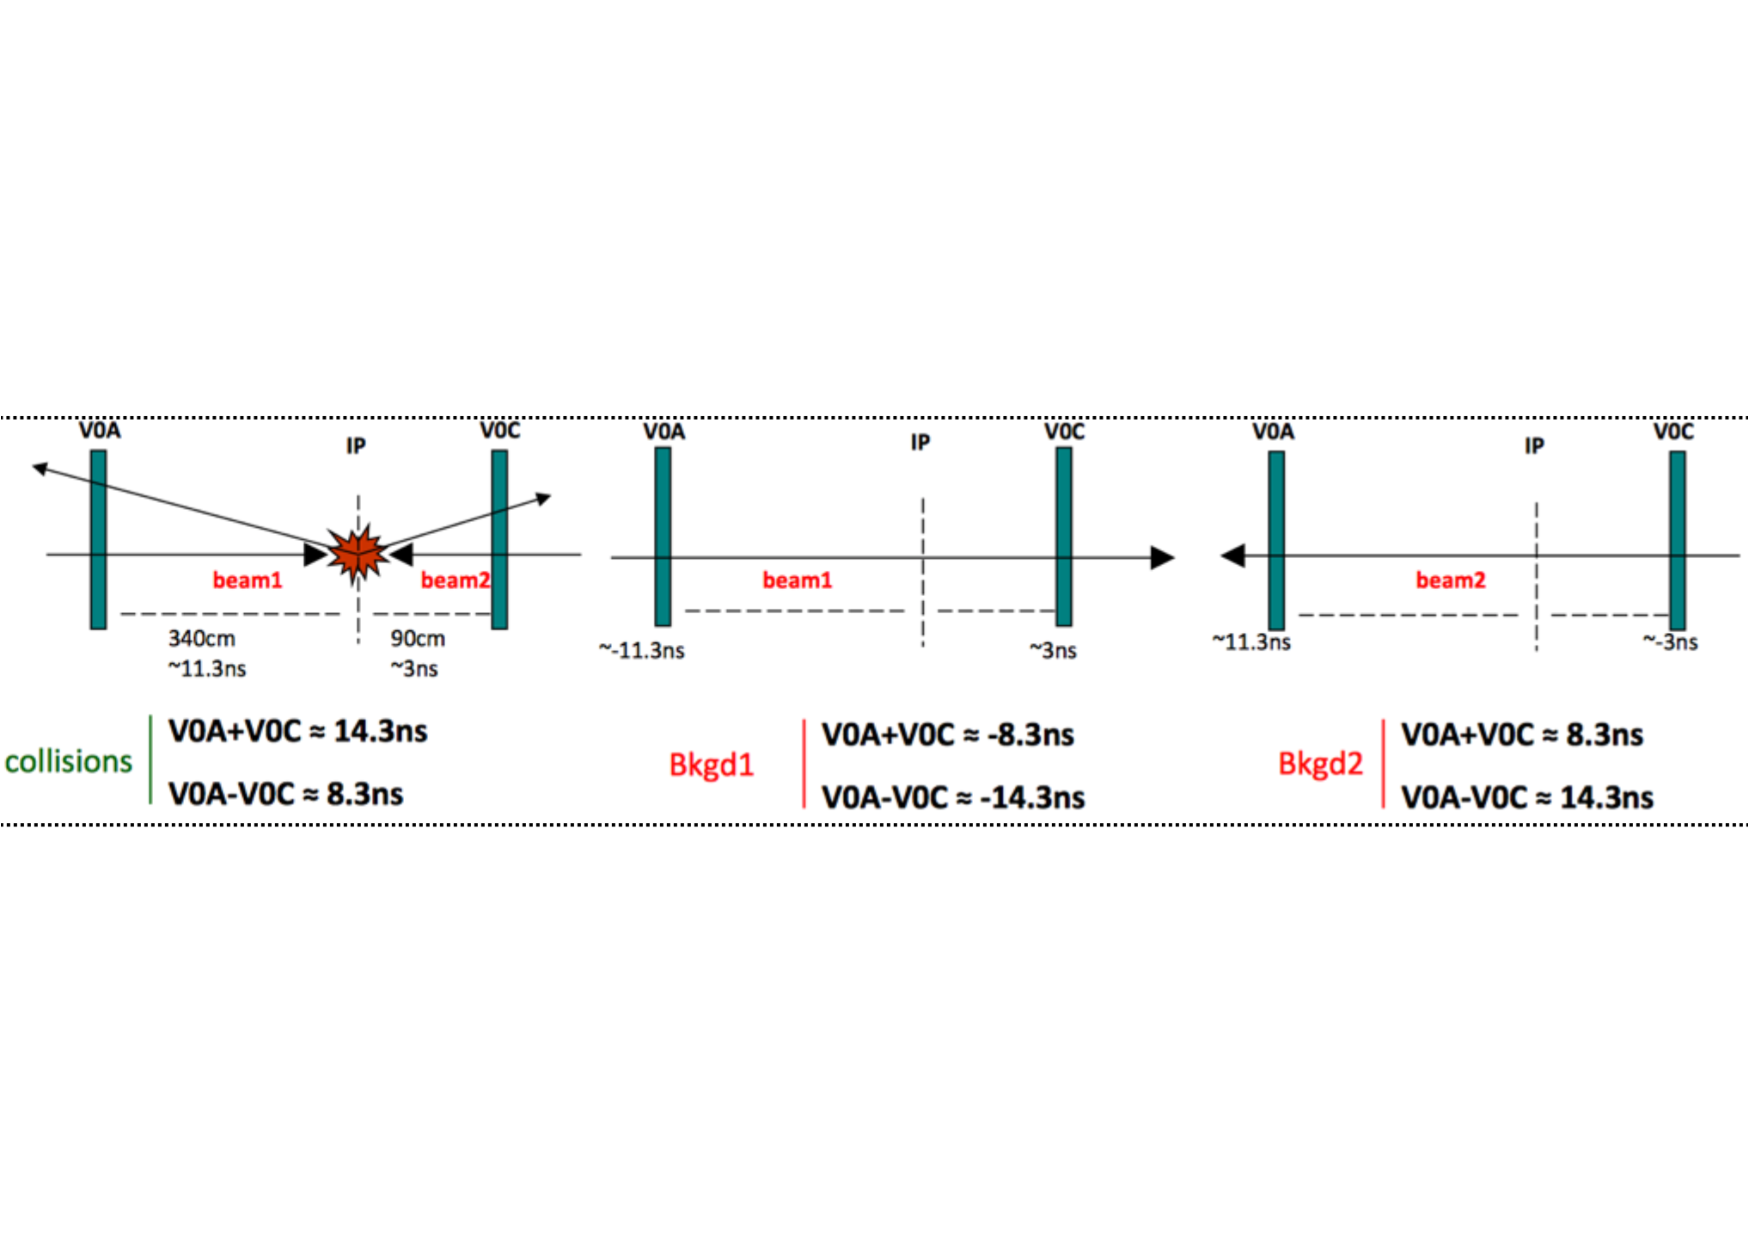
\includegraphics[width=14.cm]{./Version1/FigChapter4/V0time}
\caption{Sketch of events collisions at (8.3 ns, 14.3 ns) is shown in left, background from Beam 1 at (-14.3 ns, -8.3 ns) in in middel and background from Beam 2 at (14.3 ns, 8.3 ns) is in right.}
\label{fig:v0time}
\end{center}
\end{figure}

\begin{figure}[htbp]
\begin{center}
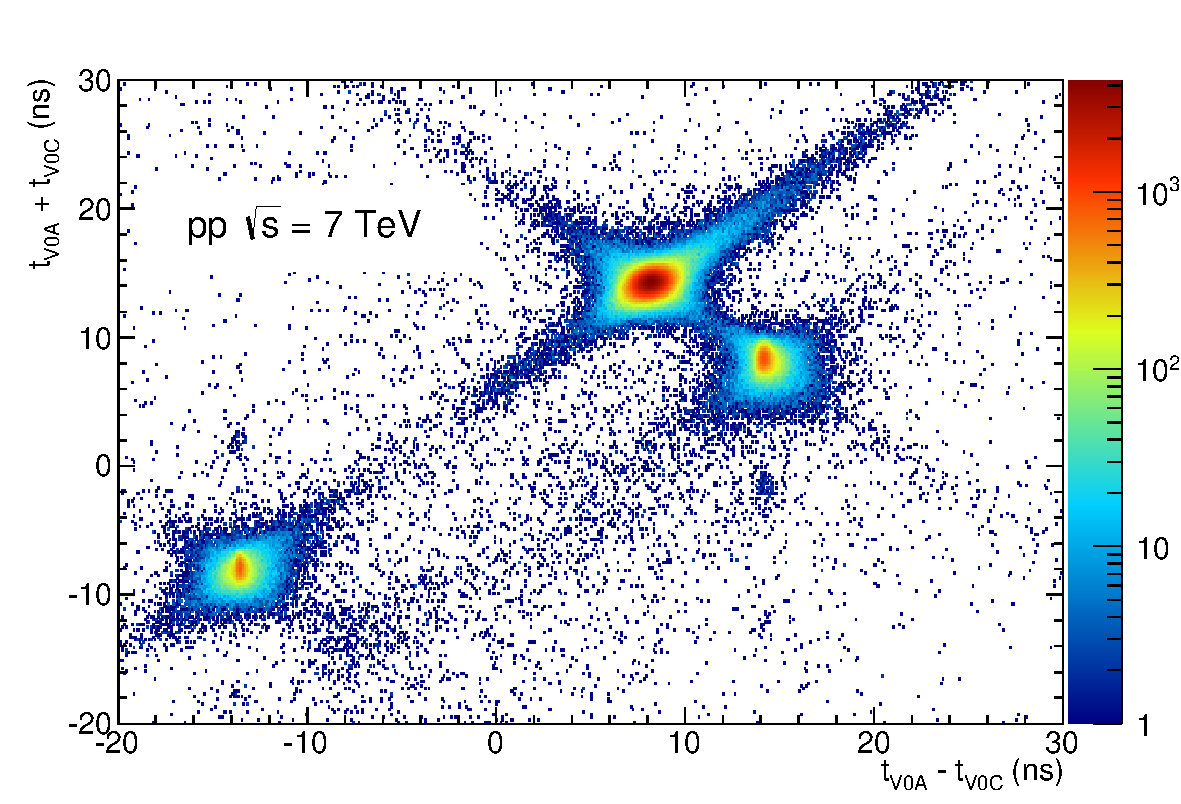
\includegraphics[width=10.cm]{./Version1/FigChapter4/FigureV0}
\caption{Correlation between the sum and difference of signal times in V0A and V0C. The signals in center come from beam-beam interactions, the signal in left is background from Beam1 and background from Beam2 is shown in right hand.}
\label{fig:v0}
\end{center}
\end{figure}



As the VZERO is a trigger detector, it will provide a minimum-bias trigger for all colliding systems to the central barrel detectors and different centrality triggers in p--Pb and Pb--Pb collisions (e.g. multiplicity, central and semi-central).  

The first parameter to be determined in A--A(p--A) collisions is the centrality(multipliciy). This is defined according to the value of the impact parameter, b, and provides a geometrical scale of the overlapping region between the colliding nuclei: a collision will be defined from central to peripheral, as the impact parameter increases. The centrality of a collision is not directly available and must be deduced from a combination of experimentally measured quantities and Monte Carlo simulations.
There are a number of observables that can be measured and used as centrality estimators. The charged-particle multiplicity N$_{ch}$ and the transverse energy E$_{\mathrm{T}}$ measured around mid-rapidity are measurable quantities related to the energy deposited in the interaction region (these are therefore related to N$_{part}$). These variables increase significantly increasing the centrality of the collisions. Another measurable quantity to estimate the centrality is the zero-degree energy EZDC, namely the energy carried by spectator nucleons N$_{spec}$ = 2A - N$_{part}$ = E$_{ZDC}$/E$_{A}$, where E$_{A}$ is the beam energy per nucleon.
Typically a measured distribution of one of the previous observables is mapped to the corresponding distribution obtained from phenomenological Glauber calculations. The Glauber model \cite{cite:glauber,cite:glauber1} uses a semi-classical approach: the A--A collision is assumed to be an incoherent superposition of N elementary nucleon- nucleon collisions. The main parameters of the model are the inelastic nucleon-nucleon collision cross-section  $\sigma_{n}$ and the nuclear density distribution $\rho$(r). In practice, the simulated distribution well reproduce the measured distribution or the latter is fitted with an analytical function. The experimental distribution can then be divided in classes with sharp cuts on the measured observable (E$_{ZDC}$, E$_{T}$ or N$_{ch}$). These "centrality" classes will correspond to well defined percentage of the integral of the distribution. A given centrality class in the measured distribution, corresponds to the same class in the simulated distribution, where the main geometrical variables (N$_{part}$, N$_{coll}$ and T$_{AA}$) can be determined. The number of classes that can be defined depends on the resolution achievable on the selection variable.
In the analysis described in this thesis the centrality(multiplicity) estimation is based on the measurement of the multiplicities from the VZERO scintillators \cite{cite:centralitypPb}\cite{cite:centralityPbPb}. This is the method that achieve the best centrality resolution: it ranges from 0.5\% in central to 2\% in peripheral collisions. Other methods, as the ones based on the E$_{ZDC}$ measurement or based on the estimate of the number of tracks in the SPD or TPC, are used to asses a systematic uncertainty on the centrality determination.
The distribution of the VZERO amplitudes is shown in Figure \ref{fig:centralityestimate} where the centrality(multiplicity) percentiles are also indicated. 

\begin{figure}[htbp]
\begin{center}
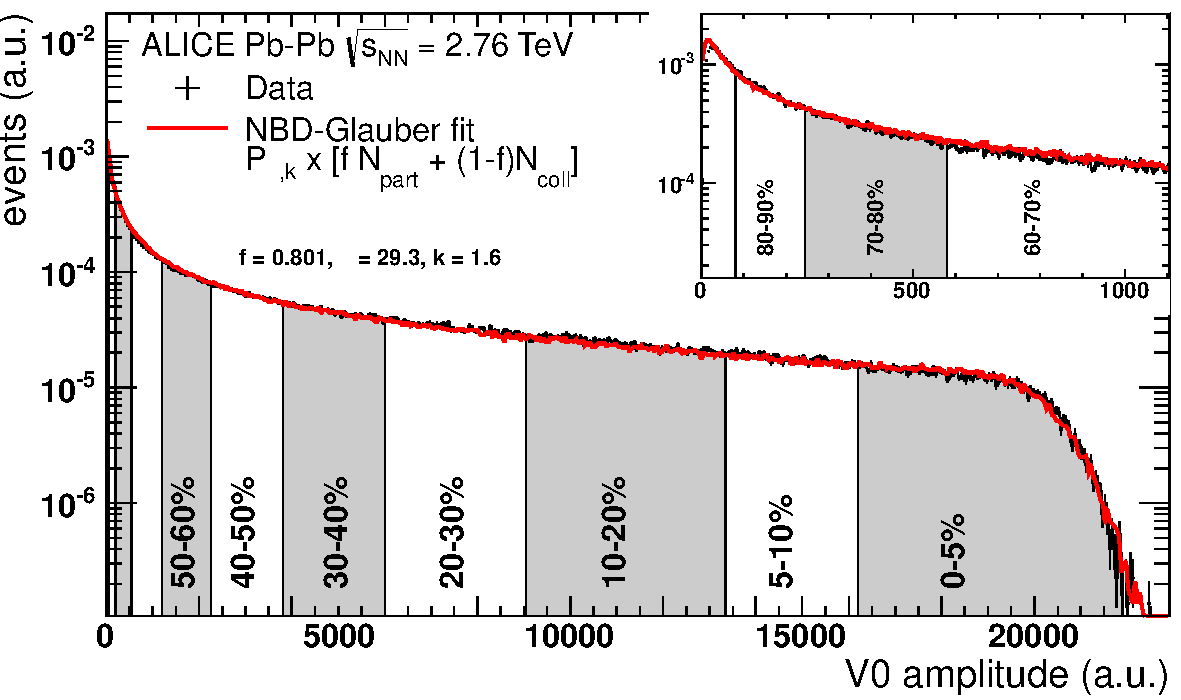
\includegraphics[width=12.cm]{./Version1/FigChapter4/CentralityPbPb}
\hspace{1.0cm}
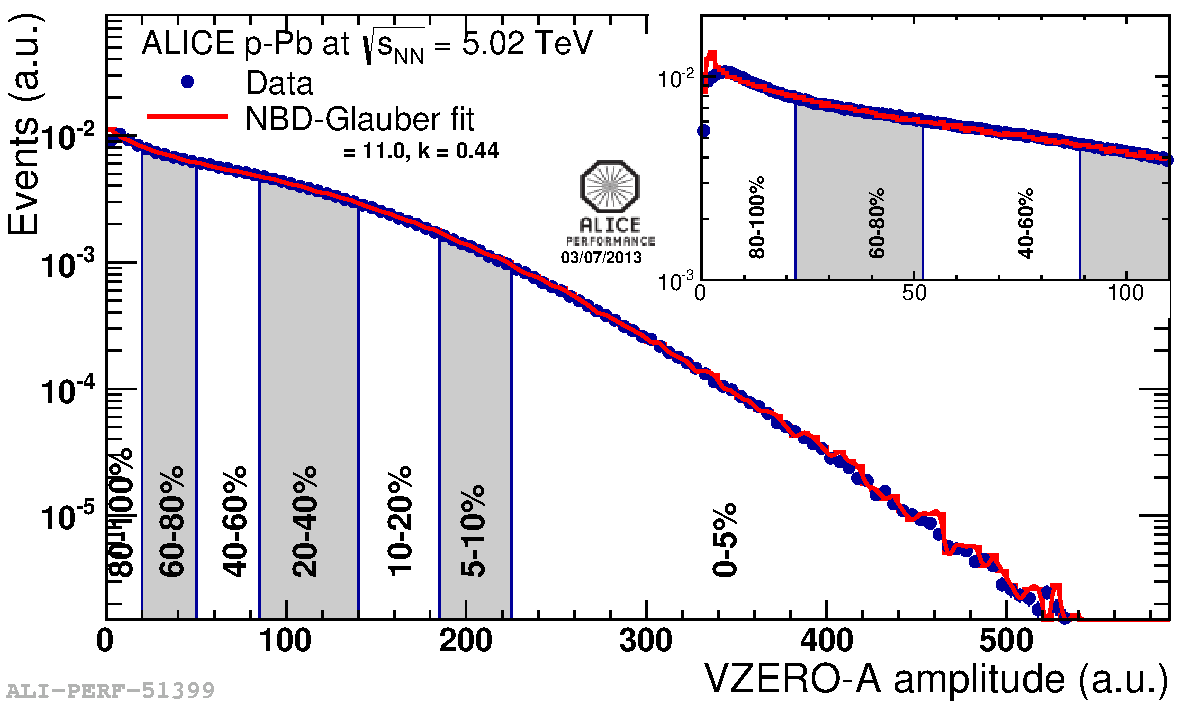
\includegraphics[width=12.cm]{./Version1/FigChapter4/CentralitypPb}
\caption{ Sume of V0A and V0C amplitude distribution in top and V0A amplitude distribution in bottom.}
\label{fig:centralityestimate}
\end{center}
\end{figure}

\newpage
\subsubsection{Data Acquisition (DAQ) and trigger system}\label{label:aliceDAQ}
The architecture of data acquisition is shown in Figure \ref{fig:daq}. The tasks of the ALICE DAQ system are the assembly of event informations from individual detectors into complete events (event building) as well as buffer- ing and export of assembled events to permanent storage. The DAQ is designed to process a data rate up to 1.25 GB/s in heavy-ion runs. Event building is done in two steps. Data from the detectors is received by Detector Data Links (DDLs) on Local Data Concentrators (LDCs). The LDCs assemble the data into sub-events that are then shipped to Global Data Collectors (GDCs). A GDC re- ceives all sub-events from a given event and assembles them into a complete event. These events are subsequently stored on a system called Transient Data Storage (TDS).

\begin{figure}[htbp]
\begin{center}
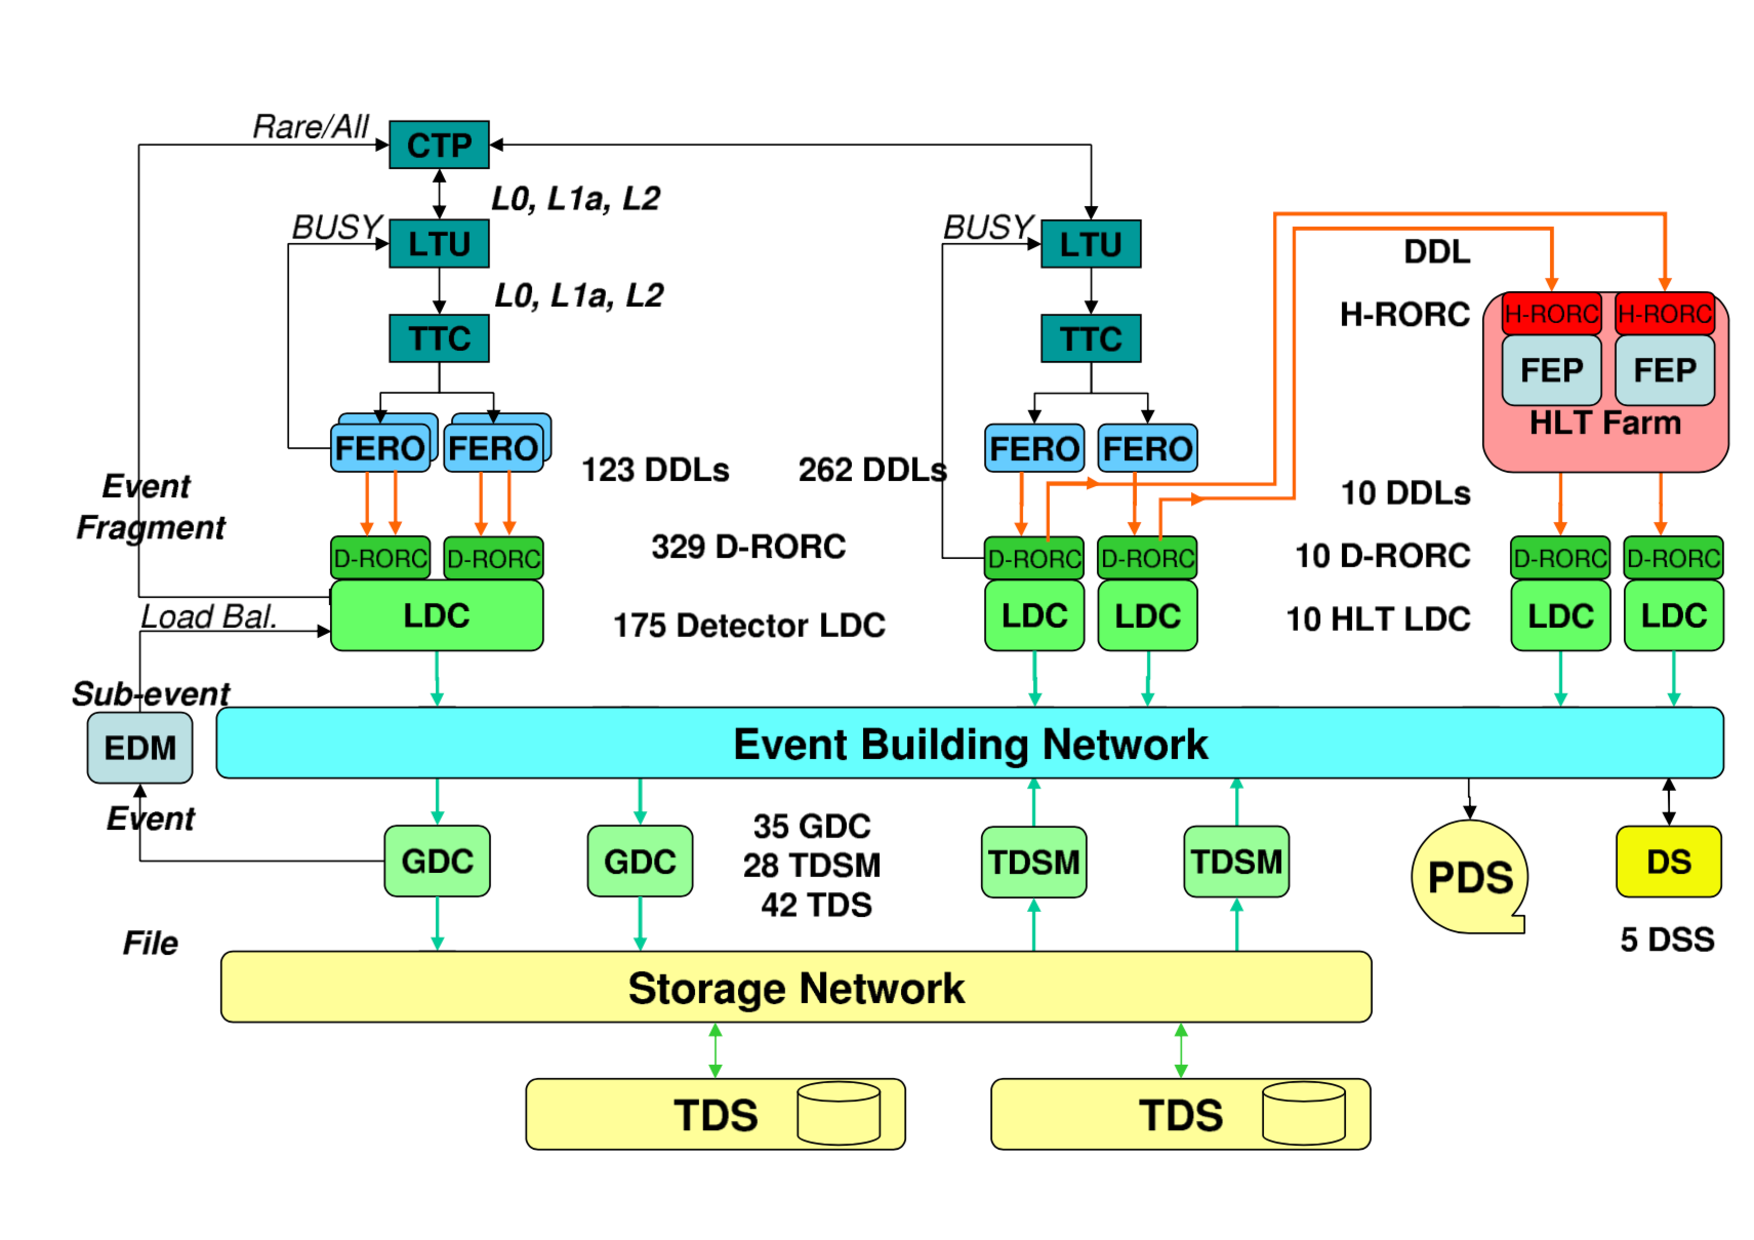
\includegraphics[width=14.cm]{./Version1/FigChapter4/FigureDAQ}
\caption{The overall architecture of the ALICE DAQ and the interface to the HLT system.}
\label{fig:daq}
\end{center}
\end{figure}

 ALICE can simultaneously take data in several partitions, where a set of detec- tors can store their outputs. Since a partition is a group of commonly controlled detectors, a given detector can only be active in one partition at a time. The ac- tive detectors in a given partition may be assigned to data taking groups called clusters, for which triggers can be defined. Therefore, upon a trigger only a sub- set of the whole partition may be read out. Furthermore, a triggering detector does not have to be necessarily part of the partition.
ALICE has a two-layer trigger architecture \cite{cite:daq}. The low-level trigger is a hardware trigger called Central Trigger Processor (CTP). The High-Level Trigger (HLT) is implemented as a pure software trigger. The CTP combines inputs from different trigger sources, namely the various detectors. These inputs are single signals, like a hit in the detector, or, can be the result of fast calculation performed directly in the detectors. The HLT allows the implementation of sophisticated logic for the triggering. In contrast to the CTP which governs the readout of the detectors, the HLT receives a copy of the data read out from the detectors and processes them.
The hardware trigger combines the trigger signals of the various detectors to decide if an event is accepted, that means it is read out and written to disk. Several trigger levels reduce the event rate depending on the input signals. The first level, called L0, is delivered after 1.2 ?s, while the second, called L1, after 6.5 ?s. The final trigger, L2, is delivered after 100 ?s, upon completion of the drift time in the TPC. Only after an L2 trigger the event is finally stored. The rates of different trigger classes are very different. By definition minimum-bias triggers have the highest rate; other triggers that look for rare signals are characterized by much lower rates. In order to cope with different scenarios, downscaling factors can be applied to the trigger classes individually, i.e. only every nth event fulfilling the trigger condition is read out. The total recording rate is limited by the maximum bandwidth of data that can be recorded to disk and tape.
The ALICE software trigger, called HLT, is a farm of multiprocessor computers. The aim is to have about 1000 PCs processing the data in parallel allowing an online analysis of the events. A trigger decision comes from the analysis of a more comprehensive set of information than what happens for the hardware trigger, giving the possibility to apply more sophisticated triggers. Examples include triggers on high energy jets or on muon pairs. Furthermore, the HLT can significantly reduce the event size by selecting regions of interest (partial readout of detectors) and by further compression of the data. The HLT receives a copy of the raw data and performs per detector reconstruction, partly aided by hardware coprocessors. Subsequently, the trigger decision is based on the global reconstructed event. In the same step a region of interest can be selected. In the last optional step, if the trigger decision is positive, the data are compressed. The trigger decision, partial readout information, compressed data, and the re- construction output is sent to LDCs and subsequently processed by the DAQ. In terms of the overall DAQ architecture, data sent by HLT is treated like stemming from a detector.

\newpage
\subsubsection{ALICE offline software frame work}\label{label:alicesw}
In order to reconstruct, analyze the raw data as well as the product simulated events, the computing power and resources are required. The ALICE uses decentralized computing system called Grid \cite{cite:grid}.
%{\Large\textsl{The AliEn Framework}}\\

The Grid paradigm is the unification of resources of distributed computing center, especially, computing power and storage, to provide them to users all over the World. It allows to provide their resources to wider community and the makes local resources to be shared with entire collaboration. Software which is implements the Grid is called Grid middleware. ALICE has developed a Grid middleware called AliEn \cite{cite:alien} that is set of tools and services. An ALICE user employs AliEn to connect to the ALICE Grid which is composed of a combination of general services that are provided by many Grid middleware solutions and ALICE-specific services provided by AliEn. Parts of the ALICE Grid are: i) a global file catalog that is a directory of files in storage elements distributed over the Globe, ii) the automatic matching of jobs for execution to a suitable location in one of the connected sites, iii) a shell-like user interface and iv) API9 services for the ROOT framework \cite{cite:aliroot}.


%{\Large\textsl{AliRoot Framework}}\\
AliRoot \cite{cite:ALICE} is the offline framework for simulation, alignment, calibration, reconstruction, visualization, quality assurance, and analysis of experimental and simulated data. It is based on the ROOT framework. Most of the code is written in C++ with some parts in Fortran that are wrapped inside C++ code. Re-usability and modularity are the basic features of the AliRoot framework. Modularity allows parts of the code to be replaced, with minimum or no impact on the rest (for example changing the event generator, the transport Monte Carlo or the reconstruction algorithms). This is achieved implementing abstract interfaces. In addition codes for each detector subsystem are independent modules with their specific code for simulation and reconstruction and the code can be developed concurrently with minimum interference. Re-usability is meant to maintain a maximum amount of backward compatibility as the system evolves.

\begin{figure}[htbp]
\begin{center}
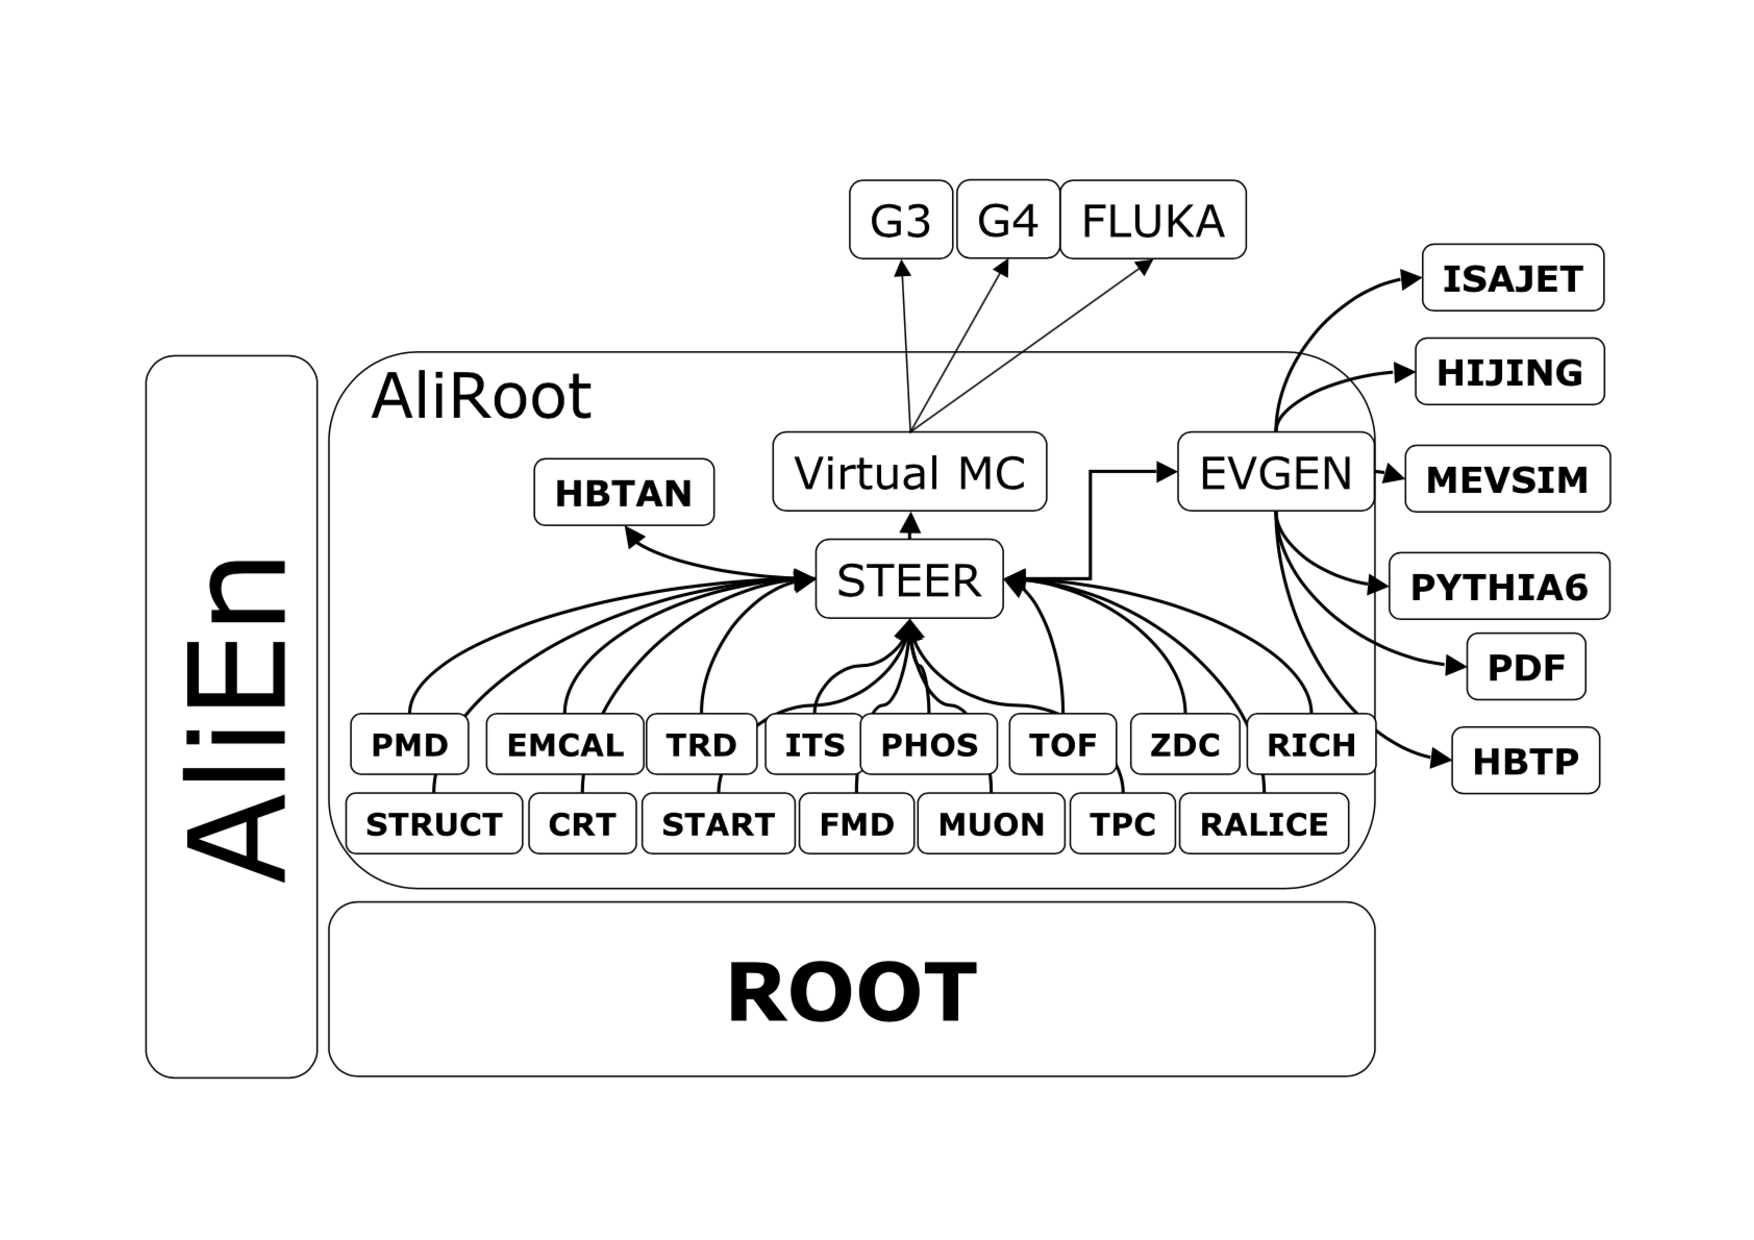
\includegraphics[width=16.cm]{./Version1/FigChapter4/FigureAliRoot}
\caption{Schematic view of the AliRoot framework}
\label{fig:aliroot}
\end{center}
\end{figure}

The central module of the AliRoot framework is STEER (Figure \ref{fig:aliroot}) which provides several common functions such as: steering of program execution for simulation, reconstruction and analysis; general run management, creation and destruction of data structures, initialization and termination of program phases; base classes for simulation, event generation, reconstruction, detectors elements.
For event simulation the framework provides the following functionality:

\newpage

%\section{The ALICE detector}
%\subsection{The Large Hadron Collider}
%\subsection{The ALICE project}
%\subsubsection{ALICE detector}
%\subsubsection{Data Acquisition (DAQ) and trigger system}
%\subsubsection{ALICE offline software frame work}

\section{Measurement of \xis production in p--Pb and Pb-Pb}\label{sec:pPbPbPb}
The measurement of hyperon resonance production in p--Pb collisions helps to disentangle cold nuclear matter effects from genuine hot medium effects and contribute to the study of the system size dependence of re-scattering and regeneration in the hadronic phase. And the measurement in ultra-relativistic heavy-ion collisions such as Pb--Pb collisions, allows to study the properties of hadronic medium and different stage of its evolution. 
In order to study the particle production mechanism in the hadronic phase between the chemical and kinetic freeze-out, the \xis resonance at mid-rapidity($-0.5<y_{\mathrm{CMS}}<0$) is measured in p--Pb collisions \snn = 5.02  TeV and in Pb--Pb collisions with $|y|<$0.5 at \snn 2.76 TeVwith the ALICE by the reconstruction of hadronic decay into $\Xi\pi$.

\subsection{\xis-reconstruction}\label{sec:Reconstruction}
The \xiss production in p--Pb and Pb--Pb collisions at mid-rapidity has been studied in different multiplicity and centrality classes, from peripheral to central collisions including minimum bias events. The analysis is based on the invariant mass of the reconstructed pairs which might be the decay of a \xiss baryon into charged particles. The daughter particles which is decay products are identified as oppositely charged $\Xi$ and $\pi$ among the tracks reconstructed in the central barrel. In section \ref{sec:Selection}, the event selection and track selection  applied in this analysis, and the particle identification is explained. Then, the raw yield from signal is extracted by integrating the fit on the background-subtracted invariant mass distribution of $\Xi$$\pi$ in several transverse momentum. To obtain the corrected \pt-spectra, the raw yields are corrected for acceptance and efficiency (Acc $\times$ $\epsilon_{rec}$)(pt) which is computed using Monte Carlo simulation. By dividing for the number of the events in each multiplicity and centrality classes, the normalization on the spectra is performed. 



\subsubsection{Data sample and event selection}\label{sec:Selection}
A description of the ALICE detector and of its performance during the LHC Run 1 (2010--2013)
can be found in \cite{cite:ALICE, cite:ALICEPerformance}. The data sample in the analysis from Pb--Pb collisions with energy of \snn =2.76 obtained during 2011 and the sample of p--Pb run at \snn = 5.02 TeV was recorded in 2013. 

Due to the asymmetric energies of the proton (4 TeV) and lead ion (1.57 A TeV) beams, the centre-of-mass system in the nucleon-nucleon frame is shifted in rapidity by $\Delta y_{\mathrm{NN}}$ = 0.465 towards the 
direction of the proton beam with respect to the laboratory frame of the ALICE detector \cite{cite:KphipPb}. 
For the analysed p--Pb data set, the direction of the proton beam was towards the ALICE muon spectrometer, the so-called ``C'' side, standing for negative rapidities; conversely, the Pb beam circulated towards positive rapidities, labelled as ``A'' side in the following. The analysis in this paper was carried out at midrapidity, 
in the rapidity window $-0.5 < y_{\mathrm{CMS}} <$ 0.

The minimum bias trigger during the p--Pb run was configured to collect events by requiring a logical OR of signals in V0A and V0C \cite{cite:ALICEPerformance}, two arrays of 32 scintillator detectors covering the full azimuthal angle in the pseudo-rapidity regions 2.8 $< \eta_{\mathrm{lab}} <$ 5.1 and $-3.7 < \eta_{\mathrm{lab}} < -1.7$, respectively~\cite{cite:rapidity}. In the data analysis it was required to have a coincidence of signals in both V0A and V0C to remove the events from single-diffractive and electromagnetic interactions. 

Out of this sample in p--Pb collision events about 109.3 million events, 93.9 million events pass the following selection criteria and have been used for the analysis.  %This left only Non-Single Diffractive (NSD) events, which amount for a total of 109.3 million events, in the Minimum-Bias sample($\sim$ 111.1 million events) corresponding to an integrated luminosity of about 50 $\mu$b$^{-1}$. 

The Pb--Pb collisions data sample was selected by online centrality trigger requiring a signal in the forward V0 detectors\cite{cite:centralityPbPb}  to record enhanced data in central collision. The data consists of 24.8 million events in most central collisions (0-10\%), 21.8 million events in semi-central collisions (10-50\%) and 3.5 million events with minimum-bas trigger (0-90\%). Among 49.6 million events in total, 43.0 million events have been analyzed as passed the criteria below. 



\begin{itemize}
\item Events with z-position of primary vertex (V$_{z}$) within $\pm$ 10 cm of the center of TPC/ITS
\item Rejection of pile-up event 
\item Requiring primary tracks to have at least one hit in SPD
\item p--Pb: multiplicity ranges in percentile (V0A): 0-20\%, 20-40\%, 40-60\%, 60-100\% and MB(0-100\%) 
\item Pb--Pb: centrallity classes (V0A and V0C): 0-10\%, 10-40\%, 40-80\% and MB (0-80\%)  
\end{itemize}


The distribution of the V$_{z}$ of the accepted events in p--Pb collision is reported on left panel in Figure \ref{fig:VzDistribution} and corresponding figure but obtained from Pb--Pb collisions is shown on right panel in Figure. \ref{fig:VzDistribution}. Events with $|$V$_{z}|<$10 cm have been used to make ensure that the tracks have been obtained from uniform acceptance in the central pseudo-rapidity region, $|\eta|<$0.8, where the analysis is performed. This cut reduces the total number of events to 97.5 million events, that is the $\sim$89.2\% of the initial sample in p--Pb collisions and 43.04 million events which is $\sim$86.8\% of the initial sample in Pb--Pb collisions are survived.

%The number of events before and after the each event selection stages are written in Table \ref{table:NEvent}. 

\begin{figure}[htbp]
\begin{center}
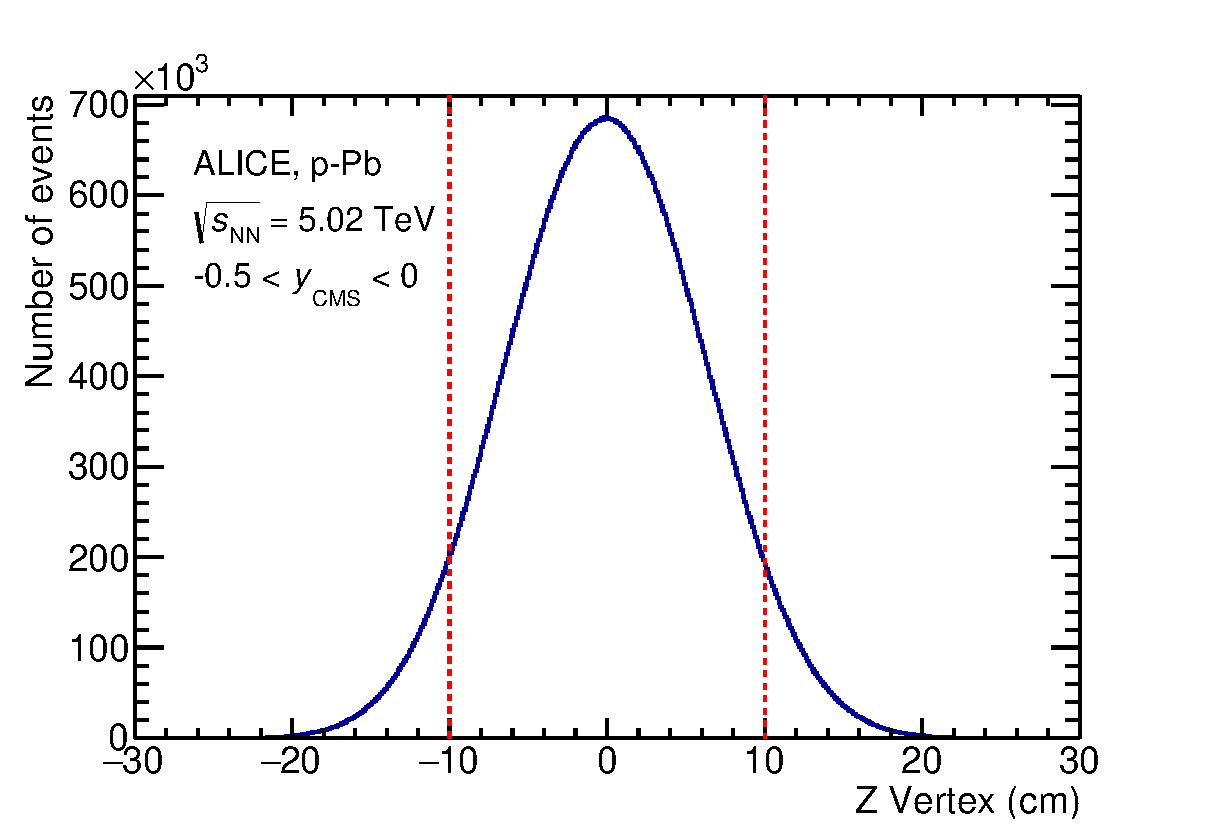
\includegraphics[width=7.cm]{./Version1/FigChapter5/Selection/pPbVertexZ.eps}
\hspace{0.5cm}
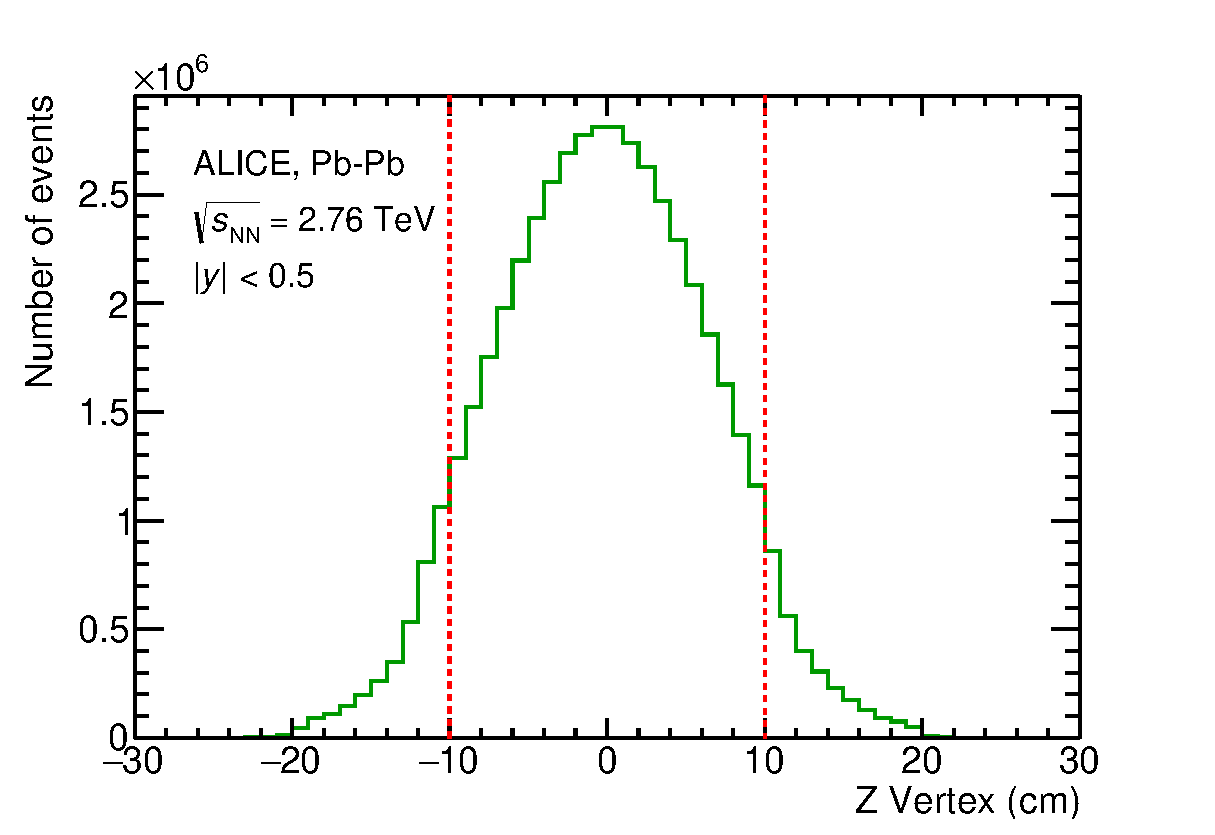
\includegraphics[width=7.cm]{./Version1/FigChapter5/Selection/PbPbVertexZ.eps}
\caption{Distribution of vertex-z position from the accepted events in p--Pb collision(Left) and in Pb--Pb collisions(Right). The red dashed line indicates vertex cut }
\label{fig:VzDistribution}
\end{center}
\end{figure}

%\begin{table}[htp]
%\begin{center}
%\begin{tabular}{|c|c|c|c|}
%\hline
%Event selection stage & number of events & percentage\\
%\hline
%\hline
%Original number of events &111.1 $\times$ 10 $^{6}$ &100.0\% \\
%\hline
%Number of triggered events (kINT7) &109.3 $\times$ 10 $^{6}$ &98.4\% \\
%\hline
%Events after PV position cut ($|$Vz$|$ $<$ 10 cm) & 97.5 $\times$ 10 $^{6}$ &87.8\% \\
%\hline
%Events after reject pile-up& 94.5 $\times$ 10 $^{6}$& 85.1\%\\
%\hline
%Events after number of SPD cluster cut ($\geq 1$)& 93.9 $\times$ 10 $^{6}$ &84.5\% \\
%\hline
%\end{tabular}
%\caption{Number of events at different selection stages.}\label{table:NEvent}
%\end{center}
%\end{table}




 Fig. \ref{fig:pPb:Centrality} shows the multiplicity distribution of the accepted events in p--Pb collision divided in bins of percentile. The each color on the histogram indicate the multiplicity ranges used in this analysis. Corresponding events for each multiplicity range are in Table \ref{table:NCentralityEvent}. 
 

\begin{figure}[htbp]
\begin{center}
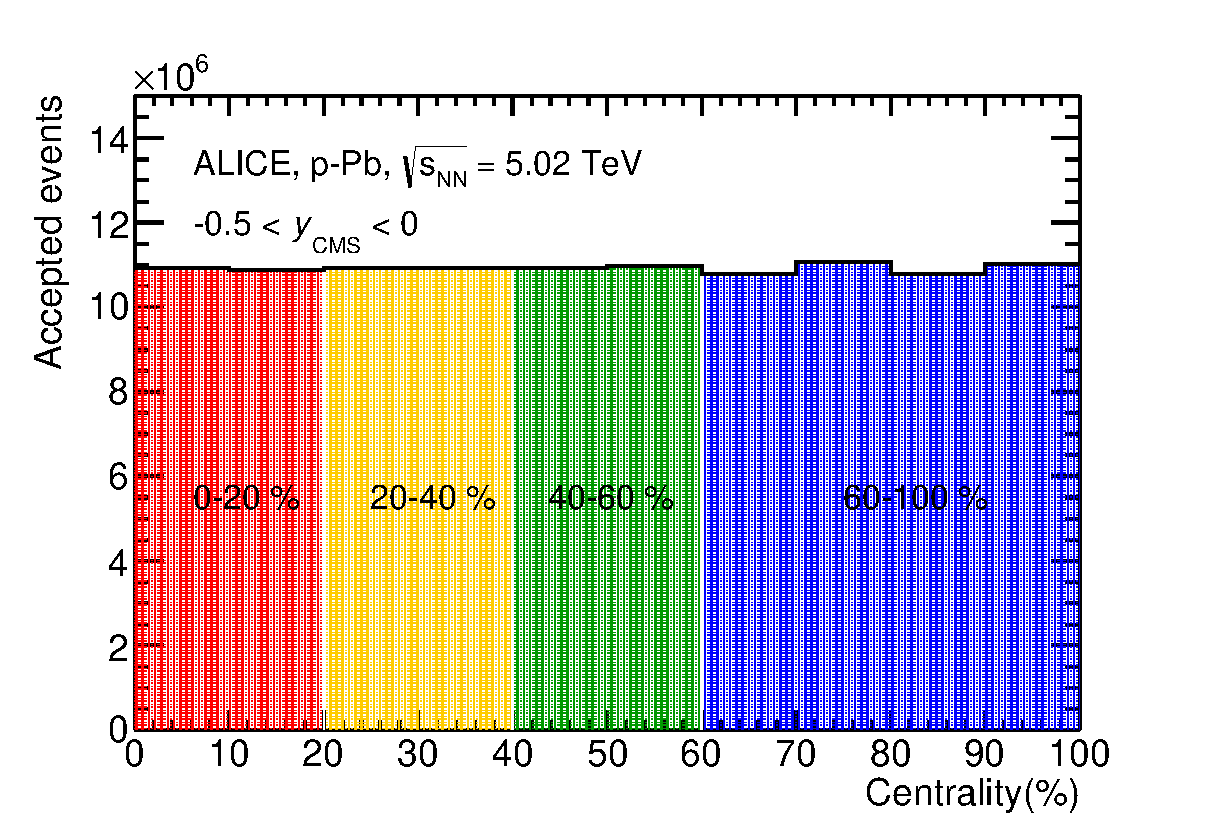
\includegraphics[width=10.cm]{./Version1/FigChapter5/Selection/pPbCentrality.eps}
\caption{ Multiplicity distribution of accepted events in p--Pb collision in percentile. The each color and labels define the four intervals in which the analysis in performed.}
\label{fig:pPb:Centrality}
\end{center}
\end{figure}

The distribution of centrality in each trigger used to select the events in Pb--Pb collision is shown in Fig. \ref{fig:PbPb:Centrality} and the reason why the centrality has step structure is that there are three different trigger classes classified by the amplitude threshold on VZERO detector.
Because the distribution of events as function of centrality is not a flat, this may lead to additional bias, in particular when one needs to combine the results from different triggers. For example, events from 40-80\% centrality bin have bias with high statistics in 40-60\%. In order to avoid this effect, we have applied a flattening procedure to have flat distribution of events as function of centrality. 
A brief explanation of the method is below : 

\begin{enumerate}
\item Histograms are obtained for the effective mass distribution in 1\% centrality bins and for the centrality distribution
\item The effective mass distributions are scaled in each 1\% centrality bin by a factor: \\
Factor = N{\footnotesize event in 20-40\%} / 20 / N{\footnotesize event in current 1\% bin}
\item Each bin in the centrality distribution is scaled using the factor described above
\item Histograms are added for centrality bins of interest: 0-10\%, 10-40\%, 40-80\%, 0-80\%
\end{enumerate}

The resulting number of events in each centrality classes is summarized in Table \ref{table:NCentralityEvent}.

\begin{figure}[htbp]
\begin{center}
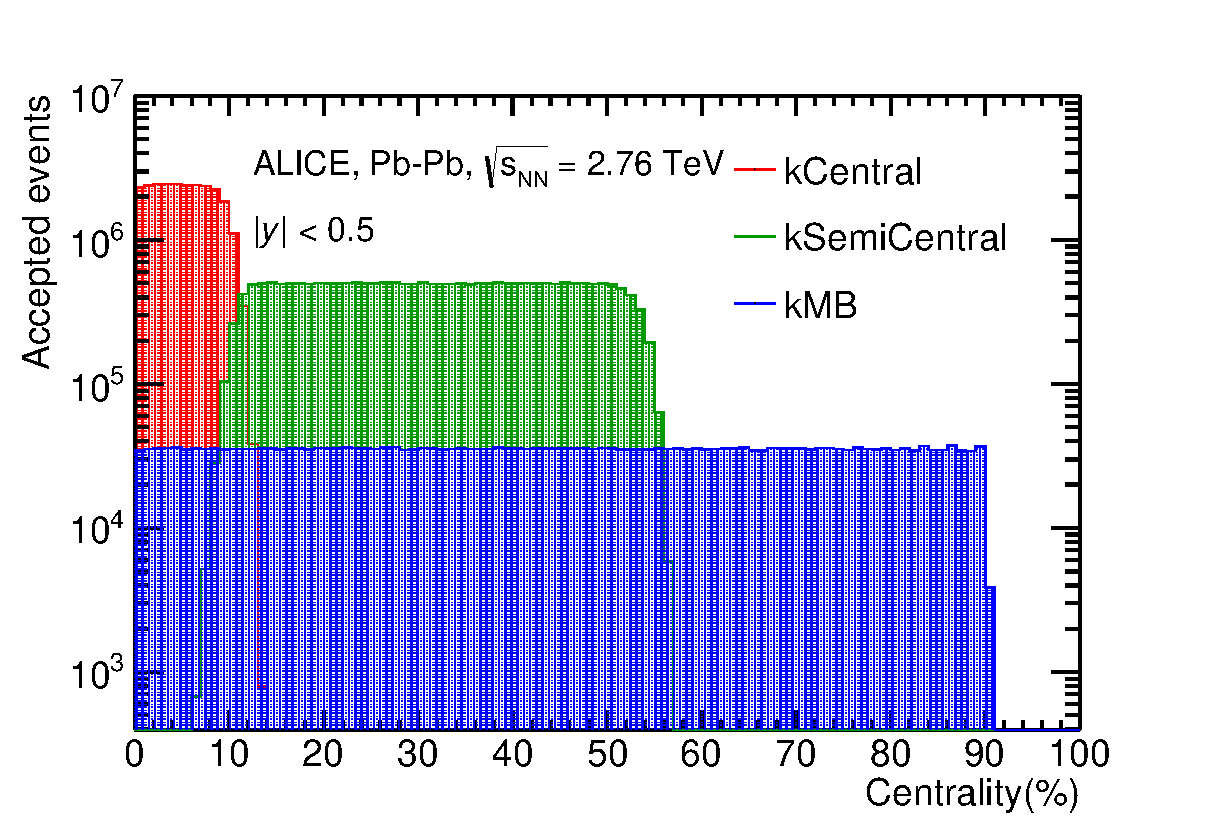
\includegraphics[width=10.cm]{./Version1/FigChapter5/Selection/PbPbCentrality.eps}
\caption{ Centrality distribution of three different trigger classes.}
\label{fig:PbPb:Centrality}
\end{center}
\end{figure}


\begin{table}[h!]
\centering
\begin{tabular}{lll}
\hline

p--Pb &   0-20\% &21.82 $\times$ 10 $^{6}$ \\
& 20-40\% &21.86 $\times$ 10 $^{6}$\\
& 40-60\% &21.91 $\times$ 10 $^{6}$ \\
& 60-100\% &43.68 $\times$ 10 $^{6}$ \\

\hline \noalign{\smallskip}

Pb--Pb& 0-10\%   & 5.58 $\times$ 10 $^{6}$ \\
& 10-40\%    & 16.73 $\times$ 10 $^{6}$ \\
& 40-80\% & 22.31 $\times$ 10 $^{6}$ \\
\hline\noalign{\smallskip}
\noalign{\smallskip}
\end{tabular}
\caption{Number of accepted and analyzed events per multiplicity/centrality interval}\label{table:NCentralityEvent}
\end{table}


\newpage
\subsubsection{Track and topological selection}\label{sec:Cut}

In comparison with the $\Xi^{*0}$ analysis carried out in pp collisions 
at $\sqrt{s}$ = 7 TeV~\cite{cite:Xi_pp}, track and topological selections were revised 
and adapted to the p--Pb dataset. Pions from strong decays of $\Xi^{*0}$ were selected
according to the criteria for primary tracks. As summarized in Table~\ref{tab:primary_selections}, 
all charged tracks were selected with \pt $>$ 0.15~ \gmom~ and $|\eta_{\mathrm{lab}}| <0.8$, as 
described in Ref.~\cite{cite:ALICEPerformance}. The primary tracks were chosen with the Distance of 
Closest Approach (DCA) to PV of less than 2 cm along the longitudinal direction (DCA$_z$)  and lower 
than 7$\sigma_r$ in the transverse plane (DCA$_r$), where $\sigma_r$ is the resolution of DCA$_r$. The 
$\sigma_r$ is strongly \pt-dependent and lower than 100 $\mu$m for 
$\pt >$~0.5~\gmom~\cite{cite:ALICEPerformance}. To ensure a good track reconstruction quality, 
candidate tracks were required to have at least one hit in one of the two innermost layers (SPD) of 
the ITS and to have at least 70 reconstructed points in the Time Projection Chamber (TPC), out of a 
maximum of 159. The Particle IDentification (PID) criteria for all decay daughters are based on the requirement 
that the specific energy loss (d$E$/d$x$) is measured in the TPC within three standard deviations 
($\sigma_\mathrm{TPC}$) from the expected value (d$E$/d$x_{\rm{exp}}$), computed using a Bethe-Bloch 
parametrization~\cite{cite:ALICEPerformance}.
\begin{table}[h!]
\centering
\begin{tabular}{lll}
\hline

Common track &  $|\eta_{\mathrm{lab}}|$ & $<0.8$ \\
 selections & \pt & $> 0.15$ GeV/$c$ \\
& PID $|$(d$E/$d$x)-$(d$E/$d$x)_{\rm{exp}}|$ & $<3$~$\sigma_{\rm{TPC}}$ \\
\hline \noalign{\smallskip}

Primary track& DCA$_z$ to PV         & $<2$ cm \\
 selections & DCA$_r$ to PV         & $<7\sigma_r$-10$\sigma_r$ (\pt) \\
& number of SPD points & $\geq 1$ \\
& number of TPC points & $>70$ \\
& $\chi^{2}$ per cluster & $<4$ \\
\hline\noalign{\smallskip}
\noalign{\smallskip}
\end{tabular}
\caption{Track selections common to all decay daughters and primary track selections applied 
to the charged pions from decays of $\Xi^{*0}$.}  
\label{tab:primary_selections}     \end{table}


\begin{figure}[htbp]
\begin{center}
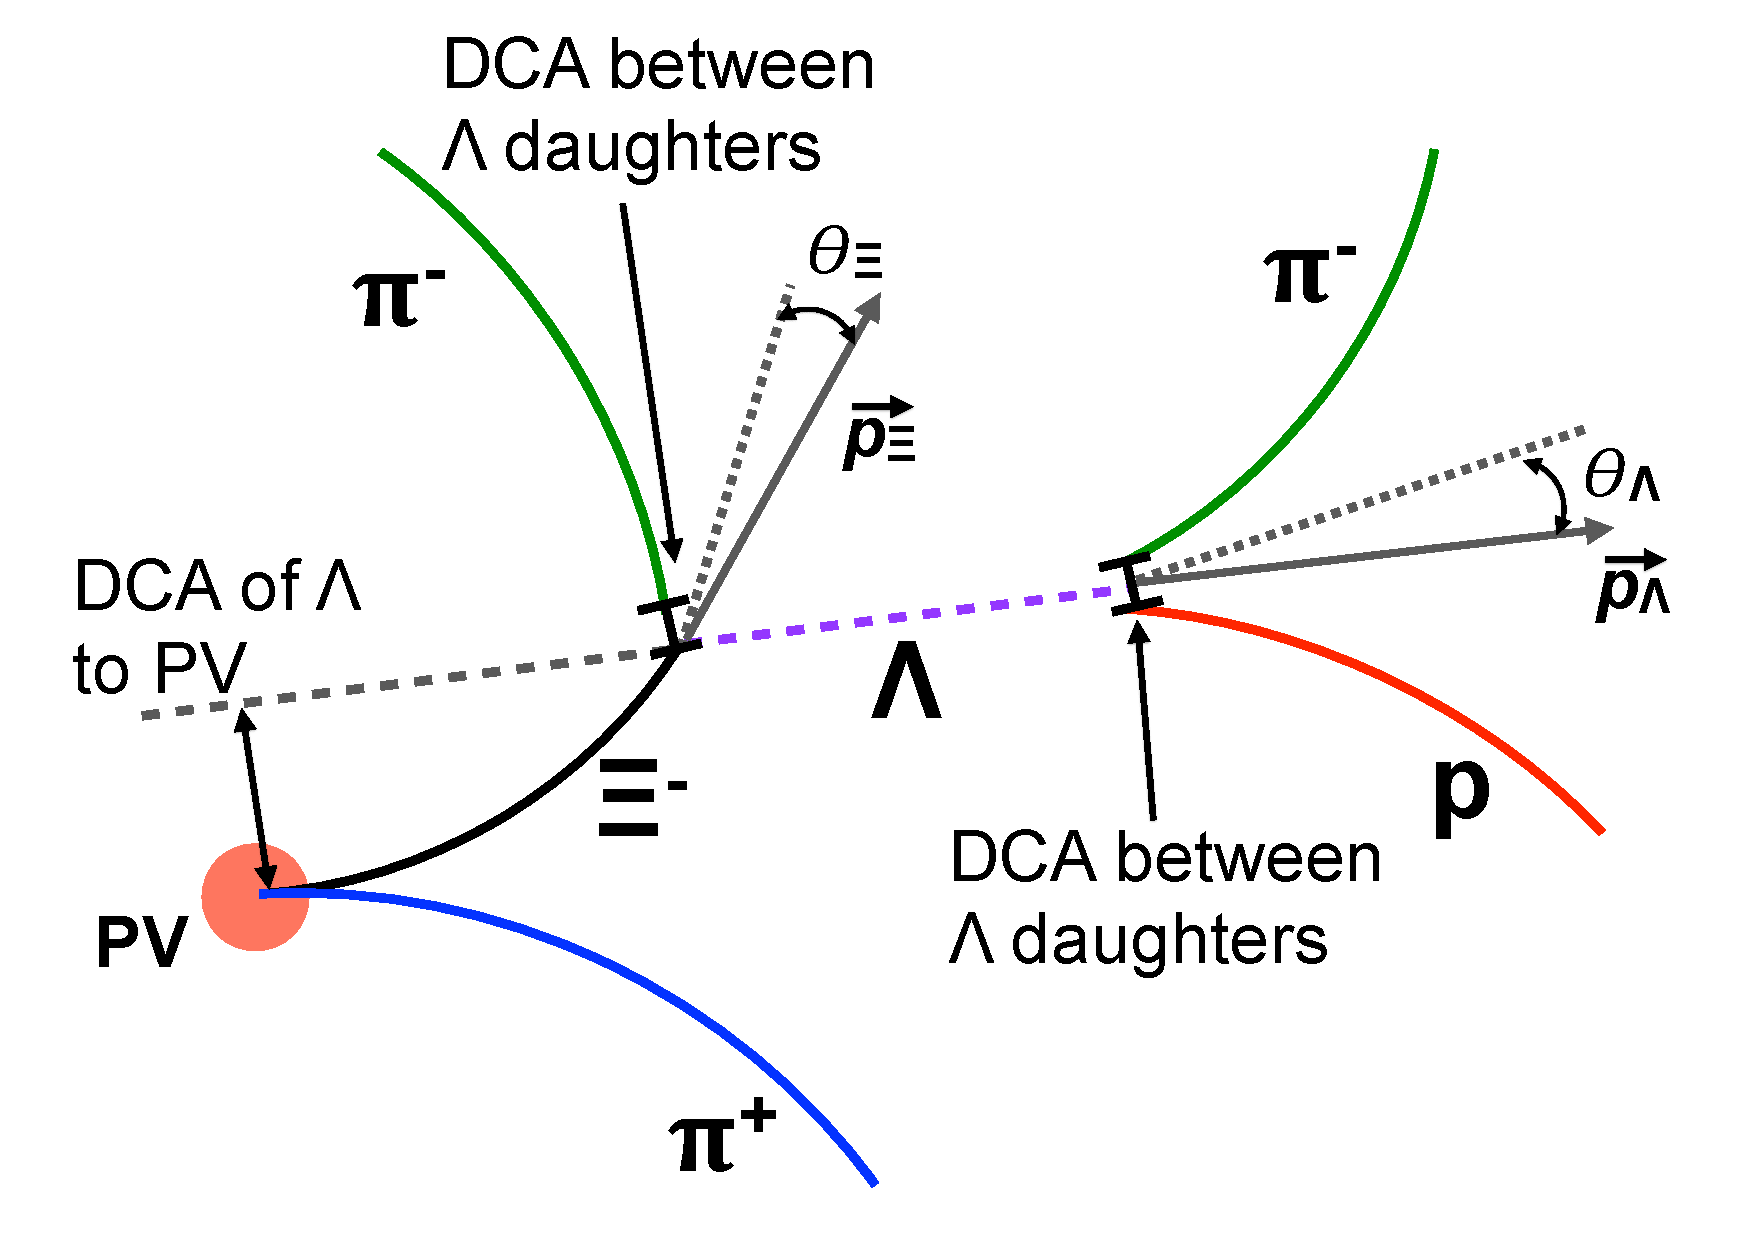
\includegraphics[width=11.cm]{./Version1/FigChapter5/Selection/Sketch.pdf}
\caption{ Sketch of the decay modes for $\Xi^{*0}$ and depiction of the track and topological selection criteria.}
\label{fig:decay}
\end{center}
\end{figure}

Since pions and protons from weak decay of $\Lambda$ ($ \cL \tau = 7.89$ cm~\cite{cite:PDG}) and 
pions from weak decay of $\Xi^{-}$ ($ \cL \tau = 4.91$ cm~\cite{cite:PDG}) are produced away from the PV, 
specific topological and track selection criteria, as summarized in Table~\ref{tab:selections}, were 
applied~\cite{ cite:Xi_pPb,cite:Xi_pp,cite:lambda_pp}.



\begin{table}[h!]
\centering
\begin{tabular}{lll}
\hline\noalign{\smallskip}
Topological cuts & p--Pb & Pb--Pb\\
\hline
DCA$_r$ of $\Lambda$ decay products to PV   & $>0.06$ cm& $>0.11$ cm \\
DCA between $\Lambda$ decay products   & $<1.4$cm & $<0.95$ cm\\
DCA of $\Lambda$ to PV                   & $>0.015$  cm& $>0.06$ \\
cos$\theta_\Lambda$ & $>0.875$  &          $>0.998$ \\
$r(\Lambda)$          & 0.2 $<r(\Lambda)<$ 100 cm   &  0.2 $<r(\Lambda)<$ 100 cm    \\
$|M_{p\pi} - m_\Lambda|$        & $<$ 7 \mmass  &$<$ 7 \mmass\\
DCA$_r$ of pion (from $\Xi^{-}$) to PV     & $>0.015$ cm &$>0.035$ cm\\
DCA between $\Xi^{-}$ decay products  & $<1.9$ cm&$<0.275$\\
cos$\theta_\Xi$     & $>0.981$    & $>0.9992$\\
$r(\Xi^-)$            & 0.2 $<r(\Xi^-)<$ 100 cm      &  0.2 $<r(\Xi^-)<$ 100 cm  \\
$|M_{\Lambda\pi} - m_\Xi|$        &  $<$ 7 \mmass  &   $<$ 7 \mmass   \\
\hline
\end{tabular}
\caption{Topological and track selection criteria.}
\label{tab:selections}. 
\end{table}

In the analysis of $\Xi^{*0}$, $\Lambda$ and $\pi$ from $\Xi^{-}$ were 
selected with a DCA of less than 1.9~cm and with a DCA$_r$ to the PV greater than 0.015 cm. 
The $\Lambda$ daughter particles ($\pi$ and p) were required to have a DCA$_r$ to the PV greater 
than 0.06 cm, while the DCA between the two particles was required to be less than 1.4 cm. Cuts on 
the invariant mass, the cosine of the pointing angle ($\theta_\Lambda$, $\theta_\Xi$) and the radius of 
the fiducial volume ($r(\Lambda)$, $r(\Xi)$) in Table~\ref{tab:selections} were applied to optimize 
the balance of purity and efficiency of each particle sample. 


\newpage
\subsubsection{Particle identification}\label{sec:pPb:PID}
PID selection criteria are applied for
 
 \begin{enumerate}
\item $\pi^{\pm}$ (last emitted $\pi$) and proton from $\Lambda$
\item $\pi^{\pm}$ (second emitted $\pi$)   from $\Xi^{\pm}$
\item $\pi^{\pm}$ (first emitted $\pi$) from  $\Xi$(1530)$^{0}$
\end{enumerate}
 by using TPC. On TPC dE/dx versus momentum distribution, 3$\sigma$ cuts are applied to TPC for selecting each of the particles. The TPC $\mathrm{d}E/\mathrm{d}x$ selection allows to have better signal with $\sim$20\% increase of significance. 
  
 
\begin{figure}[htbp]
\begin{center}
\includegraphics[width=7.0cm]{./Version1/FigChapter5/Selection/pPbTPC3rdPion.eps}
\hspace{0.5cm}
\includegraphics[width=7.0cm]{./Version1/FigChapter5/Selection/pPbTPC3rdPionAfter.eps}
\label{fig:pPb:TPCpionFirstEmitted} 
\caption{ TPC $\mathrm{d}E/\mathrm{d}x$ as function of transverse momentum for total (top) and selected first emitted $\pi$ in 3$\sigma$ (bottom) }
\end{center}
\end{figure}

 
 \begin{figure}[htbp]
\begin{center}
\includegraphics[width=7.0cm]{./Version1/FigChapter5/Selection/pPbTPC2ndPion.eps}
\hspace{0.5cm}
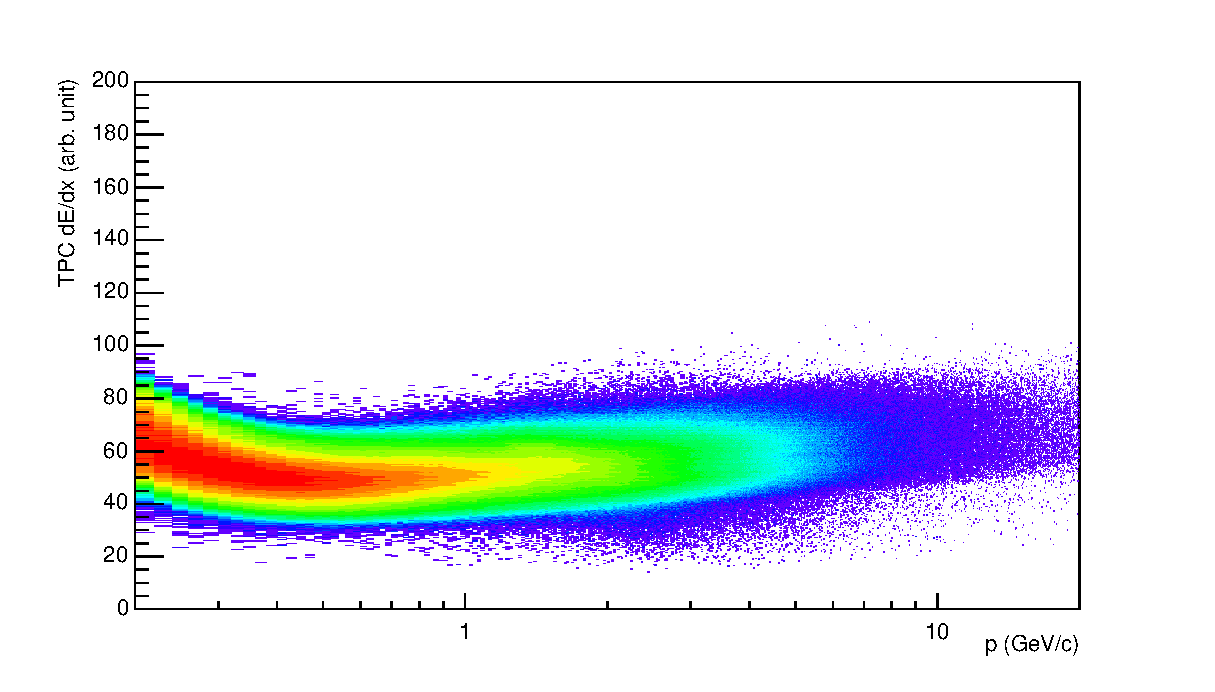
\includegraphics[width=7.0cm]{./Version1/FigChapter5/Selection/pPbTPC2ndPionAfter.eps}
\label{fig:pPb:TPCpionSecondEmitted} 
\caption{ TPC $\mathrm{d}E/\mathrm{d}x$ as function of transverse momentum for total (top) and selected second emitted $\pi$ in 3$\sigma$(bottom) }
\end{center}
\end{figure}


\begin{figure}[htbp]
\begin{center}
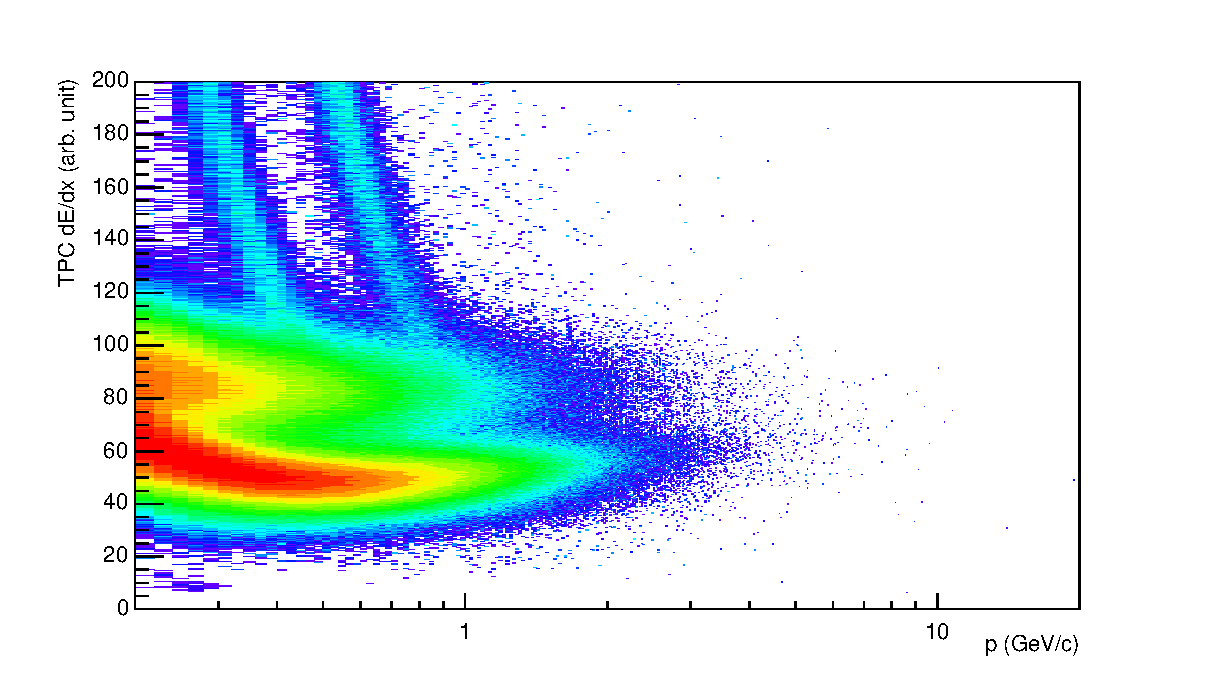
\includegraphics[width=7.0cm]{./Version1/FigChapter5/Selection/pPbTPC1stPion.eps}
\hspace{0.5cm}
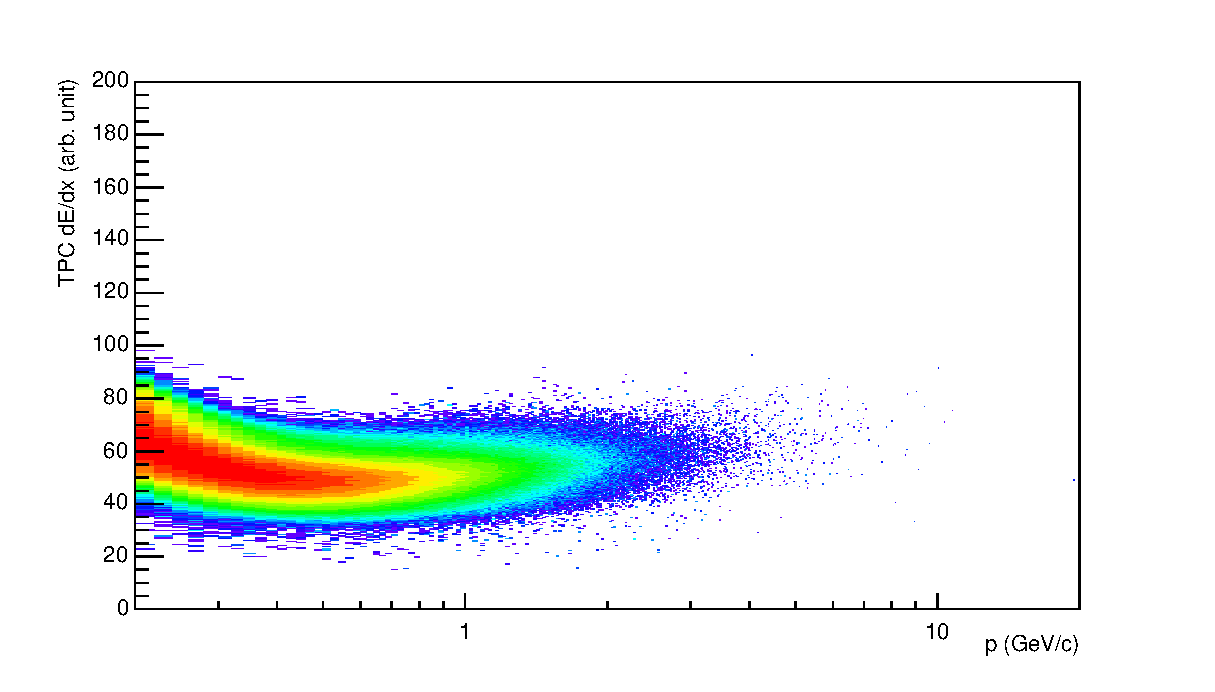
\includegraphics[width=7.0cm]{./Version1/FigChapter5/Selection/pPbTPC1stPionAfter.eps}
\label{fig:pPb:TPCpionLastEmitted} 
\caption{ TPC $\mathrm{d}E/\mathrm{d}x$ as function of transverse momentum for total (top) and selected last emitted $\pi$ in 3$\sigma$(bottom) }
\end{center}
\end{figure}


\begin{figure}[htbp]
\begin{center}
\includegraphics[width=7.0cm]{./Version1/FigChapter5/Selection/pPbTPCp.eps}
\hspace{0.5cm}
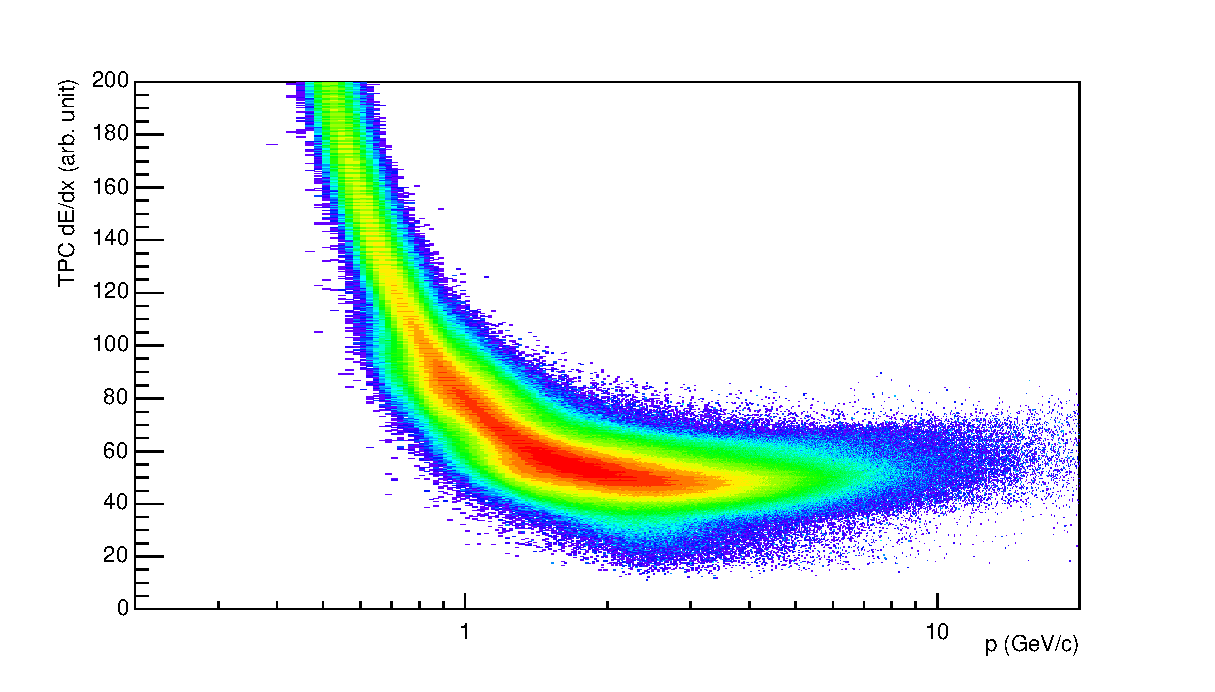
\includegraphics[width=7.0cm]{./Version1/FigChapter5/Selection/pPbTPCpAfter.eps}
\label{fig:pPb:TPCp} 
\caption{ TPC $\mathrm{d}E/\mathrm{d}x$ as function of transverse momentum for total (top) and selected proton in 3$\sigma$(bottom) }
\end{center}
\end{figure}

%%%
\begin{figure}[htbp]
\begin{center}
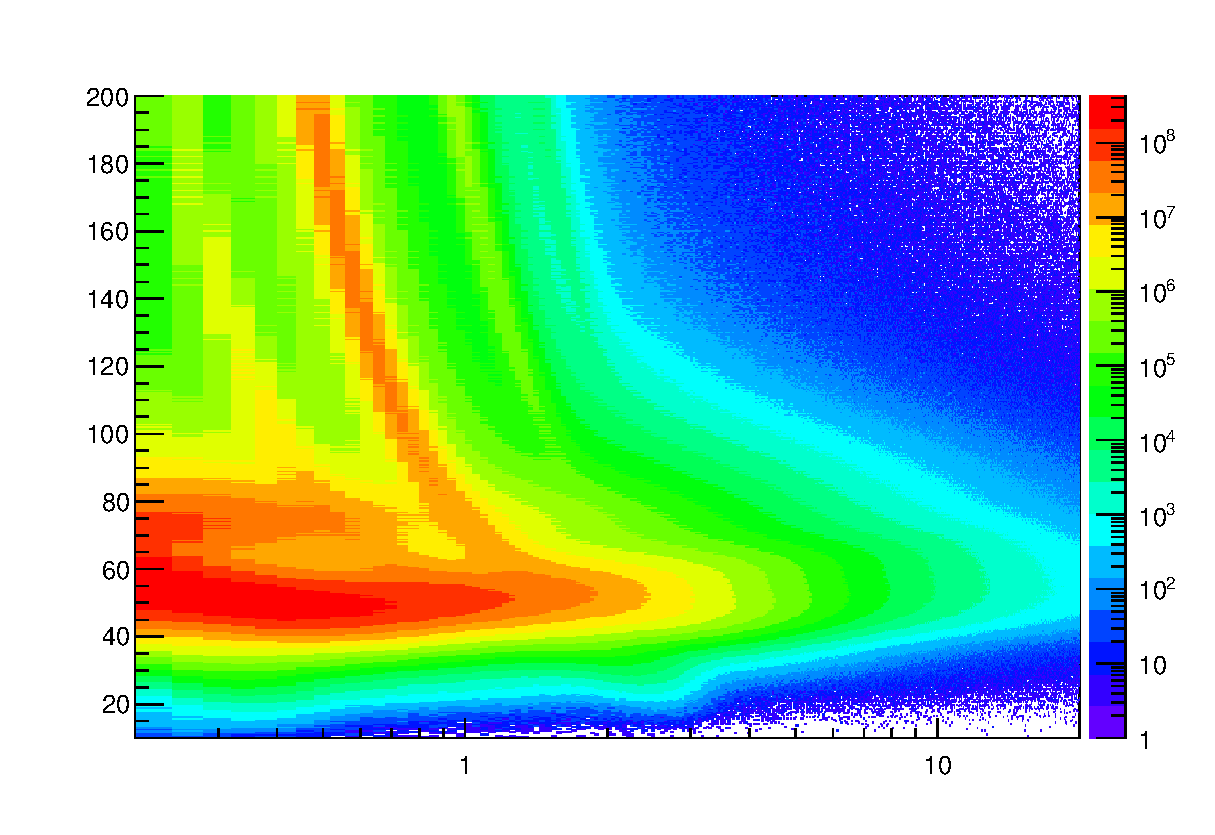
\includegraphics[width=7.0cm]{./Version1/FigChapter5/Selection/PbPbTPC3rdPion.eps}
\hspace{0.5cm}
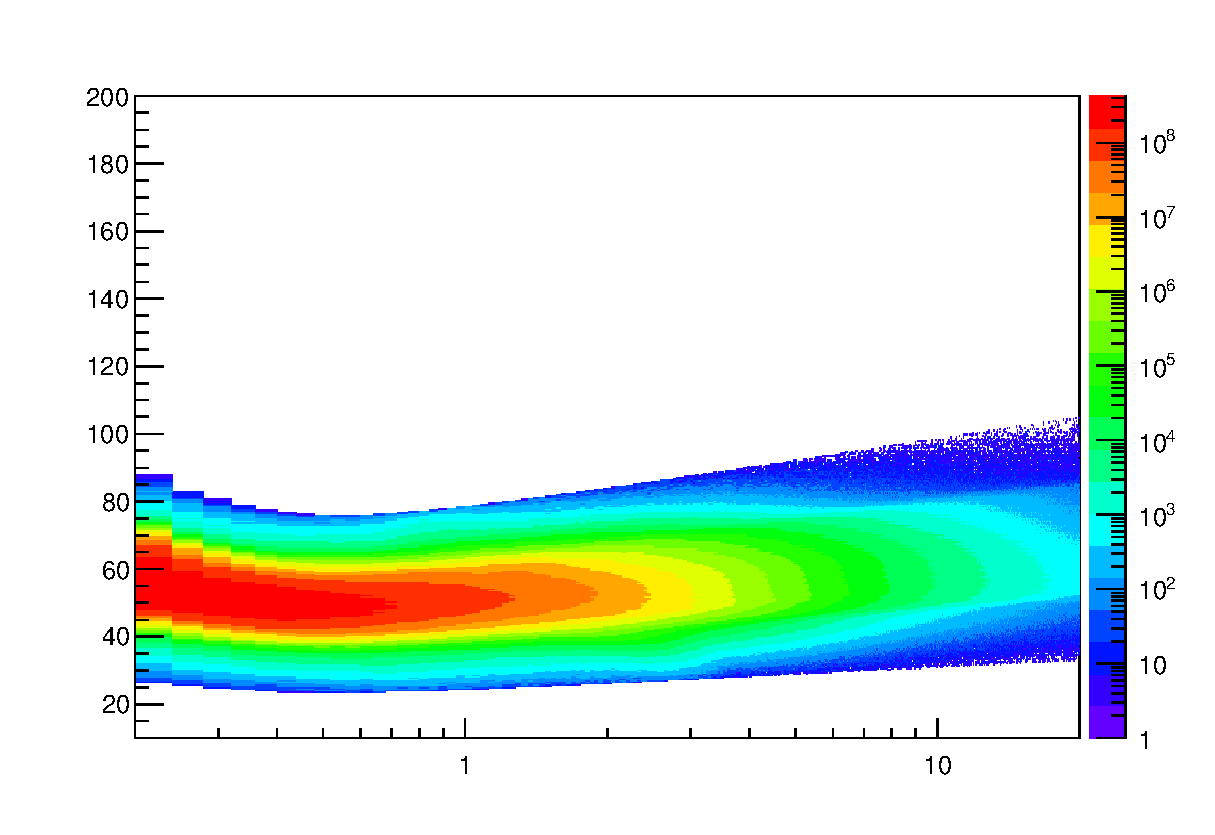
\includegraphics[width=7.0cm]{./Version1/FigChapter5/Selection/PbPbTPC3rdPionAfter.eps}
\label{fig:PbPb:TPCpionFirstEmitted} 
\caption{ TPC $\mathrm{d}E/\mathrm{d}x$ as function of transverse momentum for total (top) and selected first emitted $\pi$ in 3$\sigma$ (bottom) }
\end{center}
\end{figure}

 
 \begin{figure}[htbp]
\begin{center}
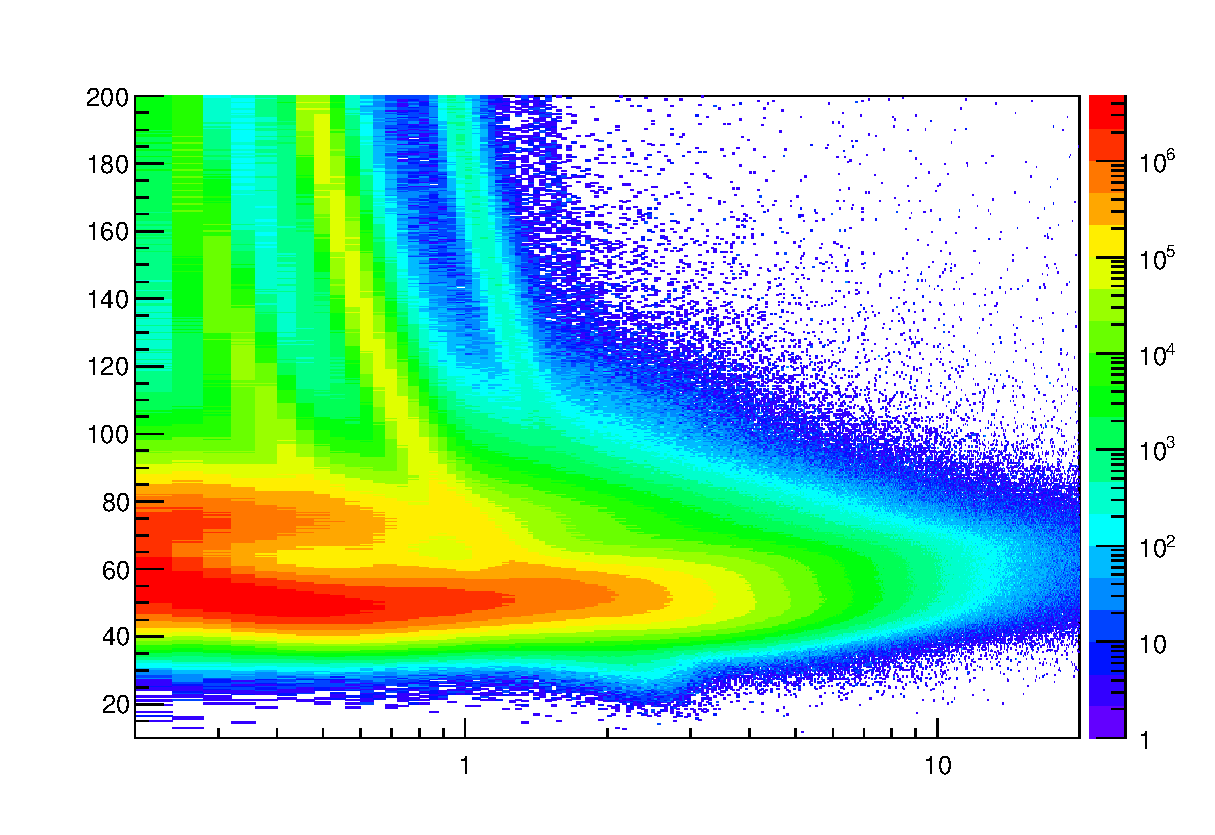
\includegraphics[width=7.0cm]{./Version1/FigChapter5/Selection/PbPbTPC2ndPion.eps}
\hspace{0.5cm}
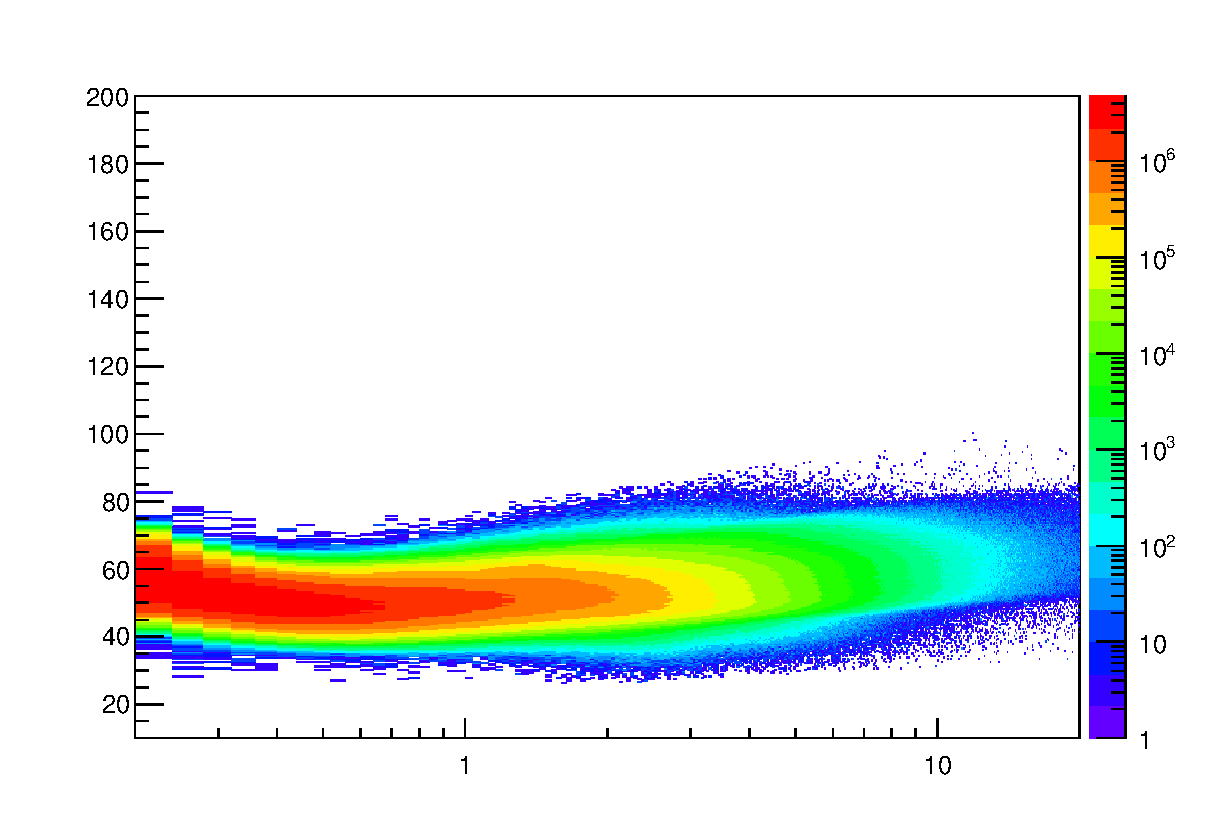
\includegraphics[width=7.0cm]{./Version1/FigChapter5/Selection/PbPbTPC2ndPionAfter.eps}
\label{fig:PbPb:TPCpionSecondEmitted} 
\caption{ TPC $\mathrm{d}E/\mathrm{d}x$ as function of transverse momentum for total (top) and selected second emitted $\pi$ in 3$\sigma$(bottom) }
\end{center}
\end{figure}


\begin{figure}[htbp]
\begin{center}
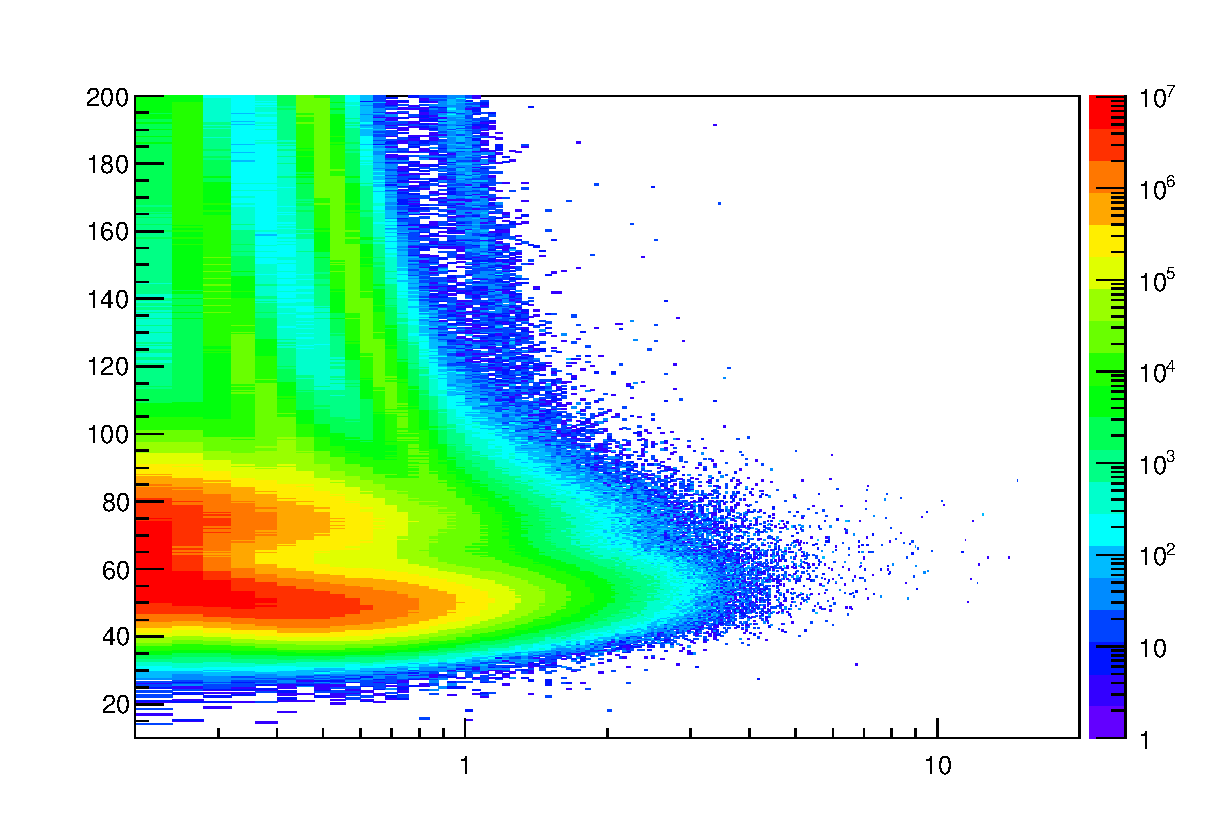
\includegraphics[width=7.0cm]{./Version1/FigChapter5/Selection/PbPbTPC1stPion.eps}
\hspace{0.5cm}
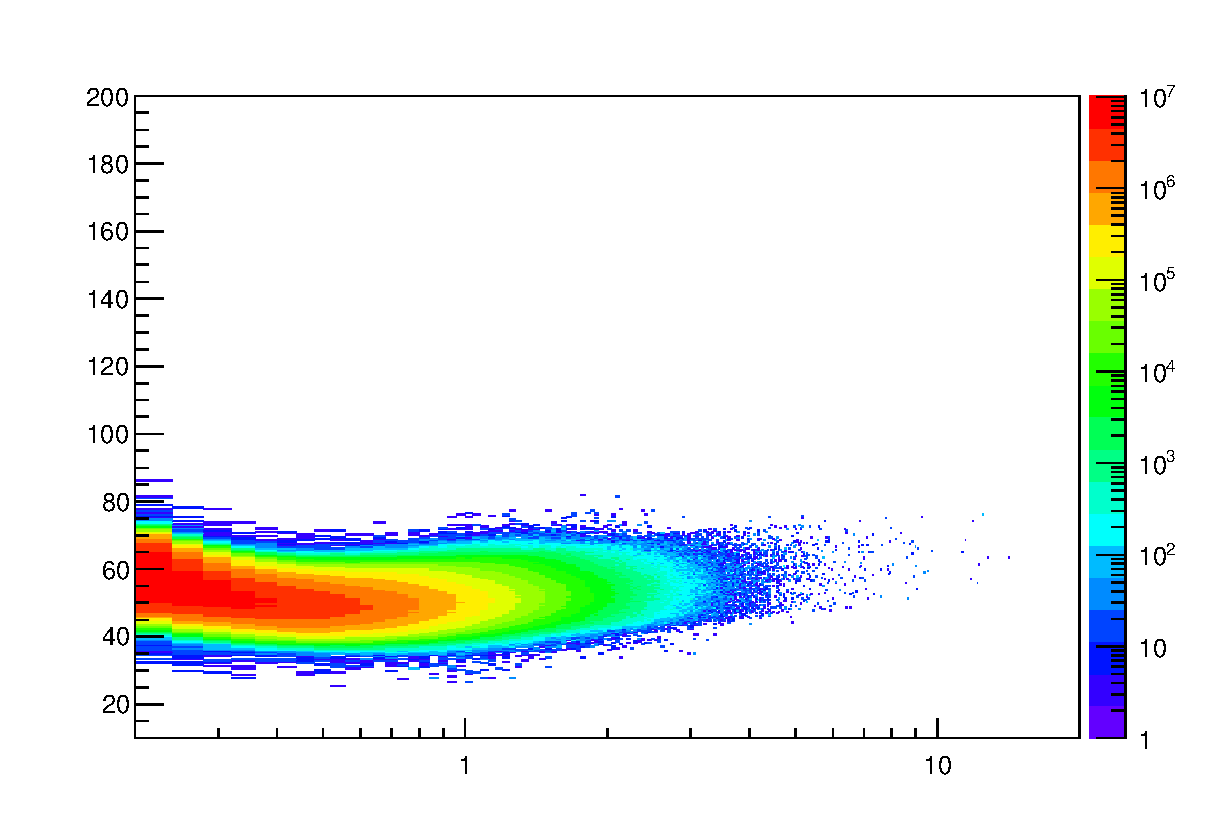
\includegraphics[width=7.0cm]{./Version1/FigChapter5/Selection/PbPbTPC1stPionAfter.eps}
\label{fig:PbPb:TPCpionLastEmitted} 
\caption{ TPC $\mathrm{d}E/\mathrm{d}x$ as function of transverse momentum for total (top) and selected last emitted $\pi$ in 3$\sigma$(bottom) }
\end{center}
\end{figure}


\begin{figure}[htbp]
\begin{center}
\includegraphics[width=7.0cm]{./Version1/FigChapter5/Selection/PbPbTPCp.eps}
\hspace{0.5cm}
\includegraphics[width=7.0cm]{./Version1/FigChapter5/Selection/PbPbTPCpAfter.eps}
\label{fig:PbPb:TPCp} 
\caption{ TPC $\mathrm{d}E/\mathrm{d}x$ as function of transverse momentum for total (top) and selected proton in 3$\sigma$(bottom) }
\end{center}
\end{figure}



 
\newpage
\subsubsection{Signal extraction}\label{sec:pPb:signal}

The $\Xi^{*0}$ signals were reconstructed by invariant-mass analysis 
of candidates for the decay products in each transverse momentum interval of the resonance 
particle, and for each multiplicity class. The  $\Xi^-\pi^+$($\Xi^+\pi^-$) invariant mass distribution is reported in Figure \ref{fig:sigpPbb} for semi-central events (20-40\%) in p--Pb collisions and Figure \ref{fig:sigPbPbb} for central events(0-10\%) in Pb--Pb collisions.


\begin{figure}[htbp]
\begin{center}
\includegraphics[width=12.0cm]{./Version1/FigChapter5/Extraction/SigpPb_Before.eps}
\hspace{0.5cm}
\label{fig:sigpPbb} 
\caption{ The $\Xi^{\mp}\pi^{\pm}$ invariant mass distribution (Same-event pairs) in 
1.8$<$ \pt $<$2.2~\gmom~and for the multiplicity class 20-40\%. The background shape, 
using pairs from different events (Mixed-event background), is normalised to the counts in 
1.49~$<$~$M_{\Xi\pi}$~$<$~1.51~\Gmass~and 1.56~$<$~$M_{\Xi\pi}$~$<$~1.58~\Gmass. }
\end{center}
\end{figure}

\begin{figure}[htbp]
\begin{center}
\includegraphics[width=12.0cm]{./Version1/FigChapter5/Extraction/SigPbPb_Before.eps}
\hspace{0.5cm}
\label{fig:sigPbPbb} 
\caption{ The $\Xi^{\mp}\pi^{\pm}$ invariant mass distribution (Same-event pairs) in 
3.0$<$ \pt $<$3.5~\gmom~and for the centrality class 0-10\%. The background shape, 
using pairs from different events (Mixed-event background), is normalised to the counts in 
1.49~$<$~$M_{\Xi\pi}$~$<$~1.51~\Gmass~and 1.56~$<$~$M_{\Xi\pi}$~$<$~1.58~\Gmass. }
\end{center}
\end{figure}

Since the resonance decay products originate from a position which is indistinguishable from the PV,
a significant combinatorial background is present. In order to extract \xis signal it is necessary to remove or, at least reduce, the combinatorial background. For this analysis, this has been done with the event mixing (EM) technique, by combining uncorrelated decay products  20 different events in p--Pb (5 different events in Pb--Pb). The events for the mixing have been selected by applying the similarity criteria to minimise distortions due to different acceptances and to ensure a similar event structure, only tracks from events with similar vertex positions $z$ ($|\Delta z| <$ 1 cm) and track multiplicities $n$ ($|\Delta n|<$ 10) were taken.

The mixed-event background distributions were normalised to two fixed regions, 
\linebreak 1.49~$<$~$M_{\Xi\pi}$~$<$~1.51~\Gmass~and 1.56$<$~$M_{\Xi\pi}$~$<$~1.58~\Gmass,
~around the $\Xi^{*0}$ mass peak (Figure \ref{fig:sigpPbb} and \ref{fig:sigPbPbb}). These regions were used for all \pt intervals and multiplicity classes, because the background shape is reasonably well reproduced in these regions and the invariant-mass resolution of the reconstructed peaks appears stable, independently of \pt. The uncertainty on the normalisation was estimated by varying the normalisation regions and is included in the quoted systematic uncertainty for the signal extraction (Section\ref{sec:sys}).

After the background subtraction, the resulting distribution is shown in Figure \ref{fig:sigpPba} and \ref{fig:sigPbPbb}. In order to obtain raw yields, a combined fit of a first-order polynomial for the residual background and a Voigtian function (a convolution of a Breit-Wigner and a Gaussian function accounting for the detector resolution) for the signal was used. The mathematical form of fit function used in anaysis is: 

\begin{equation}
f(M_{\Xi\pi})= \frac{Y}{2\pi}  \frac{\Gamma_{0}}{(M_{\Xi\pi}-M_{0})^2+\frac{\Gamma_{0}^{2}}{4}} \frac{e^{-(M_{\Xi\pi}-M_{0})/2\sigma^{2}}}{\sigma\sqrt{2\pi}} + bg(M_{\Xi\pi})
\end{equation}


\begin{figure}[htbp]
\begin{center}
\includegraphics[width=12.0cm]{./Version1/FigChapter5/Extraction/SigpPb_After.eps}
\hspace{0.5cm}
\label{fig:sigpPba} 
\caption{ The invariant mass distribution after subtraction of the mixed-event background in p--Pb collisions. 
The solid curve represents the combined fit, while the dashed line describes the residual background.}
\end{center}
\end{figure}


\begin{figure}[htbp]
\begin{center}
\includegraphics[width=12.0cm]{./Version1/FigChapter5/Extraction/SigPbPb_After.eps}
\hspace{0.5cm}
\label{fig:sigpPba} 
\caption{ The invariant mass distribution after subtraction of the mixed-event background in Pb--Pb collisions. 
The solid curve represents the combined fit, while the dashed line describes the residual background.}
\end{center}
\end{figure}

The mass parameter of the Voigtian fit ($M_{0}$) is left free within the fit range (1.48 \Gmass and 1.59 \Gmass). The overall invariant mass width of the Voigtian function is governed by 2 parameters: $\sigma$ and $\Gamma_{0}$. The $\sigma$ describes the broadening of the peak due to finite detector resolution while $\Gamma$ describes the intrinsic width of the resonance itself. The $\Gamma_{0}$ is fixed to the PDG value of 9.1 \mmom for the\xis. Because of lack of statistics, the $\sigma$ can be over estimated. Therefore the $\sigma$ parameter is fixed to value derived from $\sigma$ in MB events which has largest statistics. The $\sigma$ as function of \pt distribution in MB events is shown in Figure. \ref{fig:sigma} and we also report invariant mass of \xis as function of \pt in Figure. \ref{fig:mass}. The \xis raw yields have been extracted from the fit for the 4 multiplicity bins (+ NSD events) in p--Pb and 4 centrality bins in Pb--Pb collisions and the yields as function of \pt are shown in Figure \ref{fig:rawyield}.



\begin{figure}[htbp]
\begin{center}
\includegraphics[width=10.0cm]{./Version1/FigChapter5/Extraction/pPbWidthMB.eps}
\hspace{0.5cm}
\includegraphics[width=10.0cm]{./Version1/FigChapter5/Extraction/PbPbWidthMB.eps}
\caption{$\sigma$ fit parameters as a function of \pt in MB in p--Pb collisions (top) and in Pb--Pb collisions (bottom).} 
 \label{fig:sigma}
\end{center}
\end{figure}



\begin{figure}[htbp]
\begin{center}
\includegraphics[width=10.0cm]{./Version1/FigChapter5/Extraction/pPbMass.eps}
\hspace{0.5cm}
\includegraphics[width=10.0cm]{./Version1/FigChapter5/Extraction/PbPbMass.eps}
\caption{\xis-mass obtained from fit of the Voigtian peak as a function of \pt in each multiplicity classes in p--Pb collisions (top) and the different centrality classes in Pb--Pb (bottom).} 
 \label{fig:mass}
\end{center}
\end{figure}


\begin{figure}[htbp]
\begin{center}
\includegraphics[width=10.0cm]{./Version1/FigChapter5/Extraction/pPbRawYield.eps}
\hspace{0.5cm}
\includegraphics[width=10.0cm]{./Version1/FigChapter5/Extraction/PbPbRawYield.eps}
\caption{\xis-raw spectra obtained from fit of the Voigtian peak and a polynomial residual background for different multiplicities in p--Pb collisions (top) and Pb--Pb collisions (bottom). Only the statistical error is reported.} 
 \label{fig:rawyield}
\end{center}
\end{figure}





\newpage
\subsection{Efficiency correction}\label{sec:MC} 
The raw yields were corrected for the geometrical acceptance and the reconstruction efficiency
(A $\times$ $\epsilon$) of the detector (Figure.~\ref{fig:pPb:efficiency}). By using the DPMJET 3.05 event generator~\cite{cite:DPMJET} and the GEANT~3.21 package~\cite{cite:GEANT}, a sample of about 100 million p--Pb events was simulated and reconstructed in order to compute the corrections. The distributions of $A\times\epsilon$ were obtained from the ratio between the number of reconstructed $\Xi^{*0}$ and the number of generated particle in the same \pt~and rapidity interval. Since the correction factors for different multiplicity classes are in agreement with those from MB events within statistical uncertainty, the latter were used for all multiplicity classes.

\begin{figure}[htbp]
\begin{center}
\includegraphics[width=10.0cm]{./Version1/FigChapter5/MC/Efficiency.eps}
\caption{\xis-raw spectra obtained from fit of the Voigtian peak and a polynomial residual background for different multiplicities. Only the statistical error is reported.} 
 \label{fig:pPb:efficiency}
\end{center}
\end{figure}


Because the generated $\Xi(1530)^{0}$ spectra have different shapes than the measured \xis spectra, it is necessary to weight the generated and reconstructed \xis spectra in these simulations. Fig. \ref{fig:pPb:datagenrec} shows the generated and reconstructed \xis spectra plotted with the (corrected) measured \xis spectrum for MB events and the Levy fit of that measured spectrum. The generated and measured \xis spectra have  different behaviours for the range 0.5 $<$ $p_{\mathrm{T}}$ $<$ 1 GeV/$c$. The generated \xis spectrum decreases with increasing \pt over this range, while the fit of the measured \xis spectrum reaches a local maximum in this range. The correction $\epsilon$ is observed to change rapidly over this \pt range. It is therefore necessary to weight the generated spectrum so that it has the shape of the measured  \xis  spectrum (and to apply corresponding weights to the reconstructed \xis spectrum). An iterative procedure is performed to determine the correct weighting (and therefore the correct $\epsilon$). 
\begin{figure}[htbp]
\begin{center}
\includegraphics[width=10.0cm]{./Version1/FigChapter5/MC/Weighting.eps}
\caption{Real corrected \xis spectrum (black) for the minimum bias with Levy fit (black curve). Also shown are the unweighted generated (blue) and reconstructed (red) \xis spectra.}
\label{fig:pPb:datagenrec}
\end{center}
\end{figure}

\begin{enumerate}
\item The unweighted $\epsilon$ is calculated.
\item This $\epsilon$ is used to correct the measured xis spectrum.
\item The corrected \xis spectrum is fit.
\item This fit is used to weight the simulated xis spectra. A \pt dependent weight is applied to the generated xis spectrum so that it follows the fit. The same weight is applied to the reconstructedxis spectrum.
\item The (weighted) $\epsilon$ is calculated.
\item Steps 2-5 are repeated (with the weighted $\epsilon$ from step 5 used as the input for step 2) until the $\epsilon$ values are observed to change by $<$ 0.1\% (relative) between iterations. It is observed that four iterations are sufficient for this procedure to converge.
\end{enumerate}

Finally, the re-weighted efficiency is obtained and the distribution as function of \pt is shown in Figure \ref{fig:pPp:mbefficiency}.

\begin{figure}[htbp]
\begin{center}
\includegraphics[width=10.0cm]{./Version1/FigChapter5/MC/MBEfficiency.eps}
\caption{Efficiency as a function of \pt in minimum bias events in p--Pb collisions.} 
 \label{fig:pPp:mbefficiency}
\end{center}
\end{figure}


In order to obtain the correction factor dedicated in Pb--Pb collisions, MC events are generated using Heavy Ion Jet Interaction Generator (HIJING). The generated events are passed through a GEANT3 model of the ALICE experiment with a realistic description of the detector response. Because we have observed centrality dependent efficiency, the centrality dependent efficiencies have been applied to get corrected raw yield. The reweighing approach which was used to correct the efficiency in p--Pb is also applied to the efficiency obtained in Pb-Pb. 

\begin{figure}[htbp]
\begin{center}
\includegraphics[width=10.0cm]{./Version1/FigChapter5/MC/PbPbEfficiency.eps}
\caption{Efficiency as a function of \pt in different centrality classes in Pb--Pb collisions} 
 \label{fig:PbPb:efficiency}
\end{center}
\end{figure}


\newpage
\subsection{Corrected \pt-spectra}\label{sec:pPb:spectra} 

The $p_{\mathrm{T}}$ spectrum is by the number of produced particles of a given type in the desired interval of phase-space divided by the number of inelastic collisions. The spectrum is calculated as:

\begin{equation}
\frac{1}{N} \times \frac{d^{2}N}{dydp_{T}} = \frac{1}{N_{E,PhysSel}} \times \frac{N_{raw}}{dp_{T}dy}  \frac{1}{\epsilon} \frac{N_{total}^{MC}}{N_{post-PV cut}^{MC}}   ,
\end{equation}

where N$_{E}$ represent the number inelastic collisions, the $\frac{dN}{dydp_{T}}$ is the yield  per range of rapidity $y$, per range in \pt. On the right hand side N$_{E,PhysSel}$ is the number of events counted by the physics selection trigger. N$_{raw}$ is the raw extracted number of particle in the rapidity and \pt bin of width $\Delta y$ = 0.5 in p--Pb ($\Delta y$ = 1.0 in Pb--Pb) and $\Delta$p$_{T}$, respectively. $\epsilon$ is the reconstruction efficiency estimated from Monte Carlo simulations. $\frac{N_{total}^{MC}}{N_{post-PV cut}^{MC}}$ is the ratio of the total number of particle from MC divided by the number of particle from MC after the Primary-Vertex cut is imposed. It takes into account the fraction of particle lost after imposing the PV cut. We notice that for minimum-bias results in p--Pb, we adopted a normalisation such that to provide result from non-single diffractive(NSD) cross-section. The normalisation factor is 0.964 \cite{cite:KphipPb}. The obtained spectrum at MB and the spectrums from different multiplicity classes in p--Pb are shown in Figure \ref{fig:pPb:rawspectra} and different centrality classes in Pb--Pb are shown in Figure \ref{fig:PbPb:rawspectra}.

\begin{figure}[htbp]
\begin{center}
\includegraphics[width=10.0cm]{./Version1/FigChapter5/Spectra/StatSpectrapPb.eps}
\caption{Corrected \pt-spectra of \xis in NSD and different multiplicity classes in p--Pb collisions.} 
 \label{fig:pPb:rawspectra}
\end{center}
\end{figure}

\begin{figure}[htbp]
\begin{center}
\includegraphics[width=10.0cm]{./Version1/FigChapter5/Spectra/StatSpectraPbPb.eps}
\caption{Corrected \pt-spectra of \xis in different centrality classes in Pb-Pb collisions.} 
 \label{fig:PbPb:rawspectra}
\end{center}
\end{figure}



\newpage
\subsection{Systematic uncertainties}\label{sec:sys} 


The systematic uncertainties are calculated in seven principle groups. The procedure to obtain the systematic uncertainties is performed many times by varying the possible permutation of the analysis parameter.The general strategy for evaluating systematic uncertainties is described as following:

\begin{enumerate}
\item Choose one set of parameters for the analysis as default
\item Observe the deviation of yield when one parameter is changed
\item The systematic uncertainty is calculated for a given source as the RMS deviation of the available sources.
\item The total systematic uncertainty, taking into account all the different sources, is the sum in quadrature of each source.
\end{enumerate}

To study the systematic effect we repeat the measurement by varying one parameter at a time. 
A Barlow \cite{cite:Barlow} check has been performed for each measurement to verify whether it is due to a systematic effect or a statistical fluctuation. Let each measurement be indicated by ($\it{y}_{i}$$\pm$$\sigma_{i}$) and the central value (default measurement) by ($\it{y}_{c}$$\pm$$\sigma_{c}$), one can define $\Delta\sigma_{i}$ (Eq. \ref{eq:barlow}).


\begin{equation}
 \Delta\sigma_{i} = \sqrt(|\sigma_{i}^{2} - \sigma_{c}^{2}|)
 \label {eq:barlow}
\end{equation}

Then we calculate $\it{n}_{i}$ = $\Delta\it{y}_{i}$/ $\Delta\sigma_{i}$, where  $\Delta\it{y}_{i}$ = $|$$\it{y}_{c}$ - $\it{y}_{i}$$|$.
If $\it{n}_{i}$ $\leq$ 1.0 then the effects are due to the statistical fluctuation and if $\it{n}_{i}$ $>$ 1.0 we apply consistency check. Since the alternate and default measurements are not statistically independent, an alternate measurement which is statistically consistent with the default measurement should not be used in calculating a systematic uncertainty. The difference between the two measurements is $\Delta$ = $\it{y}$$_{c}$ - $\it{y}$$_{i}$. The difference in quadrature of the uncertainties is calculated by Eq. \ref{eq:barlow}. 
It could be possible to check if $\Delta$$<$ $\sigma$ and exclude such cases from the systematic uncertainties. However, there can be statistical fluctuations for which $\Delta$$>$ $\sigma$. If the variations between the default and alternate measurements are purely statistical, the distribution of $\Delta$$/$$\sigma$ should be a Gaussian with a mean value that is consistent with zero and a deviation $\sigma$ consistent with unity. In this analysis, if the mean value is less than 0.1 and $\sigma$ is less than 1, the variation passes the consistency check.

Only the measurements which passed the Barlow check ($\it{n}_{i}$ $>$ 1) are used to determine the systematic uncertainty. For measurements N $>$ 2, the systematic uncertainty has been determined as the RMS (eqn. \ref{eq:rms}) of the available measurements. If N=2, the absolute difference is assigned as systematic uncertainty.

\begin{equation}
\delta y_{syst.}=\sqrt{\frac{1}{N}\sum_{i}(y_{i}-\overline{y})^{2}}
\label{eq:rms}
\end{equation}

Here N is the total number of available measurements including $\it{y}_{c}$ and $\overline{\it{y}}$ is the average of value of the measurements. The measurement did not pass Barlow check, zero systematic uncertainty has been assigned to the value.

By suing the way as explained above, all the main contributions to the systematic uncertainty of particle spectra have been studied. In particular those that comes from signal extraction, topological and kinematical selection cuts, track quality selection and n$\sigma$ TPC PID variation. the meaning of each source of systematic uncertainty studied is described in the following: \\

\textbf{Signal extraction}\\
We have extracted the signal with varying the yield calculating method which contains the method of signal extraction by integrating the Voigtian fit function and bin counting. We also have varied the normalisation range which is related to the invariant mass region where the mixed events distribution is scaled to subtract the combinatorial background and different background estimator such as Like-Sign distribution and polynomial fit was taken account into the systematic source of signal extraction. The systematic uncertainty from signal extraction is sum in quadrature of three sources. \\


\textbf{Topological selection}\\
To evaluate the stability of the chosen set of values for the topological cuts, loose and tight cuts have beed defined in order to vary by $\pm$10\% respectively. The parameters are changed once at a time. Total systematic uncertainty from topological selection is calculated by summation in quadrature of nine sources.\\


\textbf{TPC N$_{cluster}$ selection}\\
The selection performed for the daughter tracks of the cascade is that N$_{cluster}$ is larger than 70 and the value has been varied to 60 and 80 in order to estimate the systematic uncertainty  due to this selection. \\


\textbf{TPC $\mathrm{d}E/\mathrm{d}x$ selection}\\
In order to evaluate any potential effect due to the TPC $\mathrm{d}E/\mathrm{d}x$ selection (U$_{PID}$), the N$_{\sigma}$ selection was varied with N = 2.5 and 3.5. \\


\textbf{\pt~shape correction}\\
As described in Section \ref{sec:MC}, due to the different shape of the measured and generated \xis spectra, we have applied reweighing procedure to the generated spectra to have same shape and this correction is added into contributor of systematic uncertainty as \pt~shape correction.\\

\textbf{Mass window range selection}\\
In order to select $\Xi^{\pm}$ which is daughter particle of \xis, we apply the mass window $\pm$7 \mmass~around \xis mass on $\Lambda$$\pi$ invariant mass distribution. The boundaries has been varied to $\pm$6 \mmass~and $\pm$8 \mmass~to estimate systematic uncertainty.\\
 

\textbf{Vertex range selection}\\
The distribution of vertex-z is shown in Fig.\ref{fig:VzDistribution}. The cut on $|$Vz$|$ was varied from the nominal $\pm$10cm to $\pm$9cm, $\pm$11cm.\\

\textbf{Material Budget and hadronic cross section}\\
A possible source of uncertainty comes from the description of the material, active (detecting area) or dead (structure and cable), that the particles cross during their travel in the MC with respect to the real material present in the detector. Such description could affect the reconstruction efficiency in different aspects (e.g. multiple scattering, energy loss). The value estimated by $\Xi$ analysis \cite{cite:strangePbPb} has been used in this study which gives 4\% systematic uncertainty. In case of systematic uncertainty from hadronic cross section, we have inherited the value studied in previous measurement\cite{cite:trackingeffi} which amount is 1\%.\\

\textbf{Tracking efficiency}\\
Systematic uncertainties from tracking efficiency from ITS + TPC combined track were assigned as 3\% in p--Pb and  4\% in Pb--Pb collision system.\cite{cite:trackingeffi} \\
(https://twiki.cern.ch/twiki/bin/view/ALICE/TrackingEfficiencyCharged)\\


Finally, total systematic uncertainty is sum in quadrature of sources listed above. Figure \ref{fig:pPb:syserrortot} and Figure \ref{fig:pPb:syscent} show the total systematic uncertainty in minimum bias event and different multiplicity classes in p--Pb collisions, respectively. Again, Figure \ref{fig:PbPb:syserrortot} and Figure \ref{fig:PbPb:syscent} present the total systematic uncertainty in minimum bias event and different centrality classes in Pb--Pb collisions.


\begin{figure}[htbp]
\begin{center}
\includegraphics[width=12.0cm]{./Version1/FigChapter5/Systematic/pPbSysTotalFinal.eps}
\caption{Summary of the contributions to the systematic uncertainty in minimum bias events in p--Pb collisions. The dashed black line is the sum in quadrature of all the contributions.} 
\label{fig:pPb:syserrortot}
\end{center}
\end{figure}

\begin{figure}[htbp]
\begin{center}
\includegraphics[width=12.0cm]{./Version1/FigChapter5/Systematic/pPbCent.eps}
\caption{Systematic uncertainties for each multiplicity classes in p--Pb collisions.} 
\label{fig:pPb:syscent}
\end{center}
\end{figure}


\begin{figure}[htbp]
\begin{center}
\includegraphics[width=12.0cm]{./Version1/FigChapter5/Systematic/PbPbSysTotalFinal.eps}
\caption{Summary of the contributions to the systematic uncertainty in minimum bias events in Pb--Pb collisions. The dashed black line is the sum in quadrature of all the contributions.} 
\label{fig:PbPb:syserrortot}
\end{center}
\end{figure}


\begin{figure}[htbp]
\begin{center}
\includegraphics[width=12.0cm]{./Version1/FigChapter5/Systematic/PbPbCent.eps}
\caption{Systematic uncertainties for each multiplicity classes.} 
\label{fig:PbPb:syscent}
\end{center}
\end{figure}



\begin{table}[h!]
\centering
\begin{tabular}{lcc}
\hline\noalign{\smallskip}
Source of uncertainty &   p-Pb & Pb-Pb \\

\hline\noalign{\smallskip}
\pt-dependent & & \\
\hline\noalign{\smallskip}
Tracking efficiency & 3\% & 4\% \\
Tracks selection & 1-2\% &  1-5\% \\
Topological selection & 1-2\% & 5-8\% \\
PID  & 3-7\% &  4-20\% \\ 
Signal extraction & 1-5\% & 1-4\% \\
\pt~shape correction & - & 0-8\% \\
Mass window ($\Xi^\pm$)& 4\% &  - \\
Vertex selection & 3\% & - \\
\hline\noalign{\smallskip}
\pt-independent & & \\
\hline\noalign{\smallskip}
Hadronic interaction &  - &  1\% \\
Material budget  & 4\% &  4\% \\
Branching ratio  & 0.3\% & 0.3\% \\
\hline\noalign{\smallskip}
Total & 8-12\% & 9-25 \% \\
\hline\noalign{\smallskip}
\end{tabular}
\caption{Summary of the systematic uncertainties on the differential yield, \dndydpt. 
Minimum and maximum values in all \pt~intervals and multiplicity classes in p--Pb, centrality classes in Pb--Pb are shown for 
each source.}
\label{tab:sys}    
\end{table}


\newpage
\subsection{\xis~transverse momentum spectra}\label{sec:pPb:spectra} 
The raw yield shown in Figure \ref{fig:pPb:rawspectra} and \ref{fig:PbPb:rawspectra} have been corrected for efficiency as described in section \ref{sec:MC}. The measured spectra for (\xis+\xisb)/2 are reported in Figure \ref{fig:pPb:spectrasysstat} for p--Pb collisions and Figure \ref{fig:PbPb:spectrasysstat} for Pb--Pb collisions. The statistical and systematic uncertainties are reported respectively as the error bars and the boxes on the plot. The corrected yields for p--Pb collisions are measured with  0.8$<$ \pt $<$ 8.0 \gmom~while the yields for Pb--Pb collisions are obtained with 1.2 $<$ \pt $<$ 6.0 \gmom~due to difficulty of signal extraction in low and high \pt~region. 

\begin{figure}[htbp]
\begin{center}
\includegraphics[width=12.0cm]{./Version1/FigChapter5/Spectra/SpectraStatSyspPb.eps}
\caption{Corrected yields as function of \pt~in NSD events and multiplicity dependent event classes in p--Pb collision system. Statistical uncertainties are presented as bar and systematical uncertainties are plotted as boxes.} 
\label{fig:pPb:spectrasysstat}
\end{center}
\end{figure}


\begin{figure}[htbp]
\begin{center}
\includegraphics[width=12.0cm]{./Version1/FigChapter5/Spectra/SpectraStatSysPbPb.eps}
\caption{Corrected yields as function of \pt~in different centrality classes in Pb--Pb collision system. Statistical uncertainties are presented as bar and systematical uncertainties are plotted as boxes.} 
\label{fig:PbPb:spectrasysstat}
\end{center}
\end{figure}






%\section{Data analysis}
%\subsection{Particle identification}
%\subsection{Topological reconstruction}
%\subsection{$\xis$(1530) analysis in p--Pb and Pb--Pb}
%\subsubsection{Data sample and event selection}
%\subsubsection{Topological selection}
%\subsubsection{Efficiency correction}
%\subsubsection{Systematic uncertainties}

\section{Results}
%\subsection{$\pt$-spectra}
\subsection{d$N$/d$y$ and $\mpt$}
\subsection{Particle yield ratios}
\subsubsection{Comparison with other resonances}
\subsubsection{Comparison with models}
%\section{Results}
%\subsection{$\pt$-spectra}
%\subsection{d$N$/d$y$ and $\mpt$}
%\subsection{Particle yield ratios}
%\subsubsection{Comparison with other resonances}
%\subsubsection{Comparison with models}

\bibliographystyle{utphys}
\bibliography{Reference}{}
%\bibliography{Ref}{}


\newenvironment{acknowledgement}{\relax}{\relax}
\begin{acknowledgement}
\section*{Acknowledgements}
%\input{acknowledgements_march2013.tex}    %%%%%%% get the lates version before submitting
\end{acknowledgement}



\end{document}  